\documentclass{article}
\usepackage{geometry}
\usepackage{graphicx}
\usepackage{hyperref}
\usepackage{subcaption}
\usepackage[numbers,comma,square,sort&compress]{natbib}
\geometry{a4paper,scale=0.9}
\graphicspath{{sjet_cshape_draft_images/}}
\linespread{1.0}
\bibliographystyle{unsrt}

\begin{document}

\begin{center}
\LARGE Synthetic Jet cavity shape optimization\\
powered by Reinforcement Learning\\
\end{center}

\begin{center}
\renewcommand{\thefootnote}{\fnsymbol{footnote}}
Xu Dong$^{1,}$\footnote{Contributing author, Email: me@donx.im}\\
$^{1}$\textit{Department of Mechanics, Shanghai University, Shanghai 200444, China}
\end{center}

\begin{center}
Keywords: Reinforcement Learning, Synthetic Jet, optimization design, flow analysis
\end{center}

\section*{Abstract}
\addcontentsline{toc}{section}{\protect\numberline{}Abstract}\indent

Due to characteristics of periodicity and zero-net-mass-flux, flow control based on synthetic jet without requirement of external flow input has its own advantages.
However, the fierce inner flow requires a strong synthetic device design.
Aiming to lower the pressure its chamber bears while ensuring output jet performance, this research uses machine learning method with computational fluids dynamics to optimize the chamber shape of synthetic jet device.
Different from traditional experience-reliant geometry shape optimization of flow device, this research achieves optimization without dependence on experience by applying reinforcement learning method with robustness designs.
Using different reinforcement learning algorithms and control point number, we try to optimize with different physics parameters and obtain some well-performing chamber shapes.
Then we analyze the flow characteristics and the optimization mechanisms of different optimized shapes under different physics parameters based on computational fluid dynamics numerical simulations.
The distinctive shape designs from reinforcement learning and our analyses of their fluid mechanisms may help future theoretical researches and device productions.

\section*{Introduction}
\addtocounter{section}{1}
\setcounter{subsection}{0}
\addcontentsline{toc}{section}{\protect\numberline{}Introduction}\indent

\subsection{Synthetic Jet}\indent

Since the 1990s, many researchers have focused on synthetic jets and their applications in flow control, conducting extensive research from basic definitions to experiments and numerical simulations.
As shown in Figure \ref{fig:synthetic_jet_structure}, the outlet of the synthetic jet device is above the chamber, and the bottom is a periodically vibrating diaphragm, where the diaphragm vibrates according to a periodic pattern similar to a sine function.
Under different vibration excitations, chamber shapes, and chamber sizes, the velocity, frequency, and other attributes of the synthetic jet device output flow will also change.

\begin{figure}[htbp]
    \centering
    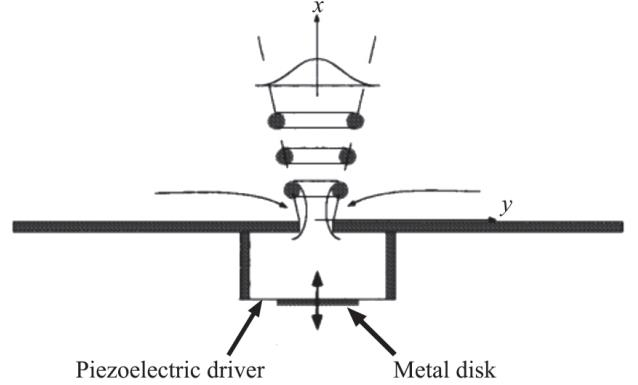
\includegraphics[width=0.32\textwidth]{synthetic_jet_structure.png}
    \captionsetup{font=scriptsize}
    \caption{
    Basic structure of a synthetic jet device.
    Its bottom vibrating membrane can be excited by methods such as piezoelectric ceramics.
    }
    \label{fig:synthetic_jet_structure}
\end{figure}

Due to the uniqueness of the synthetic jet design, it can periodically output jets at the same frequency as the bottom vibrating diaphragm without external fluid mass input.
Therefore, it is also known as a zero-net-mass-flux-jet.
When the bottom diaphragm is in the half-cycle of compressing into the chamber, the fluid inside moves upward under compression, converges at the outlet, and is ejected.
When the diaphragm is in the half-cycle of expanding outward from the chamber, external fluid enters the chamber from the top ``outlet'' due to the ``negative pressure'' effect of the diaphragm.
Thus, the synthetic jet device works without additional fluid injection, only drawing in or expelling a portion of the fluid from or to the external flow as needed.
This process is periodic and overall does not affect the mass flow rate of the external flow, but the operation of the synthetic jet clearly exerts an influence on the external flow.

By adjusting the parameters of the synthetic jet device, it is possible to produce effects desired by researchers on the external flow.
Flow control based on synthetic jets does not require additional fluid injection, making it more convenient than traditional flow control.
Relevant researchers have studied synthetic jets and explored many application scenarios. 
Shi Qing et al. used numerical simulation to study synthetic jets;
Li Chaolong et al. used numerical simulation to study the influence of synthetic jets on flow separation around a cylinder;
Peng Xuanyu et al. used numerical simulation to study the influence of synthetic jets on the lift and drag of a 2D square cylinder;
Cheng Shuiyan et al. used numerical simulation to study the regulation effect of synthetic jets on airfoil boundary layer flow;
Yang Shengke et al. combined an electric heating system with a synthetic jet actuator to study the device's protective effect against ice overflow on wings in experiments;
Li Biaohui et al. experimentally studied the impact of underwater synthetic jets on turbulent boundary layers over flat plates;
Zhu Jian et al. used numerical simulation to study the influence of synthetic jets on flow field disturbances at different excitation velocities and frequencies;
Yang Dangguo et al. experimentally studied the regulation effect of synthetic jets on aerodynamic noise in open cavities;
Han Zhonghua et al. used numerical simulation to study the role of synthetic jets in delaying airfoil stall;
Lyu Chen et al. experimentally studied the cooling characteristics of synthetic jets on computer graphics cards.

On one hand, researchers have widely applied synthetic jets in flow control;
on the other hand, to interact and couple with the flow and play an effective regulatory role, the fluid motion intensity inside the synthetic jet chamber is often high, which places high demands on the device's strength.
This paper emphasizes the impact of fluid motion within the chamber on wall pressure.
Specifically, the goal is to reduce the wall pressure integral and maximum wall pressure during the synthetic jet cycle while ensuring the device's exit velocity performance.

Traditionally, geometric shape optimization of flow devices is a difficult point.
Broadly speaking, shape optimization involves two steps.
First, it is necessary to determine which parameters may affect the optimization objective.
The number of parameters affecting the objective can be large, and judgment relies primarily on experience.
Second, determining the influence of parameters on the objective to propose targeted improvements for better performance also relies heavily on experience.

Recent developments in Artificial Intelligence have brought a new perspective to this problem: reinforcement learning can be used to achieve automatic optimization without relying on human experience.
Previously, researchers have used reinforcement learning to design airfoils and the others.

\subsection{Reinforcement Learning}\indent

\subsubsection{The three major schools of Artificial Intelligence}\indent

Since the 1950s, AI technology has developed continuously and can be roughly divided into three schools internally.

1) Symbolism: The principles of Symbolism are mainly the physical symbol system hypothesis and the principle of effective rationality.
This school believes that the basic units of human cognition and thinking are symbols, and the cognitive process is a kind of operation or calculation on symbol representations, dedicated to using computer logic symbol deduction to simulate human thinking logic.

2) Connectionism: Connectionism believes that artificial intelligence stems from imitating neurons and their neural network activities in the brain.
Its principles are mainly neural networks and the connection mechanisms and learning algorithms between them.
This school believes that human intelligence activities are the result of parallel operations of networks formed by complex connections of a large number of simple units,
emphasizing the interaction of neurons.
The main idea of Connectionism is to set up simple artificial neurons at the software or hardware level and connect them in a certain way to form complex artificial neural networks, simulating the brain's operation.
Various ``neural networks'' such as Deep Neural Networks (DNN) and Convolutional Neural Networks (CNN) are products of Connectionist thought.

3) Behaviorism: The principle of Behaviorism is cybernetics and perception-action control systems, believing that intelligence is the interaction between a system and its environment.
The idea of Behaviorism and the term itself originated from a psychological school in the early 20th century, which believed that organisms could perceive and adapt to the environment and then react, with the basic paradigm being ``perception-behavior''.
This thought was valued by researchers in other natural science fields and gradually developed into the idea of cybernetics.
By applying cybernetic ideas to AI, researchers gradually developed the Behaviorist school of AI.

The reinforcement learning algorithm used in this paper is a product of Behaviorist thought.
AlphaGo, which defeated top Go players a few years ago, deeply applied reinforcement learning algorithms and achieved remarkable results.

\subsubsection{Basic theory of Behaviorism and Reinforcement Learning}\indent

Considering the close link between Behaviorism in AI and Behaviorism in psychology, and to further introduce the basic methods of the Behaviorist school, some content from the field of Behaviorist psychology is supplemented here.
Behaviorist psychologists believe that behavior is a combination of physical responses made by organisms to adapt to environmental changes, believing that specific behavioral responses depend on specific stimulus intensities, summarized as the ``stimulus-response'' model.
Behaviorist psychologists further believe that the task of psychology is to discover the regular connection between stimulus and response, so that response can be inferred from stimulus, or stimulus can be inferred from response, thereby achieving prediction and control of behavior.

More specifically, the basic idea of reinforcement learning mainly stems from psychologist Skinner's theory of behavior analysis.
Skinner's behavior analysis theory includes three parts:
1. Law of Acquisition; 2. Conditional reinforcement and generalization; 3. Extinction and forgetting.
Skinner understood the learning process as: ``If an operation occurs and is followed by a reinforcing stimulus, its intensity will increase''.
The increase in intensity mentioned here is not a specific response, but the general tendency for these responses to occur.
He believed that the key variable to increasing the rate of conditioning is reinforcement; practice does not cause the response rate to rise, but only provides the opportunity for further reinforcement to occur.

The so-called ``reinforcement'' in reinforcement learning is exactly the reinforcement in Skinner's Law of Acquisition.

Taking an exam as an example, let's briefly introduce the basic idea of conditional reinforcement theory.
During each exam, a student's job is to solve problems given in the exam.
If the student gets a good grade, they receive a reward; if the grade is poor, they receive punishment.
Assuming the student wants more rewards and to avoid punishment, they will summarize and reflect on their recent learning state, making adjustments and improvements in the hope of getting more rewards after the next exam.
After continuous rounds of exams, the student keeps improving and eventually gets good grades in every exam to obtain more rewards.

If the student is called the Agent, the exam problems are called the Observation/State, the exam process is called the Action,
and the rewards and punishments after the grades are out are called the Reward, while the entire system is called the Environment: these parts constitute a reinforcement learning system.

\begin{figure}[htbp]
    \centering
    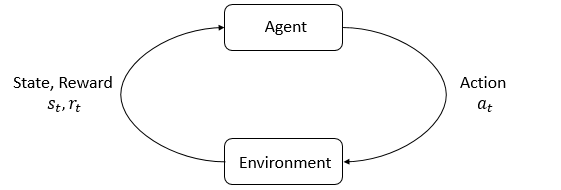
\includegraphics[width=0.64\textwidth]{reinforcement_learning_loop.png}
    \captionsetup{font=scriptsize}
    \caption{
    Diagram of Reinforcement Learning loop.
    }
    \label{fig:reinforcement_learning_loop}
\end{figure}

The general process of reinforcement learning can be expressed as follows: In an Environment, an Agent performs an Action in response to different Observations/States and then receives a corresponding Reward, adjusting its Action tendency based on the Reward.
In a recurring cycle, the Agent becomes increasingly capable of obtaining higher Rewards for given Observations/States.
If the Reward mechanism is designed reasonably, the Agent can eventually better solve the problem presented by the Environment, as shown in Figure \ref{fig:reinforcement_learning_loop}.

\subsubsection{Dynamic Mode Decomposition}\indent

Dynamic Mode Decomposition (DMD) was originally used to analyze the dynamic processes of fluids.
Simply put, flow field information at each moment can be expanded into a one-dimensional vector, and combining flow field vectors from multiple consecutive moments will yield a flow field time-series matrix.

For two flow field time-series matrices starting from adjacent moments and containing the same $m-1$ number of time nodes:

\begin{equation}\matrix{\rm\textbf{X}_{1(n\times m)} & = & [ & \rm\textbf{x}_{n\times1}(t_0) & \rm\textbf{x}_{n\times1}(t_1) & \cdot\cdot\cdot & \rm\textbf{x}_{n\times1}(t_{m-1}) & ]\cr
                        \rm\textbf{X}_{2(n\times m)} & = & [ & \rm\textbf{x}_{n\times1}(t_1) & \rm\textbf{x}_{n\times1}(t_2) & \cdot\cdot\cdot & \rm\textbf{x}_{n\times1}(t_{m}) & ]}\end{equation}

Where $\rm\textbf{x}_{n\times1}(t_{k})$ refers to the flow field information at time $k$ expanded into a vector containing information from $n$ grid points, and $\rm\textbf{X}_{1(n\times m)}$ and $\rm\textbf{X}_{2(n\times m)}$ are flow field time-series matrices obtained by combining expansion vectors from $m$ moments.

A transformation matrix exists such that:

$$\rm\textbf{X}_{2}\approx \rm\textbf{AX}_{1}$$

By solving this transformation matrix and performing eigenvalue and eigenvector analysis, researchers can determine the time evolution law of the flow field.
Since the calculation for directly inverting $\rm\textbf{X}$ can be very large, DMD actually provides a processing method that saves computational resources.
Clearly, this analysis process is not limited to flow field information.
As a purely data-driven analysis method, DMD has now been generalized and applied to a wider range of time-series analyses, such as in the field of machine learning.
Currently, many researchers have applied DMD to analyze flow field information.
Tong Zheming et al. used DMD to study the evolution mechanism of blade passage vortices in mixed-flow turbines under partial load conditions;
Zhang Wensen et al. used DMD to study the relationship between diseased arterial blood flow and wall stress;
Ge Penghui et al. analyzed the evolution of the in-cylinder flow field of a direct-injection optical engine;
Chen Jiaxing et al. analyzed the spatio-temporal distribution of sea surface temperature in the offshore area of the Yangtze River Estuary;
Xie Hairun et al. studied the phenomenon of vortex-induced vibration;
Hu Chenxing et al. studied fluid patterns in centrifugal compressor volutes;
Chen Zhenli et al. studied the transition process.
In this paper, the DMD method is applied to analyze the flow field generated by the optimized shapes obtained from the reinforcement learning algorithm to analyze the flow mechanism behind the optimized design.

\section*{Methods}
\addtocounter{section}{1}
\setcounter{subsection}{0}
\addcontentsline{toc}{section}{\protect\numberline{}Methods}\indent

\subsection{Model and Optimization Design Process of Synthetic Jet Device}\indent

The basic structure of a synthetic jet device includes three parts: vibrating membrane, chamber, and orifice. Specifically in this paper,
the model considered is shown in Figure .

\begin{figure}[htbp]
    \centering
    \begin{subfigure}[b]{0.48\textwidth}
        \centering
        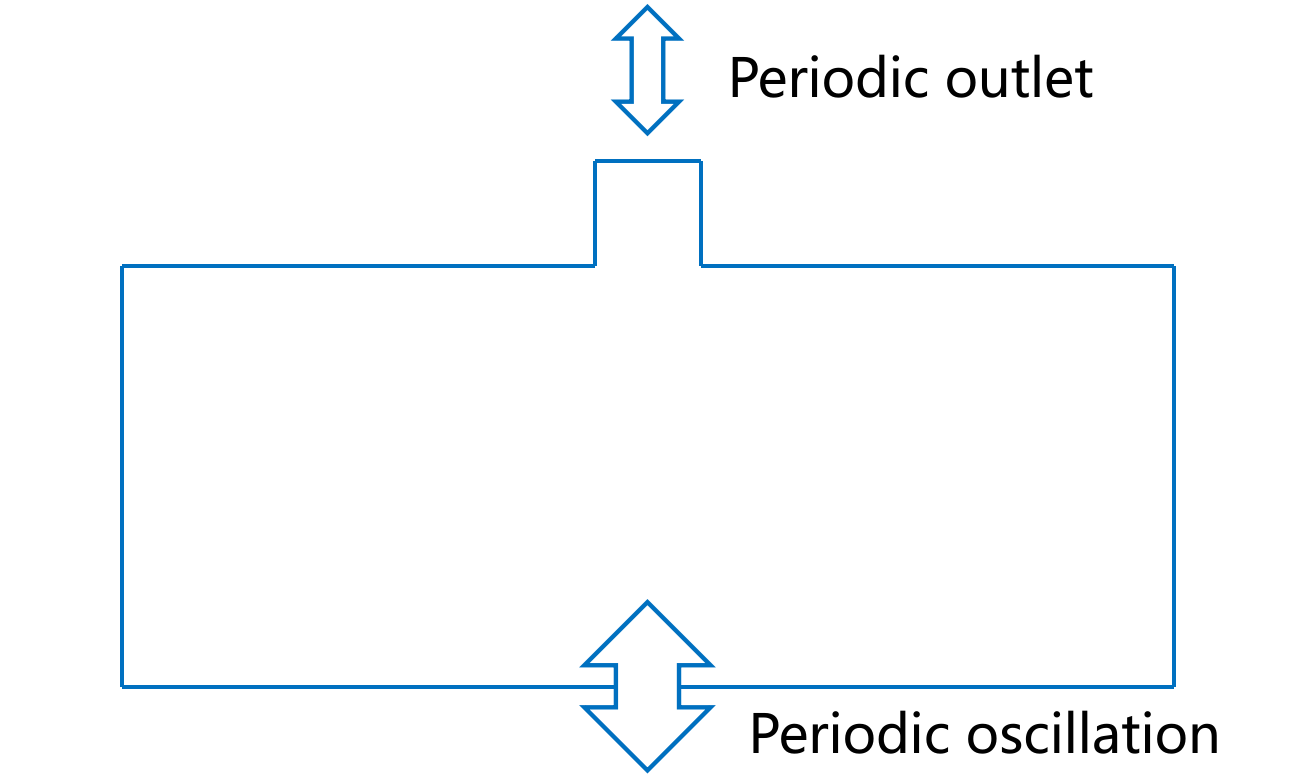
\includegraphics[width=0.96\textwidth]{synthetic_jet_diagram_periodic_oscillation.png}
        \subcaption{}
    \end{subfigure}
    \begin{subfigure}[b]{0.48\textwidth}
        \centering
        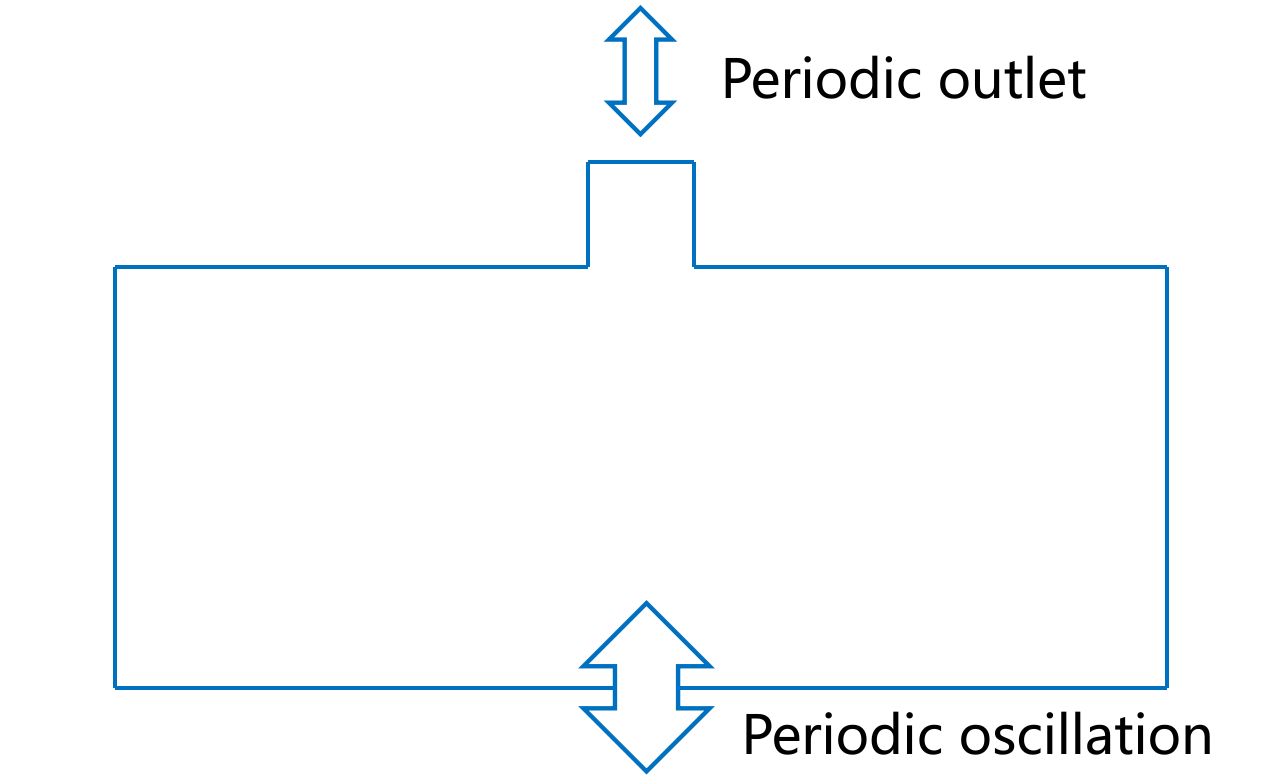
\includegraphics[width=0.96\textwidth]{synthetic_jet_diagram_periodic_velocity_inlet.png}
        \subcaption{}
    \end{subfigure}
    \captionsetup{font=scriptsize}
    \caption{
    Synthetic jet device digrams.
    (a) Considered digram.
    (b) Actual digram for calculation.
    Empirically, directly setting the jet outlet at the outlet of the boundary conditions may cause calculation distortion.
    After setting the velocity input and the jet outlet boundary conditions to non-reflective boundary conditions,
    the trial calculation results show that after adding a ``buffer zone'' with an area similar to the model above the model outlet,
    the pressure results differ by less than 5\%, the outlet velocity amplitude differs by 10\%, and the relative relationship between the data between shapes is not changed.
    }
    \label{fig:rl_diagrams}
\end{figure}

The bottom of the synthetic jet device model is a vibrating membrane, which undergoes periodic sinusoidal vibration at a certain frequency and amplitude.
Assume that the bottom diaphragm vibrates periodically according to the rule
\begin{equation}h=-\frac{A}{2\pi}{\rm cos}(2f\pi t)\end{equation}
(where $h$ refers to the displacement of the vibrating membrane, $A$ is the amplitude, and $f$ is the vibration frequency).
With the periodic vibration of the diaphragm, the fluid in the chamber is periodically pushed by positive pressure and ``drawn back'' by ``negative pressure'',
periodically passing through the outlet of the synthetic jet device (that is, the junction of the jet device and the upper pipe), and shooting or sucking fluid into the pipe.

For the numerical simulation calculation of this process, the most ideal technical implementation path is to adopt a dynamic mesh scheme to completely simulate the original physical model of synthetic jets.
The dynamic mesh setting needs to consume more calculation resources to meet the geometric constraints, and the CFD tool PyFR used in this paper currently does not support dynamic mesh settings.
Previous researchers (such as Shi Qing et al. [10]) have proven that under the two conditions of using dynamic mesh and adopting periodic velocity input boundary conditions at the corresponding positions of the vibrating diaphragm (of course, the two are in a derivative relationship with each other), the obtained flow field results match very well.

The CFD scheme used in PyFR in this paper uses a static mesh, and at the bottom of the synthetic jet chamber follows
\begin{equation}u=0, v=Af\sin(2f\pi t)\label{equation:periodic_velocity_inlet}\end{equation}
to set the velocity input at the bottom boundary.
Where $u$ refers to the velocity in the horizontal direction at the bottom velocity inlet, and $v$ is the velocity in the vertical direction.
This paper uses dimensionless parameters for calculation.
The density characteristic quantity selected is the density of water, the length characteristic quantity is the width of the outlet pipe (also referred to as the geometric unit size in this paper), and the ambient pressure is 1000 Pascals.
The viscosity coefficient and Prandtl number are set to the viscosity coefficient of water 0.001 and Prandtl number 7.56.
Specifically, this paper sets the bottom velocity inlet boundary and the upper outlet boundary type to PyFR's char-riem-inv boundary (Riemann characteristic invariant boundary condition/non-reflective boundary condition),
and the rest are set as walls; fluid density 1.0 and fluid pressure 1.0 are set in the boundary parameters and initial conditions;
the velocity at the bottom boundary is set according the Equation \ref{equation:periodic_velocity_inlet}, and the horizontal and vertical velocities at the top outlet are set to 0. Subsequent
calculation results are all dimensionless.

Empirically, directly setting the boundary condition outlet at the jet outlet may cause calculation distortion.
Trial calculations show that PyFR's char-riem-inv boundary (Riemann characteristic invariant boundary condition/non-reflective boundary condition) has good robustness.
This paper once added a ``buffer zone'' with an area similar to the model above the model,
and found through comparison that the pressure results with and without the ``buffer zone'' differ by less than 5\%, and the outlet velocity amplitude differs by approximately 10\%,
and these differences will not change the relative relationship of data between different shapes.

\subsection{Optimization Goals and Optimization Design Variables}\indent

As introduced in the introduction part, researchers have tried to apply synthetic jets to various scenarios, especially in the direction of flow control.
During the working process of a synthetic jet device, the fluid in the chamber needs to be continuously ``gathered'' to a narrow outlet,
and the internal fluid movement is inevitably intense. In order to interact and couple with the macroscopic flow and play an effective adjustment role,
the synthetic jet device must provide jets that meet certain requirements for velocity and frequency.
This will cause the chamber of the synthetic jet device to bear relatively large pressure during the working process.
The basic starting point of this paper is to hope that while ensuring the amplitude of the synthetic jet outlet velocity (trial results show that the frequency is basically consistent with the frequency of the periodic velocity input at the bottom),
the pressure on the chamber wall is reduced.
For this purpose, some optimization goals are selected: pressure integral $p_{integral}$ along the wall ($p$ is the pressure on the wall point) and maximum pressure $p_{max}$,
as well as the outlet velocity amplitude $\Delta v$ as a guarantee item ($v$ refers to the longitudinal velocity at a point at the outlet,
the specific position is shown in Figure \ref{fig:reference_shapes},
\begin{equation}\Delta v = v_{max} - v_{min}\end{equation}
Based on some rough experience and preliminary trial calculations of several examples, it is noticed that even without changing other parameters,
changing the chamber shape can have a significant impact on the flow field.
Representatively, the wall pressure integral, wall maximum pressure, and outlet velocity amplitude data under the rectangular chamber shape and trapezoidal chamber shape (Figure \ref{fig:reference_shapes}) under the same physical parameters are given here (Table \ref{tab:pressure_and_outlet_velocity_data_of_references}).
The approximate position of the outlet velocity sampling point is marked with a circle (that is, the central point of the outlet channel. Subsequent outlet velocity sampling points all use the same position and will not be repeated).

\begin{table}[h]
    \centering
    \caption{Pressure and outlet velocity data of references}
    \label{tab:pressure_and_outlet_velocity_data_of_references}
    \begin{tabular}{c c c c}
        \hline
        \hline
        &{Wall pressure integral}&{Wall maximum pressure}&{Outlet velocity amplitude}\\
        \hline
        {Rectangular}&{3.698828}&{1.311709}&{0.416794}\\
        \hline
        {Trapezoidal}&{2.608055}&{1.479009}&{0.820818}\\
        \hline
        \hline
    \end{tabular}
\end{table}

\begin{figure}[htbp]
    \centering
    \begin{subfigure}[b]{0.48\textwidth}
        \centering
        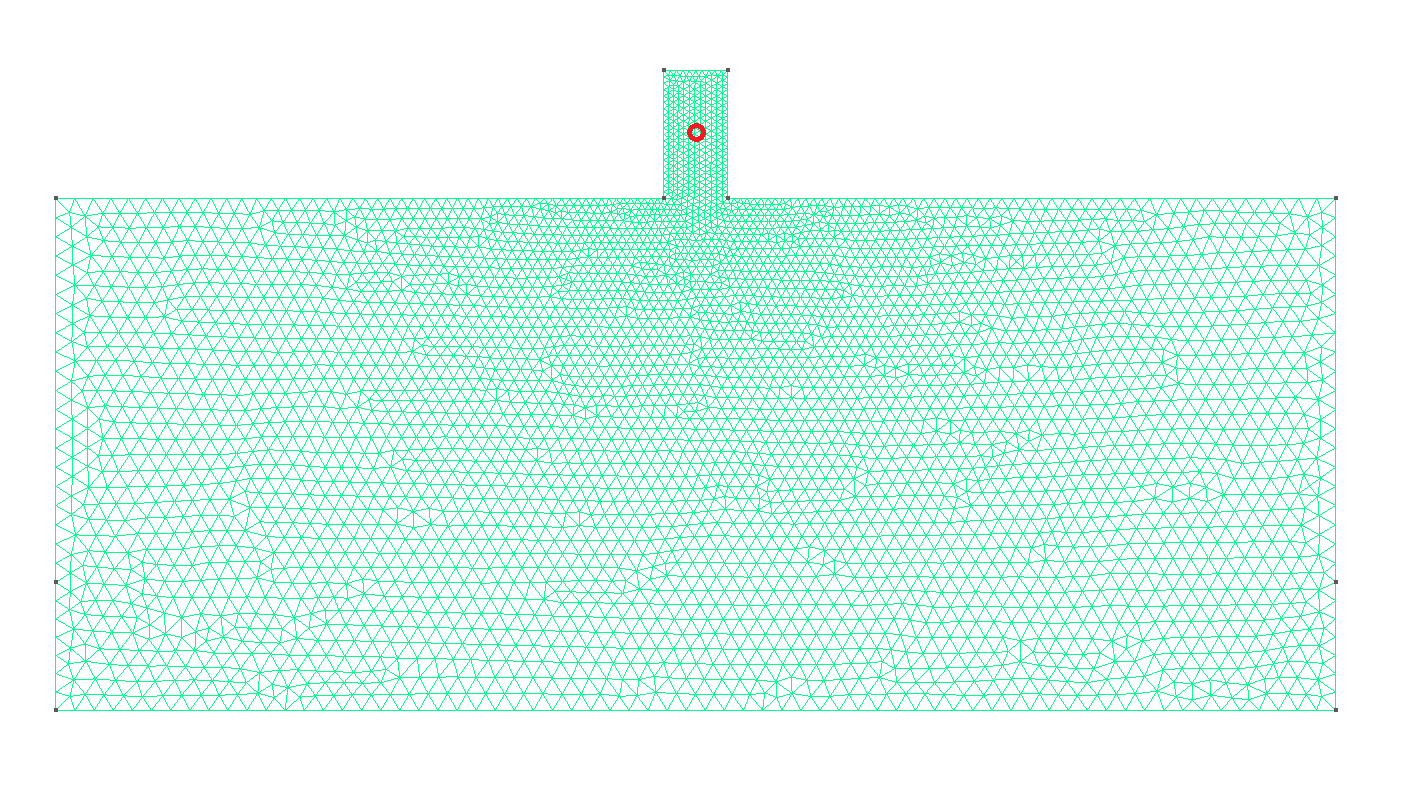
\includegraphics[width=0.96\textwidth]{reference_shape_rectangular.png}
        \subcaption{}
    \end{subfigure}
    \begin{subfigure}[b]{0.48\textwidth}
        \centering
        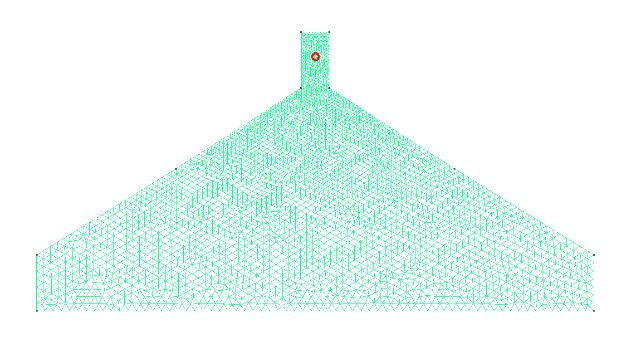
\includegraphics[width=0.96\textwidth]{reference_shape_trapezoidal.png}
        \subcaption{}
    \end{subfigure}
    \captionsetup{font=scriptsize}
    \caption{
    Reference shapes.
    (a) Rectangular chamber mesh used in the trial calculation (including 7879 triangular elements) and (b) trapezoidal chamber mesh (including 5563 triangular elements).
    The red circle is the specific position where outlet velocity data is collected (center point of the outlet channel).
    }
    \label{fig:reference_shapes}
\end{figure}

These two chamber shapes have two things in common:
1. They are bilaterally symmetrical;
2. The chamber wall curve can be seen as starting from the bottom and top endpoints, through two ``control points'' at the upper left and upper right, connected using polylines to reach the upper outlet endpoints.
Keeping this ``control point + connecting curve'' mode unchanged, given a certain number of control points, adjust the position of the control points and use a certain type of curve
(such as Spline spline curve, BSpline/B-spline curve, Bezier/Bezier curve, etc.) to connect the endpoints and these control points to each other to obtain different chamber shapes.
A specific training in this paper will first give the number of control points, and then use the reinforcement learning algorithm to adjust the position of the control points to change the chamber shape.

The final optimization idea of this paper can be expressed as: under the same bottom periodic velocity input, same chamber height, same outlet channel, and same connecting curve type,
with the preset chamber shape being bilaterally symmetrical, and given the number of control points, use the reinforcement learning algorithm to automatically adjust the control point coordinates and the shape of the synthetic jet chamber,
while ensuring the amplitude of the outlet velocity, the pressure on the chamber wall is reduced (specifically the wall pressure integral and the maximum pressure on the wall; this paper pays more attention to the maximum pressure on the wall).
The next section will specifically introduce how the reinforcement learning algorithm adjusts the position of the control points and how the optimization goals of concern are reflected in the Reward calculation of reinforcement learning.

\subsection{Reinforcement Learning Automatic Optimization Process}\indent

In the design of this paper, the Agent in reinforcement learning selects numerical values in a multi-dimensional continuous space,
these data correspond to different control point coordinates, different chamber shapes, and different optimization target data.
Specifically, in the reinforcement learning Environment designed in this paper, an Action Space (multi-dimensional continuous space) is set,
which actually corresponds to the range of abscissas and ordinates of one or more control points (as shown in Figure \ref{fig:control_point_range}).
No relationship is manually preset between the coordinates.
Each Action made by the Agent is taking a value in each dimension to form a one-dimensional vector,
corresponding to the relevant coordinates and chamber shape, and then a Reward calculated for this chamber shape is given.

\begin{figure}[htbp]
    \centering
    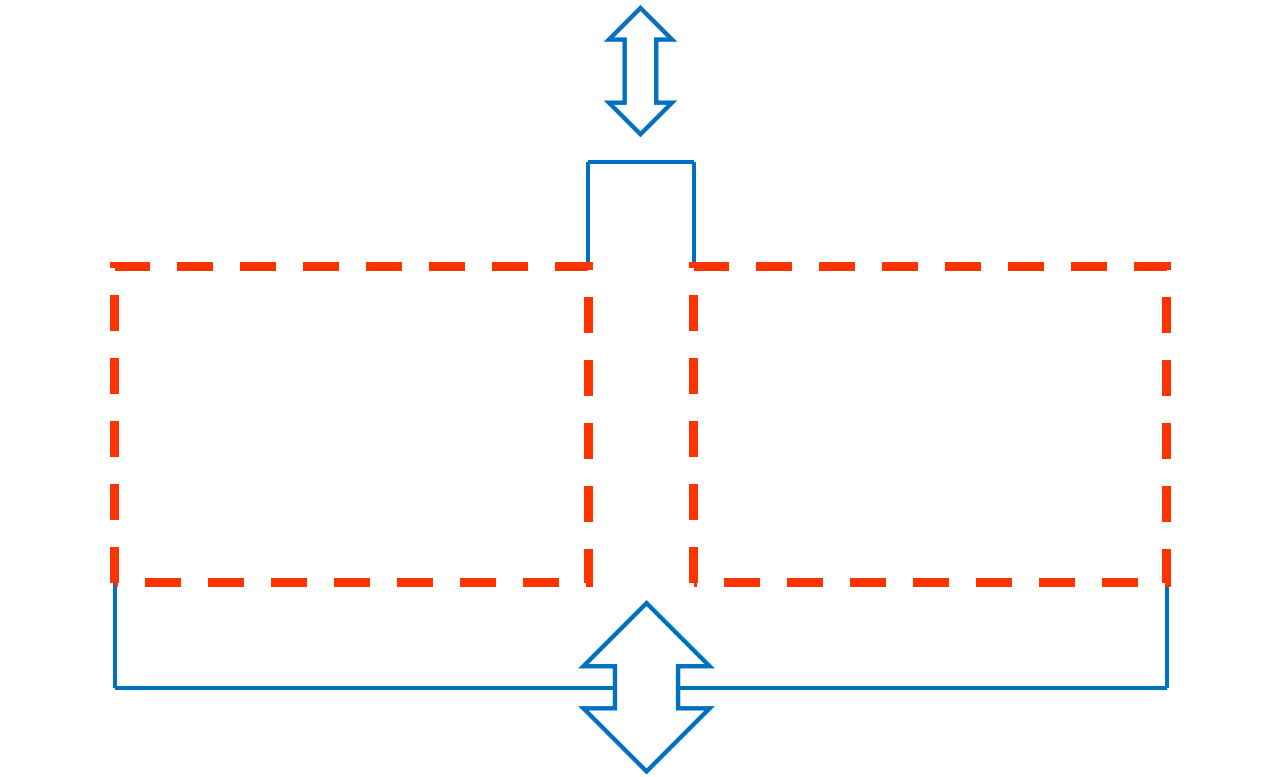
\includegraphics[width=0.64\textwidth]{control_point_range.png}
    \captionsetup{font=scriptsize}
    \caption{
    The range of movement of each control point corresponding to the set Action Space, and no relationship between control points is preset.
    }
    \label{fig:control_point_range}
\end{figure}

In order to ensure that when the Agent picks a control point position whose ordinate is very close to the bottom edge, the mesh can be generated normally and effectively, this paper added a segment at the bottom.
When calculating wall-related data, only the part of the chamber wall corresponding to the spline curve generated by the endpoints and control points is considered.
Taking the case of three control points as an example, an Action made by the Agent is a one-dimensional vector containing six elements.

After a simple linear transformation (reinforcement learning algorithms usually need to normalize each dimension of the Action Space to a continuous space of [-1,1] to satisfy the Gaussian distribution), it is converted into the horizontal/vertical coordinates of the three points.
Then the obtained control point coordinates are passed into the physical calculation function, and PyFR and self-written post-processing programs are called.
Based on a stable cycle, the wall pressure integral, wall maximum pressure, and outlet velocity amplitude are obtained.
Then the Reward value is calculated based on these data according to the set algorithm and fed back to the Agent.
The Agent adjusts ``its own'' ``behavioral tendency'' based on the obtained Reward, and then starts a new round of attempts and training.
The specific flow chart is shown in Figure \ref{fig:reinforcement_learning_optimization_procedures}.

\begin{figure}[htbp]
    \centering
    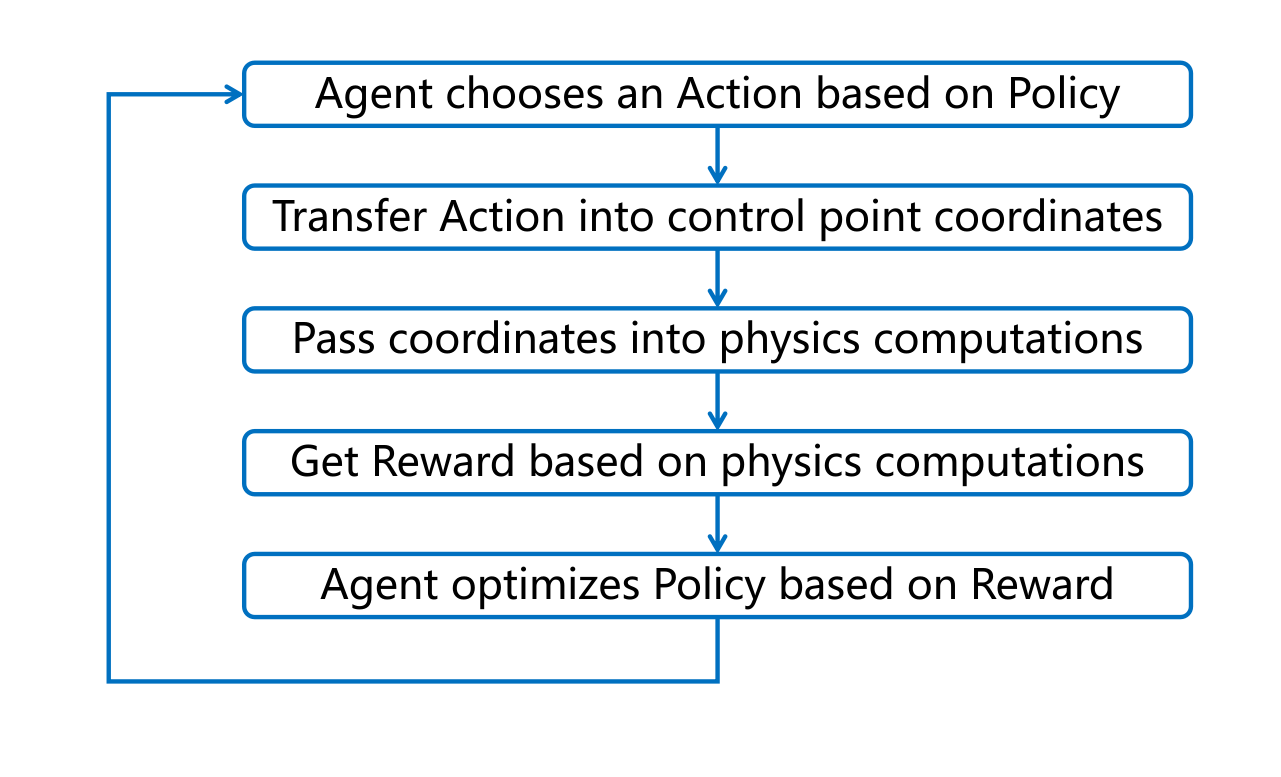
\includegraphics[width=0.64\textwidth]{reinforcement_learning_optimization_procedures.png}
    \captionsetup{font=scriptsize}
    \caption{
    Diagram of Reinforcement Learning optimization procedures.
    }
    \label{fig:reinforcement_learning_optimization_procedures}
\end{figure}

As mentioned when introducing the CartPole example above, in this paper, Actions are not taken in response to changing Observations,
but attempts are repeatedly made for a fixed Observation and a fixed problem to obtain superior solutions.
The significance of Observation in this paper is not as obvious as in a general reinforcement learning Environment.
The application method of reinforcement learning in this paper has its own characteristics.

\begin{figure}[htbp]
    \centering
    \begin{subfigure}[b]{0.32\textwidth}
        \centering
        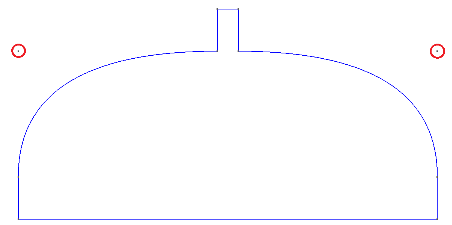
\includegraphics[width=0.96\textwidth]{example_chamber_shape_b_spline.png}
        \subcaption{}
    \end{subfigure}
    \begin{subfigure}[b]{0.32\textwidth}
        \centering
        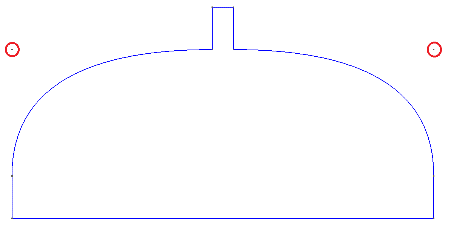
\includegraphics[width=0.96\textwidth]{example_chamber_shape_bezier.png}
        \subcaption{}
    \end{subfigure}
    \begin{subfigure}[b]{0.32\textwidth}
        \centering
        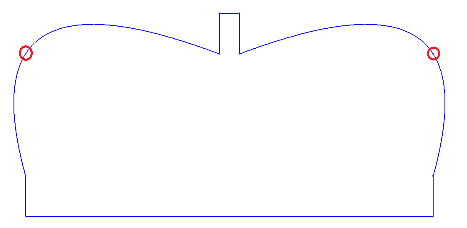
\includegraphics[width=0.96\textwidth]{example_chamber_shape_spline.png}
        \subcaption{}
    \end{subfigure}
    \captionsetup{font=scriptsize}
    \caption{
    Example chamber shape of curves.
    Examples of chamber shapes generated by (a) B-spline curves, (b) Bezier curves, and (c) spline curves under the same control points.
    Spline curves can better reflect the influence of control points on the chamber shape and were selected for this paper.
    }
    \label{fig:example_chamber_shape_of_curves}
\end{figure}

During the trial calculation process, the influence of the connecting curve type on the chamber shape was noticed. This paper used the mesh generation tool
Gmsh and its Python API version PyGmsh's built-in Bezier, BSpline, and
Spline. Under the same point coordinate settings, the shapes obtained by Bezier curves and B-spline curves are similar,
and the smoothness is significantly higher than that of spline curves (Figure \ref{fig:example_chamber_shape_of_curves}). But these two types of curves do not necessarily pass through the control points.
In other words, the influence of control point coordinates on the curve will be buffered under these two types of curves.
Ordinary spline curves pass through control points and cannot achieve very good smooth fitting performance, but can better reflect
the influence of control points on the curve shape.
Finally, this paper chose ordinary spline curves to generate chamber curves.

To limit the behavior of the Agent as little as possible, provide a large enough range of control point movement as much as possible,
do not preset the relationship between control points as much as possible, and hope to reflect the influence of control points on the chamber shape as much as possible.
The Agent will inevitably try some special control point coordinates during the training process, resulting in the mesh generation and post-processing not necessarily being completed normally.
Cases of special control point coordinates will appear in large numbers in the early stage of training.

Therefore, in the program design of this paper, the robustness design of the physical calculation part played an important role.
In this paper, the encapsulated physical calculation program can be divided into three parts: 1. Mesh preparation: generate the required
mesh file and convert it into the pyfrm format supported by PyFR; 2. Physical calculation: read the previously generated mesh and the previously
prepared physical configuration information file, call PyFR to complete the physical calculation, and save the original flow field information file; 3. Use
self-written programs to read the original flow field information file saved by PyFR, extract grid point data of the boundary and outlet parts at
multiple moments in a cycle, calculate the pressure integral, maximum pressure, outlet
velocity and other data for each moment, and take the maximum values of the pressure integral and maximum pressure of these moments and the
range of the outlet velocity as the final considered values.

It is hoped that when the Agent tries an unreasonable shape and fails to complete the three parts of the physical calculation normally, it
can learn the error and make the next attempt. If a shape cannot normally go through the physical calculation process, it is highly
unlikely to be the desired shape, and the corresponding Reward is assigned a negative value. For chamber shapes
that can complete the physical calculation process, their outlet velocity performance must also be judged.
Only those that meet the outlet velocity performance requirements will truly enter the Reward calculation based on wall pressure integral, wall maximum pressure, and outlet velocity amplitude;
otherwise, Reward is assigned as 0.
Examples of ``problematic shapes'' and specific processes are shown in Figure \ref{fig:robustness_design}.

\begin{figure}[htbp]
    \centering
    \begin{subfigure}[b]{0.48\textwidth}
        \centering
        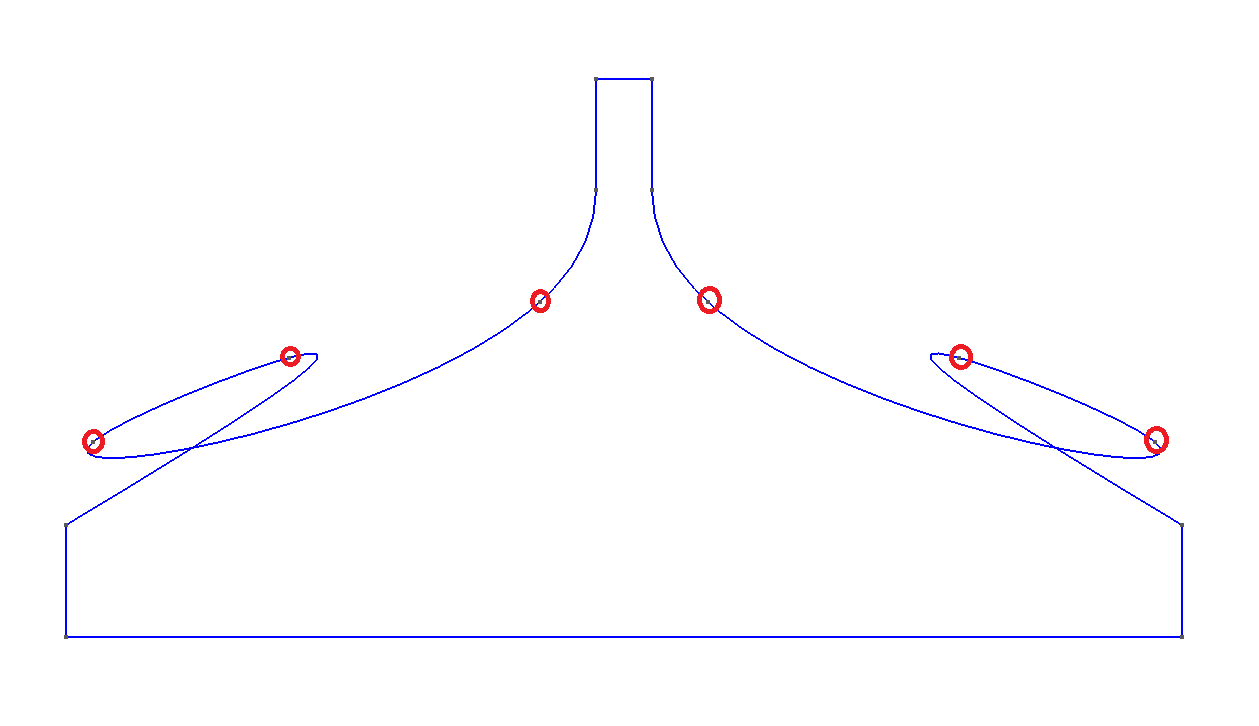
\includegraphics[width=0.96\textwidth]{problematic_camber_shape_example.png}
        \subcaption{}
    \end{subfigure}
    \begin{subfigure}[b]{0.48\textwidth}
        \centering
        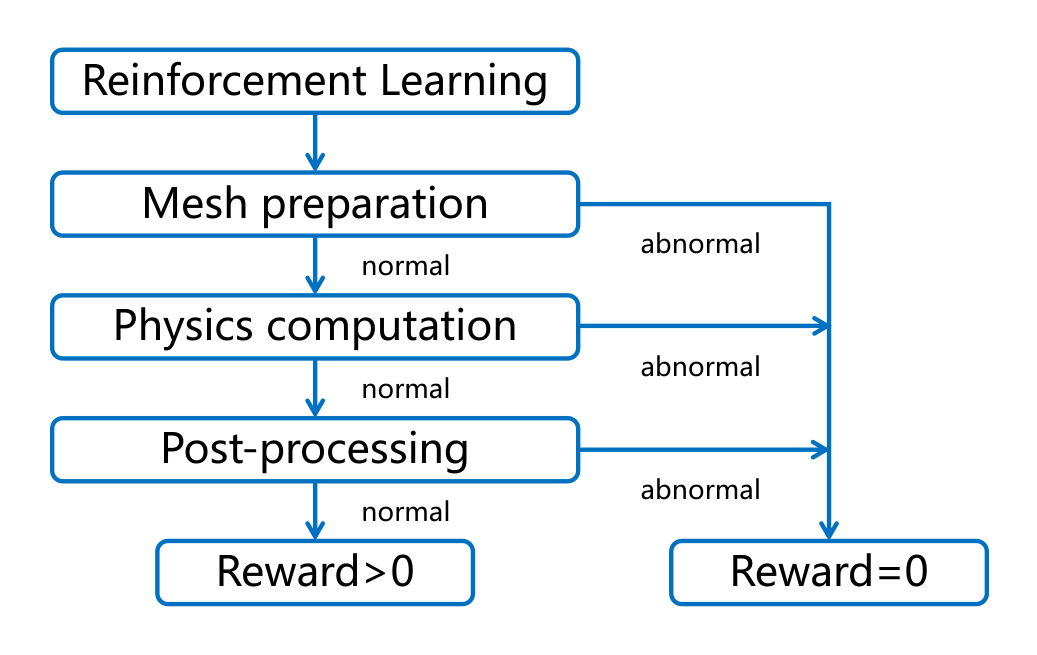
\includegraphics[width=0.96\textwidth]{robustness_design.png}
        \subcaption{}
    \end{subfigure}
    \captionsetup{font=scriptsize}
    \caption{
    Robustness design.
    (a) Example of ``problematic shape''; (b) Robustness design of physical functions and its influence on Reward.
    Giving the Agent as much freedom as possible for the control point range and do not limit the relationship between control points.
    Thus, a robust design must be done.
    }
    \label{fig:robustness_design}
\end{figure}

Under such robustness design, the reinforcement learning model will continue training regardless of whether the physical calculation is completed normally.
This achieves weak control over the Agent's behavior and minimizes human influence on the Agent's Action.

Finally, a brief introduction to the basic setting idea of the Reward function is provided.

For each Case, this paper first manually presets a shape and calculates its corresponding wall pressure integral, maximum wall pressure, and outlet velocity amplitude.
Three benchmark values are set based on these data.
The differences between subsequent calculated wall pressure integrals, maximum wall pressures, and outlet velocity amplitudes and these benchmark values are multiplied by their respective coefficients, summed, and then added to a benchmark constant to obtain the final Reward value.
The addition of a Reward benchmark constant is necessary to prevent the Agent from finding it difficult to obtain a (positive value) Reward in early attempts.
A specific reinforcement learning training session will always consider the outlet velocity amplitude, and additionally, one can choose to consider only the wall pressure integral, only the maximum wall pressure, or both simultaneously.
The wall pressure integral is related to the length of the wall curve and does not fully reflect pressure characteristics.
This paper focuses more on the two quantities: maximum wall pressure and outlet velocity amplitude.

During the process where the Agent of the reinforcement learning algorithm makes attempts and optimizes based on the designed Reward algorithm, it will inevitably favor either pressure or velocity performance, even if not obviously.
It was noted during trial calculations that there seems to be a complex coupling relationship between the wall pressure integral, maximum pressure, and outlet velocity amplitude.
It is difficult to optimize one parameter without affecting the performance of the other two factors, and it is difficult to optimize multiple data points together.

Therefore, this paper does not only focus on the chamber shape with the highest Reward but also considers shapes with the next-best Reward,
to avoid the optimization work falling into a local optimum and ignoring other possibilities, much like the reinforcement learning algorithm itself.

\section*{Results}
\addtocounter{section}{1}
\setcounter{subsection}{0}
\addcontentsline{toc}{section}{\protect\numberline{}Results}\indent

\subsection{Physical Parameters and Classification of Optimization Designs}\indent

Following the process and logic described in Methods, this paper conducts optimization designs under a total of 9 different physical parameters (see Figure \ref{fig:parameters_in_the_model} and Table \ref{tab:considered_parameter_sets}).
The frameworks and algorithms used include Stable-Baselines3, A3C, PPO, TD3, and SAC.
The physical parameters of focus include geometric unit size $d$, relative chamber height $h$, diaphragm amplitude $A$, and vibration frequency $f$.
The actual velocity input amplitude is the product of the diaphragm amplitude $A$ and the vibration frequency $f$.
This study does not discuss the algorithms in detail, as the choice of reinforcement learning algorithm did not show a significant impact on the optimization results.

\begin{figure}[htbp]
    \centering
    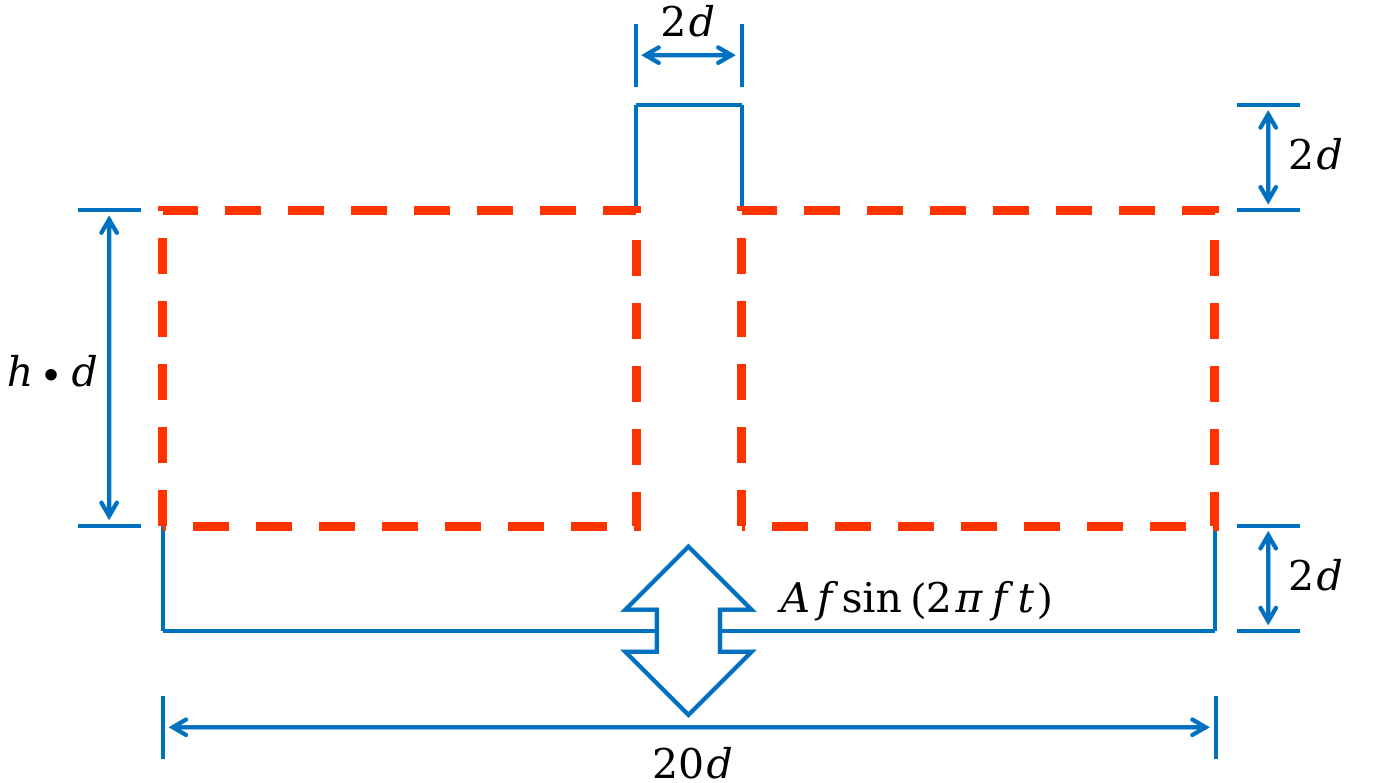
\includegraphics[width=0.64\textwidth]{parameters_in_the_model.png}
    \captionsetup{font=scriptsize}
    \caption{
    Parameters in the model.
    Meaning of relevant parameters involved in the model, including geometric unit size $d$, relative chamber height $h$, diaphragm amplitude $A$, and vibration frequency $f$.
    }
    \label{fig:parameters_in_the_model}
\end{figure}

\begin{table}[h]
    \centering
    \caption{Considered parameter sets}
    \label{tab:considered_parameter_sets}
    \begin{tabular}{c c c c c c}
        \hline
        \hline
        {Case}&{$d$}&{$h$}&{$A$}&{$f$}&{$Af$}\\
        \hline
        {0}&{1.0}&{6.0}&{1.6}&{0.50}&{0.8}\\
        \hline
        {1}&{1.0}&{3.0}&{1.6}&{0.50}&{0.8}\\
        \hline
        {2}&{1.0}&{12.0}&{1.6}&{0.50}&{0.8}\\
        \hline
        {3}&{1.0}&{6.0}&{0.8}&{0.50}&{0.4}\\
        \hline
        {4}&{1.0}&{6.0}&{3.2}&{0.50}&{1.6}\\
        \hline
        {5}&{1.0}&{6.0}&{1.6}&{0.25}&{0.4}\\
        \hline
        {6}&{1.0}&{6.0}&{1.6}&{1.00}&{1.6}\\
        \hline
        {7}&{0.5}&{6.0}&{3.2}&{0.50}&{1.6}\\
        \hline
        {8}&{2.0}&{6.0}&{0.8}&{0.50}&{0.4}\\
        \hline
        \hline
    \end{tabular}
\end{table}

Due to computational resource limitations, this paper did not attempt optimization designs using a large number of control points.
Relatively sufficient training was conducted under Case 0, attempting 1-4 control points.
Under other cases, generally 1-2 control points were attempted (the ``attempts'' for each case underwent multiple training sessions).

\subsection{Multiple Optimization Designs of Case 0}\indent

The optimized shapes obtained under Case 0 can be classified into three categories: ``Inverted T-shape'', ``S-shape'', and ``Inverted V-shape'', as shown in Figure \ref{fig:optimized_shapes_case_0}.
The ``Inverted V-shape'' is the shape pre-set to provide basic data for the Reward calculation expression.
The ``Inverted T-shape'' mainly appears in cases with 1-2 control points, while the ``S-shape'' appears in cases with 2-3 control points.
The ``Inverted V-shape'' rarely appeared during the actual optimization process.
An attempt to explain why the ``Inverted V-shape'' rarely appeared is made at the end of this section.

\begin{figure}[htbp]
    \centering
    \begin{subfigure}[b]{0.32\textwidth}
        \centering
        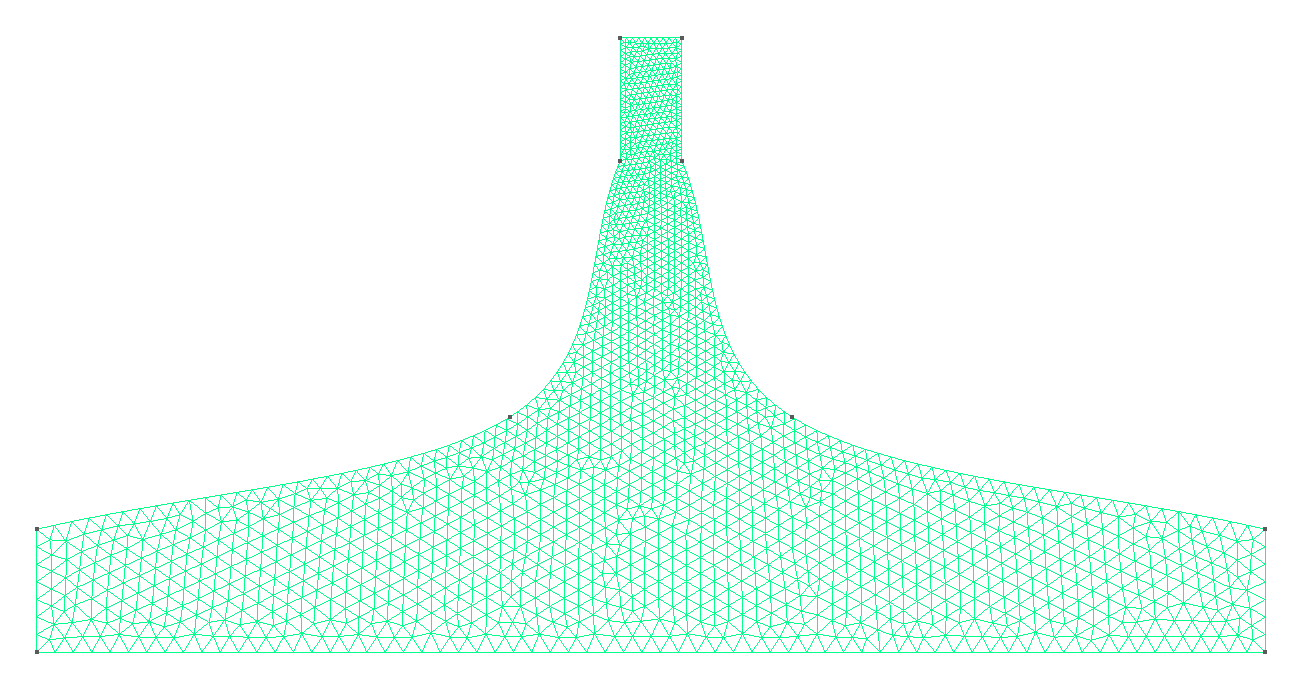
\includegraphics[width=0.96\textwidth]{optimized_shape_case_0_inverted_t.png}
        \subcaption{}
    \end{subfigure}
    \begin{subfigure}[b]{0.32\textwidth}
        \centering
        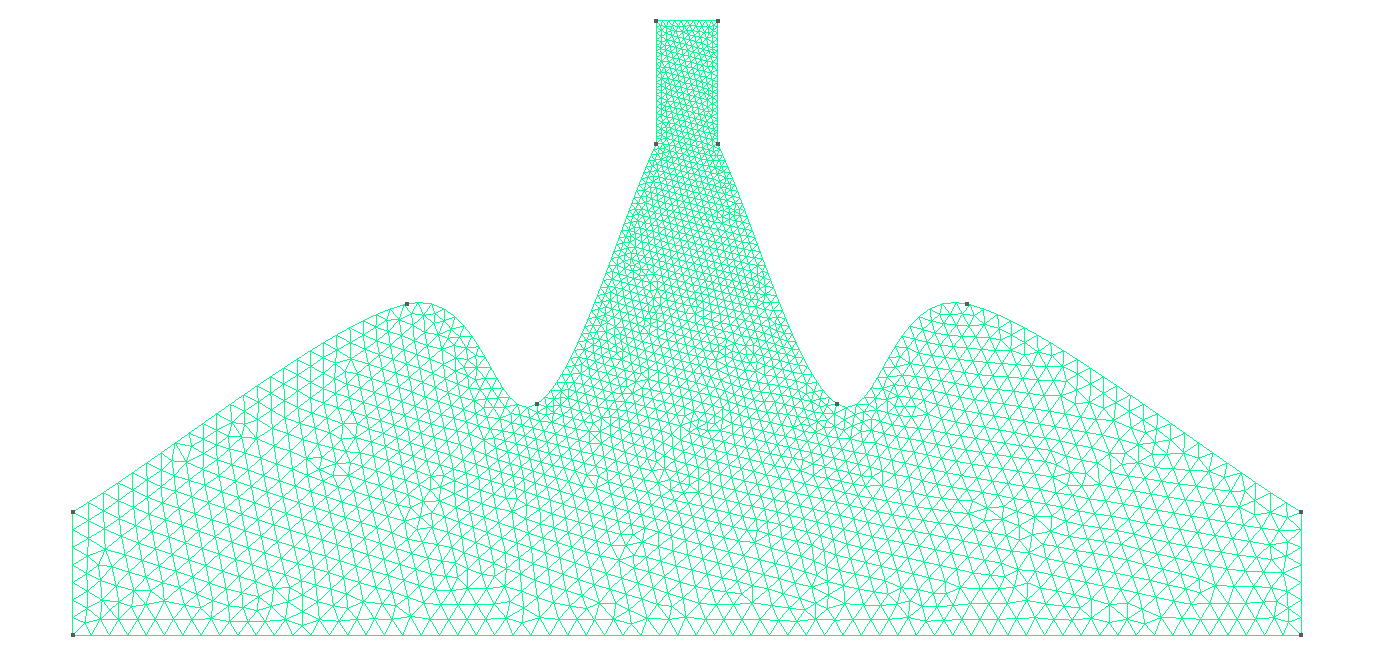
\includegraphics[width=0.96\textwidth]{optimized_shape_case_0_s.png}
        \subcaption{}
    \end{subfigure}
    \begin{subfigure}[b]{0.32\textwidth}
        \centering
        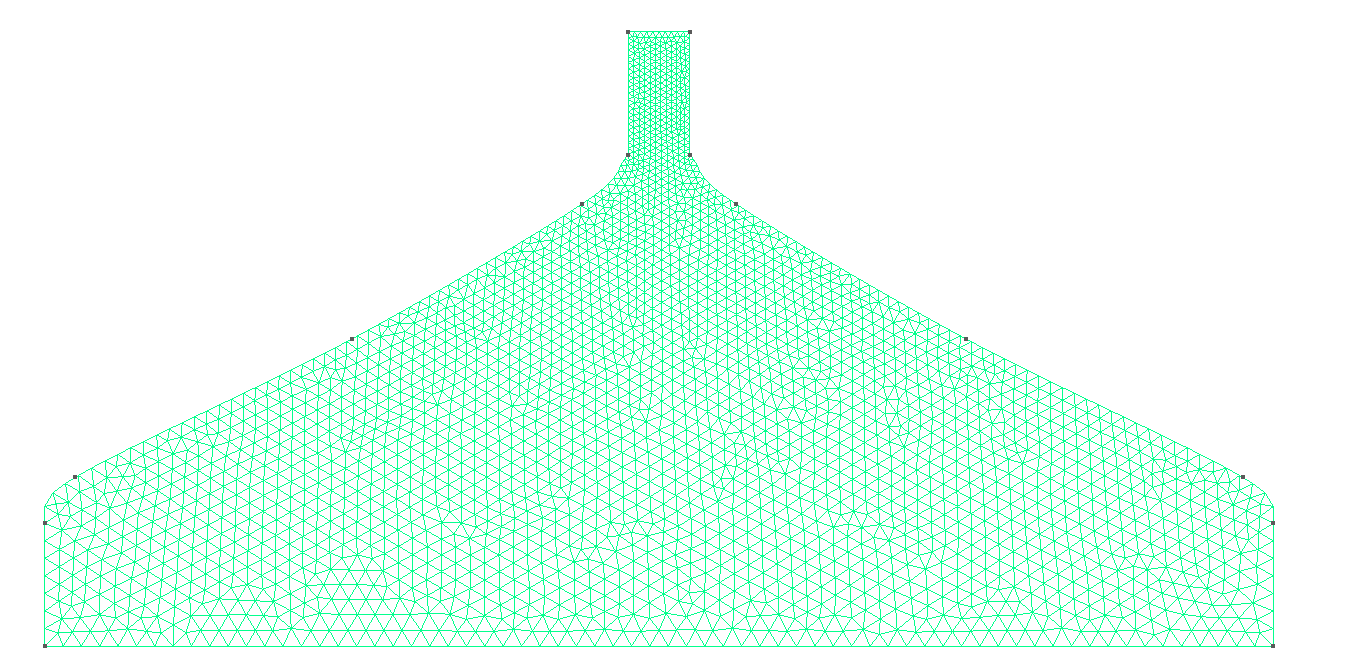
\includegraphics[width=0.96\textwidth]{optimized_shape_case_0_inverted_v.png}
        \subcaption{}
    \end{subfigure}
    \captionsetup{font=scriptsize}
    \caption{
    Three types of optimized shapes obtained under Case 0.
    (a) ``Inverted T-shape'' chamber.
    (b) ``S-shape'' chamber.
    (c) ``Inverted V-shape'' chamber.
    In practice, the frequency of ``Inverted T-shapes'' and ``S-shapes'' is significantly higher than that of ``Inverted V-shapes". 
    }
    \label{fig:optimized_shapes_case_0}
\end{figure}

Derivative shapes may be generated for ``Inverted T-shapes'' and ``S-shapes'' when more control points are used, as shown in Figure \ref{fig:optimized_shapes_derivative_case_0}.

\begin{figure}[htbp]
    \centering
    \begin{subfigure}[b]{0.32\textwidth}
        \centering
        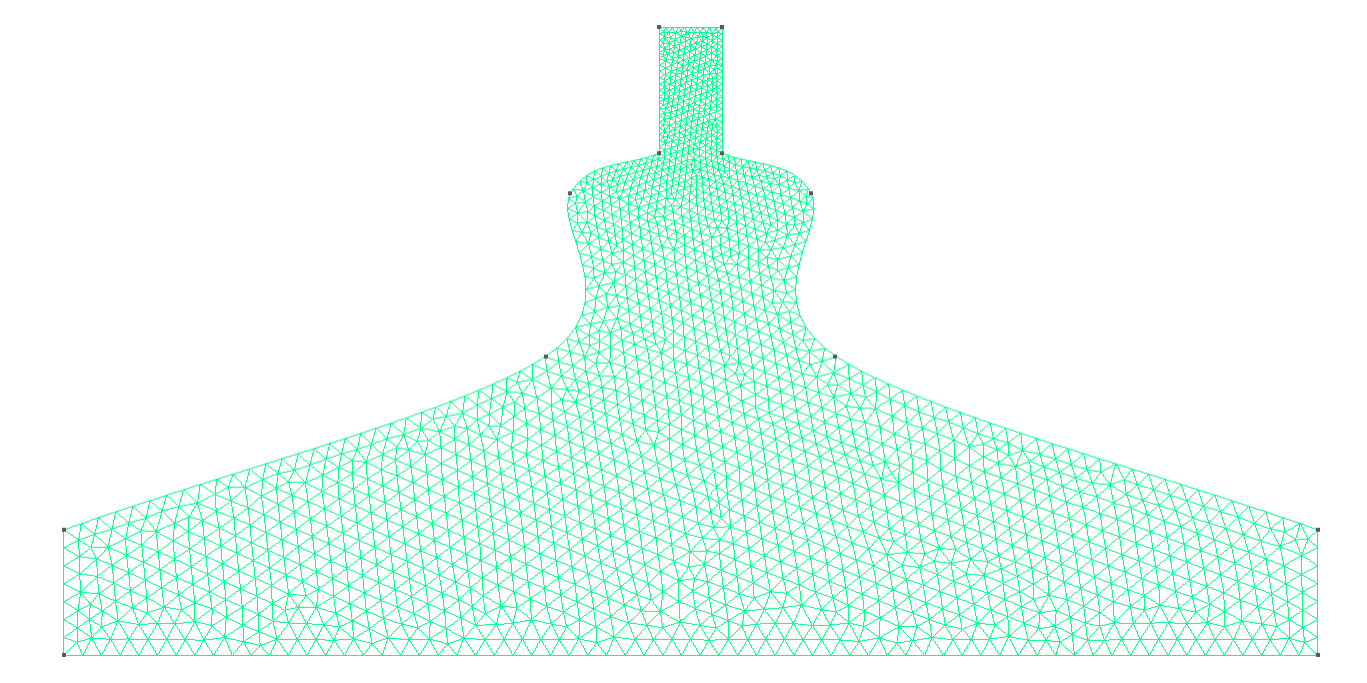
\includegraphics[width=0.96\textwidth]{optimized_shape_case_0_inverted_t_derivative.png}
        \subcaption{}
    \end{subfigure}
    \begin{subfigure}[b]{0.32\textwidth}
        \centering
        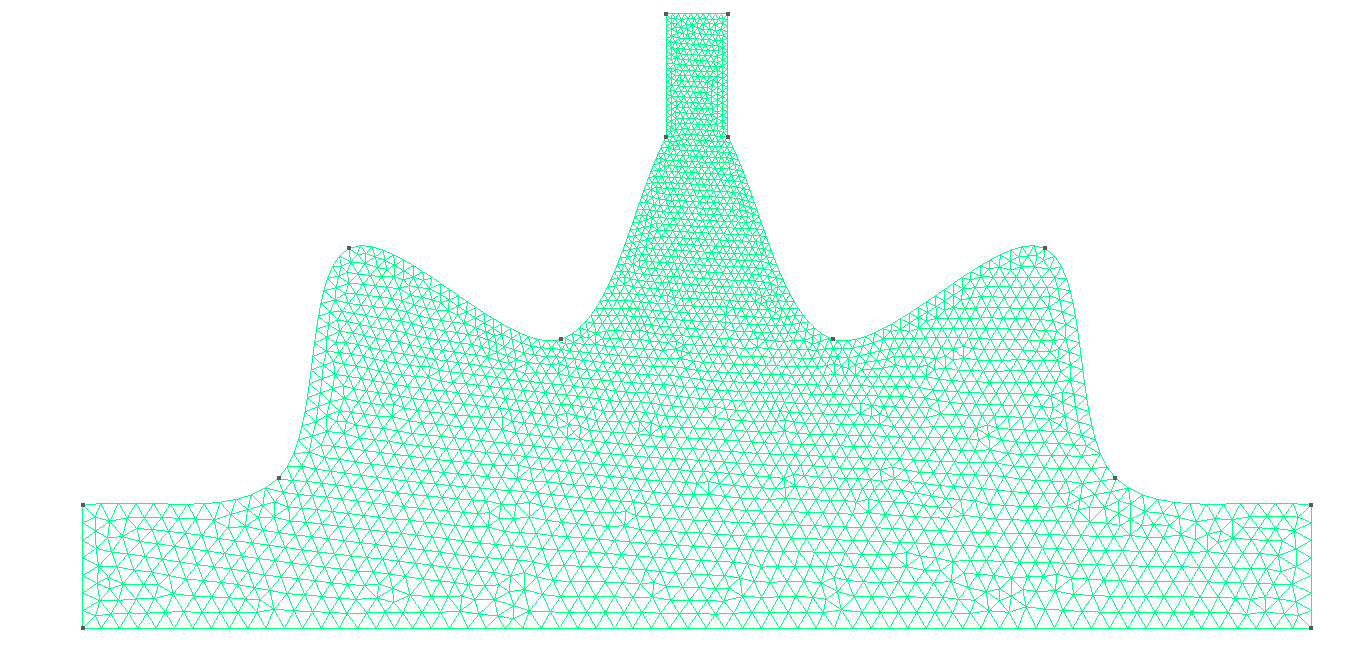
\includegraphics[width=0.96\textwidth]{optimized_shape_case_0_s_derivative.png}
        \subcaption{}
    \end{subfigure}
    \captionsetup{font=scriptsize}
    \caption{
    Derived shapes obtained under Case 0 using more control points.
    (a) Derived ``Inverted T-shape".
    (b) Derived ``S-shape". 
    }
    \label{fig:optimized_shapes_derivative_case_0}
\end{figure}

Due to the similarity between ``Inverted T-shapes'' and ``Inverted V-shapes'', shapes with good performance lying between the two were also observed.
This is also reflected under other physical parameters, but since these intermediate shapes perform similarly to the two main types, they are not listed.
The ``Inverted V-shape'' shown in Figure \ref{fig:optimized_shapes_case_0} is a pre-set shape using three control points, which almost never appeared in actual training.
"Simplified'' versions were seen when using 1 or 2 control points, especially when the optimization goal was the wall pressure integral.
These approximate shapes are close to the trapezoidal chamber shape and are not listed.

Before analyzing the principles behind these shapes, an ``Arched'' chamber shape (Figure \ref{fig:reference_shape_arched}) is provided as a reference.
This arched shape was manually selected (and was also obtained in trial calculations focusing solely on maximum wall pressure)
Additionally, the ``Rectangular'' and ``Trapezoidal'' data in Figure \ref{fig:reference_shapes} were also calculated under Case 0.

\begin{figure}[htbp]
    \centering
    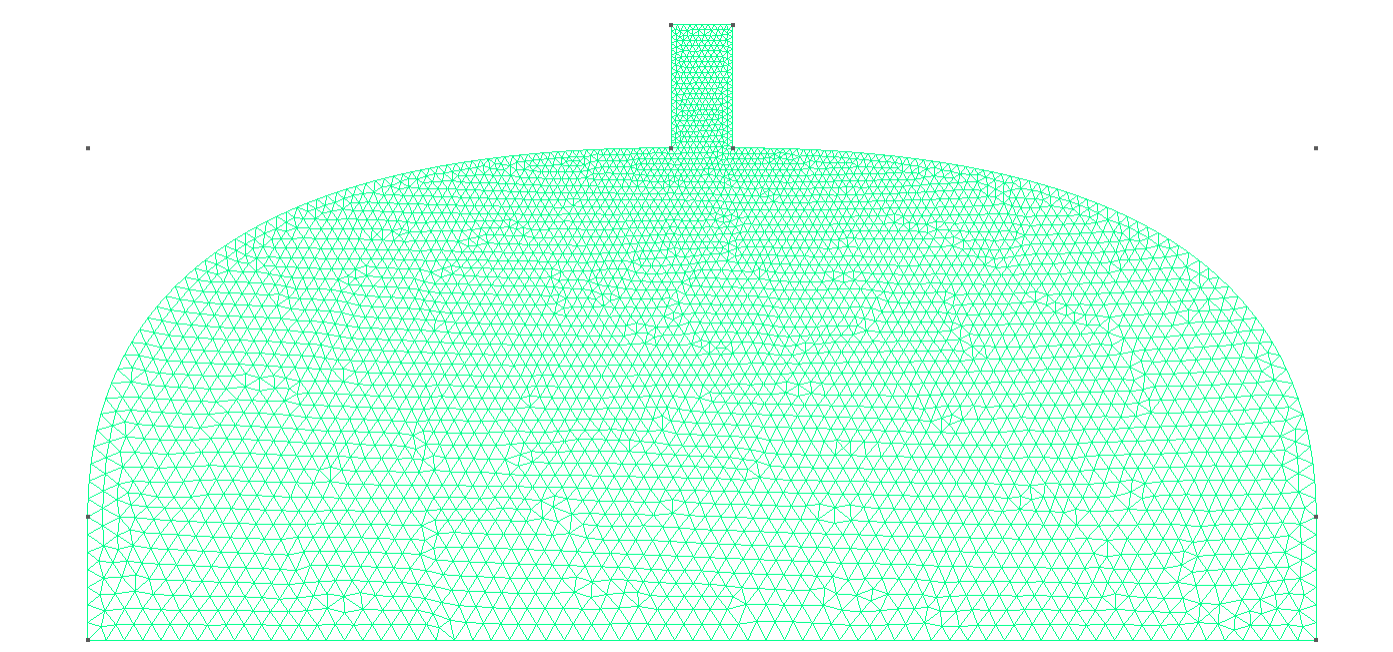
\includegraphics[width=0.64\textwidth]{reference_shape_arched.png}
    \captionsetup{font=scriptsize}
    \caption{
    Reference arched shape.
    }
    \label{fig:reference_shape_arched}
\end{figure}

Figure \ref{fig:target_data_of_optimized_shapes_case_0} shows the wall pressure integral, maximum wall pressure, and exit velocity amplitude (hereafter referred to as optimization target data) corresponding to these Case 0 chamber shapes.

\begin{figure}[htbp]
    \centering
    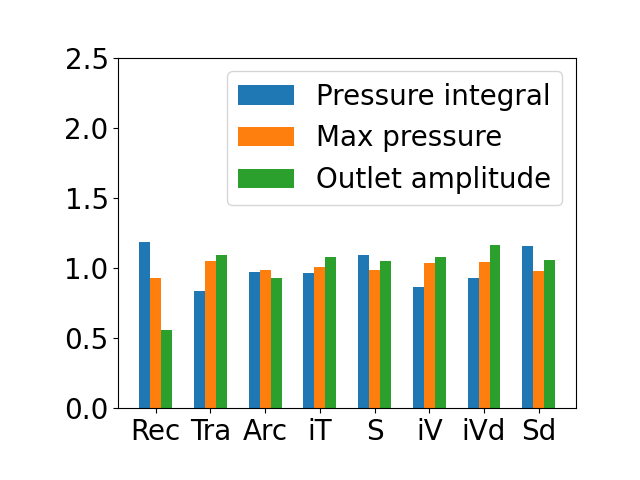
\includegraphics[width=0.64\textwidth]{target_data_case_0.png}
    \captionsetup{font=scriptsize}
    \caption{
    Target data for optimized shapes under Case 0.
    The data presented in the chart has been normalized to relative values based on their respective means.
    The various optimized shapes obtained are very close in performance regarding maximum wall pressure and exit velocity amplitude;
    they show advantages over rectangular and arched shapes.
    }
    \label{fig:target_data_of_optimized_shapes_case_0}
\end{figure}

Combining with Figure \ref{fig:target_data_of_optimized_shapes_case_0}, it can be seen that the differences in performance between these three types and their derived shapes are not large.
The only exception is the wall pressure integral metric, where the Inverted V-shape is significantly better than the Inverted T and S-shapes.
However, the wall pressure integral of the Inverted V-shape clearly correlates significantly with the length of its wall curve.
This paper does not treat the wall pressure integral as the primary optimization target, focusing more on maximum wall pressure and exit velocity amplitude.

Compared to the rectangular chamber, these optimized shapes achieve nearly 100\% higher exit velocity amplitude while only increasing maximum wall pressure by about 10\%.
At nearly identical maximum pressure levels, the S-shape and its derivatives achieved 15\% higher exit velocity amplitude compared to the arched shape.
When considering only exit velocity amplitude, the derived Inverted T-shape achieved 25\% higher exit velocity compared to the arched shape,
while the maximum wall pressure only increased by 6\%.
Interestingly, the performance of the ``Inverted V-shape'' was not significantly better than the ``Trapezoidal'' chamber,
this suggests that under Case 0, the small smooth transitions at the top and bottom of the ``Inverted V-shape'' might not be that important.

The examples given above are not the ``best'' shapes from meticulous selection; there is room for further optimization of specific data.
Based on a comparison of a large amount of data, this paper considers the overall performance of the three types of walls to be very similar.

\subsection{Internal Flow Field Characteristics of ``Arched'' and ``Inverted V-shape'' Chambers}\indent

In this and subsequent sections, this paper provides a qualitative analysis of the reference arched chamber and these optimized shapes using specific pressure contours and velocity vector diagrams.
First is the pressure contour (Figure \ref{fig:pressure_field_case_0_arch}) and velocity vector diagram (Figure \ref{fig:velocity_field_case_0_arch}) for the reference arched chamber.
The analysis of the arched chamber focuses mainly on the ``upward push half-cycle".
For pressure results, time points showing the pressure sustained at different wall locations were selected.
For velocity results, time points showing the interaction between the new cycle's inflow, the previous cycle's downward flow, and the chamber walls during the emission phase were selected.

\begin{figure}[htbp]
    \centering
    \begin{subfigure}[b]{0.30\textwidth}
        \centering
        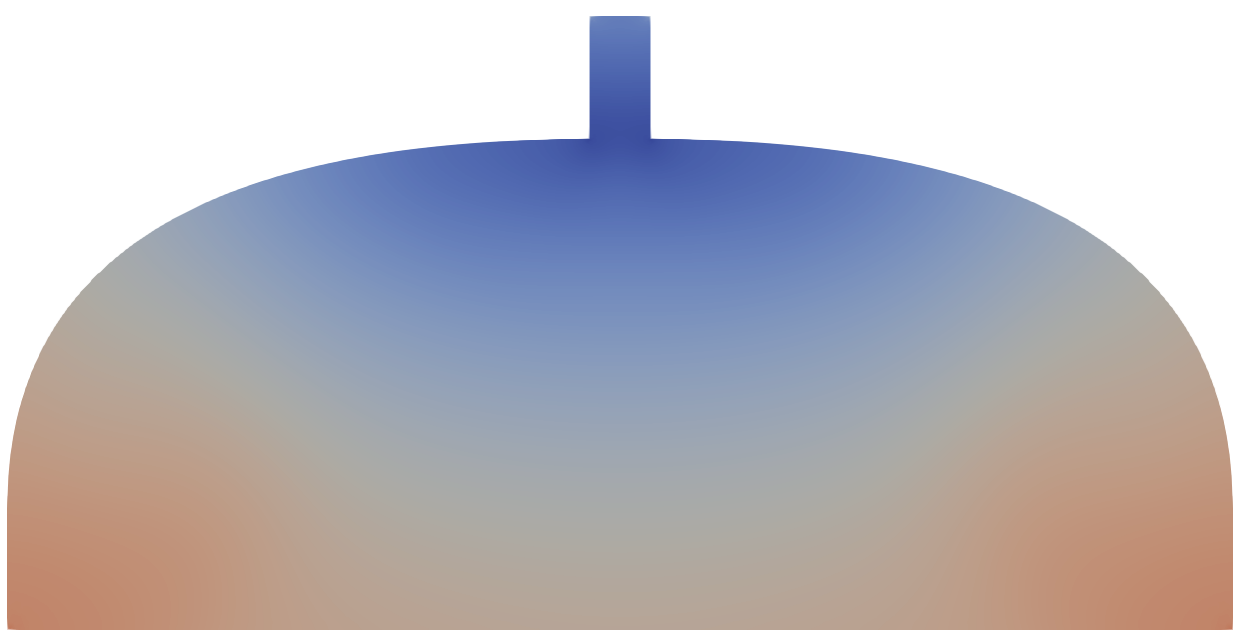
\includegraphics[width=0.96\textwidth]{pressure_field_case_0_arch_07_20.png}
        \subcaption{}
    \end{subfigure}
    \begin{subfigure}[b]{0.30\textwidth}
        \centering
        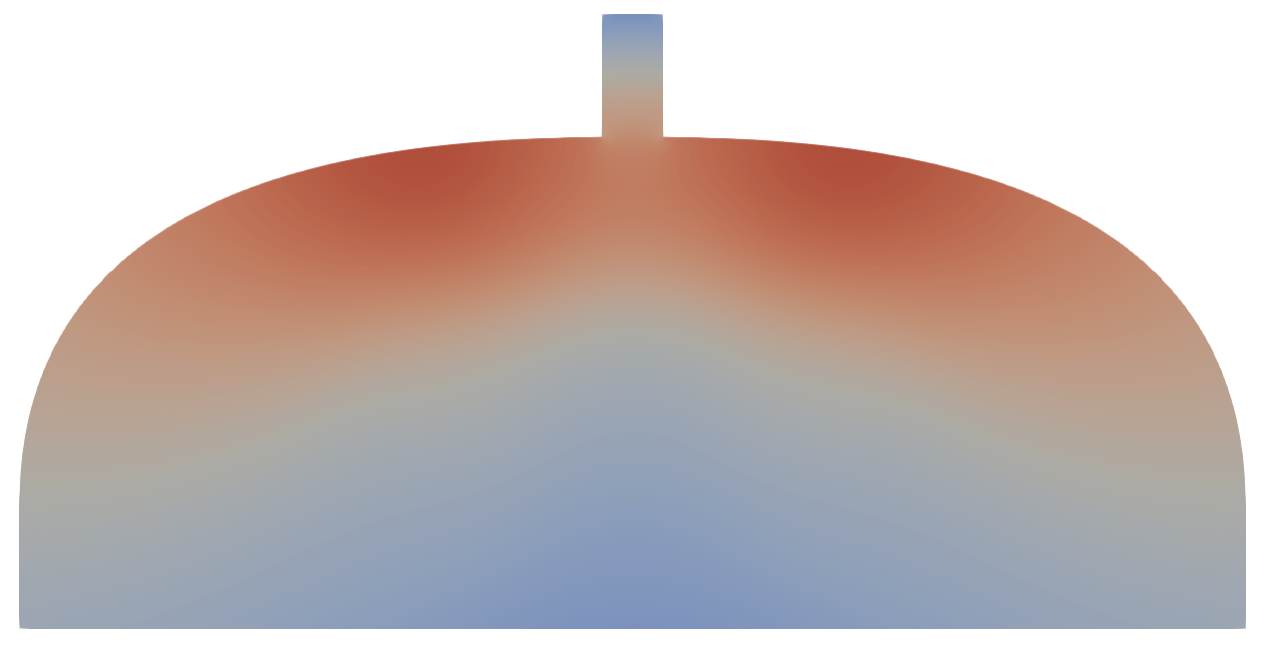
\includegraphics[width=0.96\textwidth]{pressure_field_case_0_arch_11_20.png}
        \subcaption{}
    \end{subfigure}
    \begin{subfigure}[b]{0.30\textwidth}
        \centering
        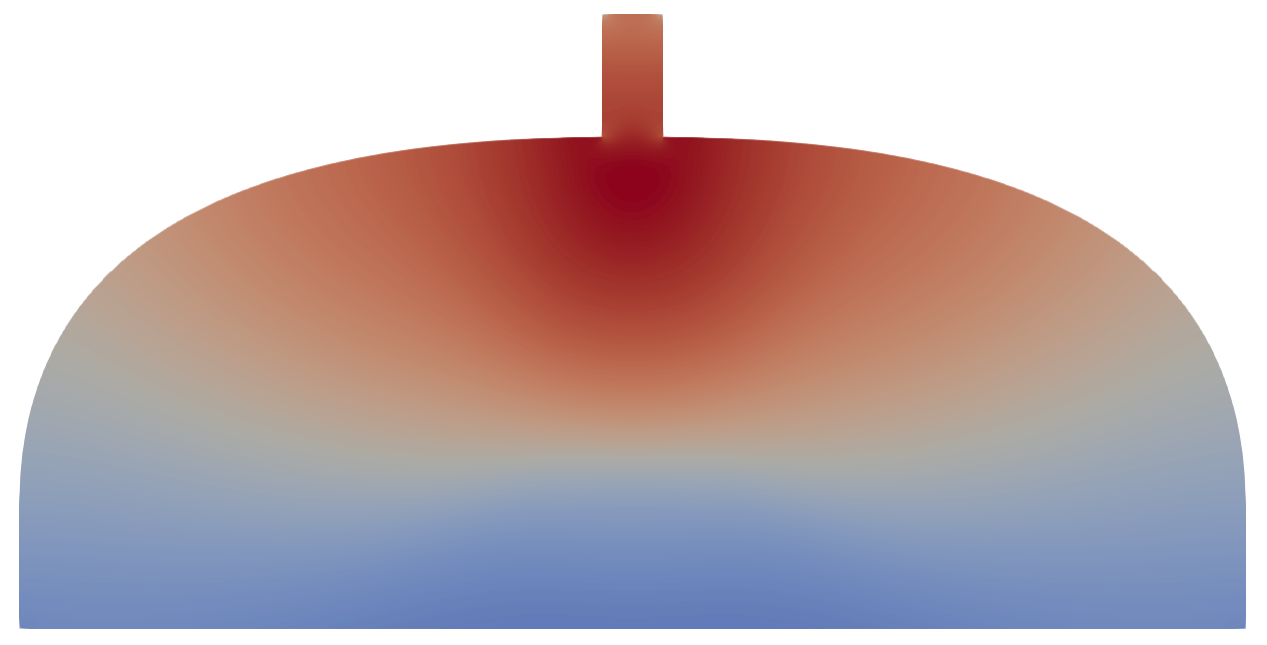
\includegraphics[width=0.96\textwidth]{pressure_field_case_0_arch_14_20.png}
        \subcaption{}
    \end{subfigure}
    \begin{subfigure}[b]{0.08\textwidth}
        \centering
        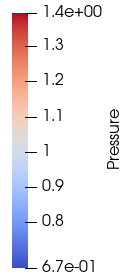
\includegraphics[width=0.96\textwidth]{pressure_field_case_0_arch_axis.png}
        \subcaption{}
    \end{subfigure}
    \captionsetup{font=scriptsize}
    \caption{
    Pressure contours at 3 time points (a:$\frac{7}{20}T$,b:$\frac{11}{20}T$,c:$\frac{14}{20}T$) during the ``upward push half-cycle'' for the arched chamber under Case 0.
    Maximum pressure occurs at the moment of emission (c);
    the smooth design of the lower part of the arched chamber does not alleviate maximum pressure;
    the flat upper part of the chamber disperses pressure (b).
    }
    \label{fig:pressure_field_case_0_arch}
\end{figure}

\begin{figure}[htbp]
    %\centering
    \begin{subfigure}[b]{0.44\textwidth}
        \centering
        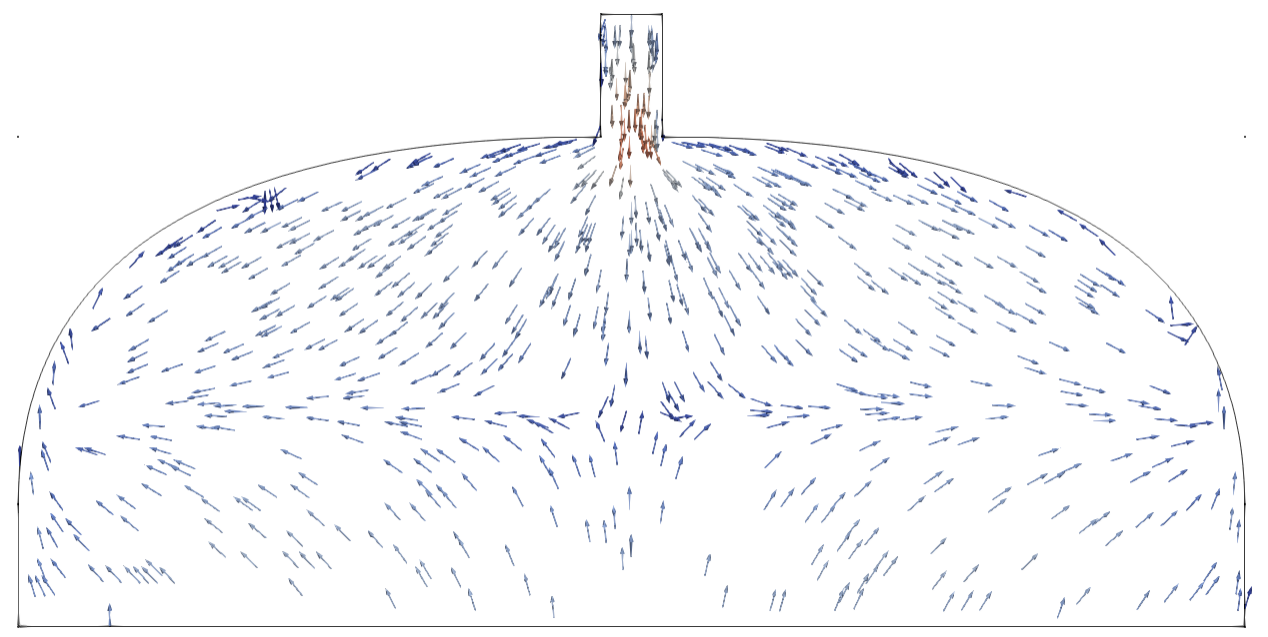
\includegraphics[width=0.96\textwidth]{velocity_field_case_0_arch_04_20.png}
        \subcaption{}
    \end{subfigure}
    \begin{subfigure}[b]{0.44\textwidth}
        \centering
        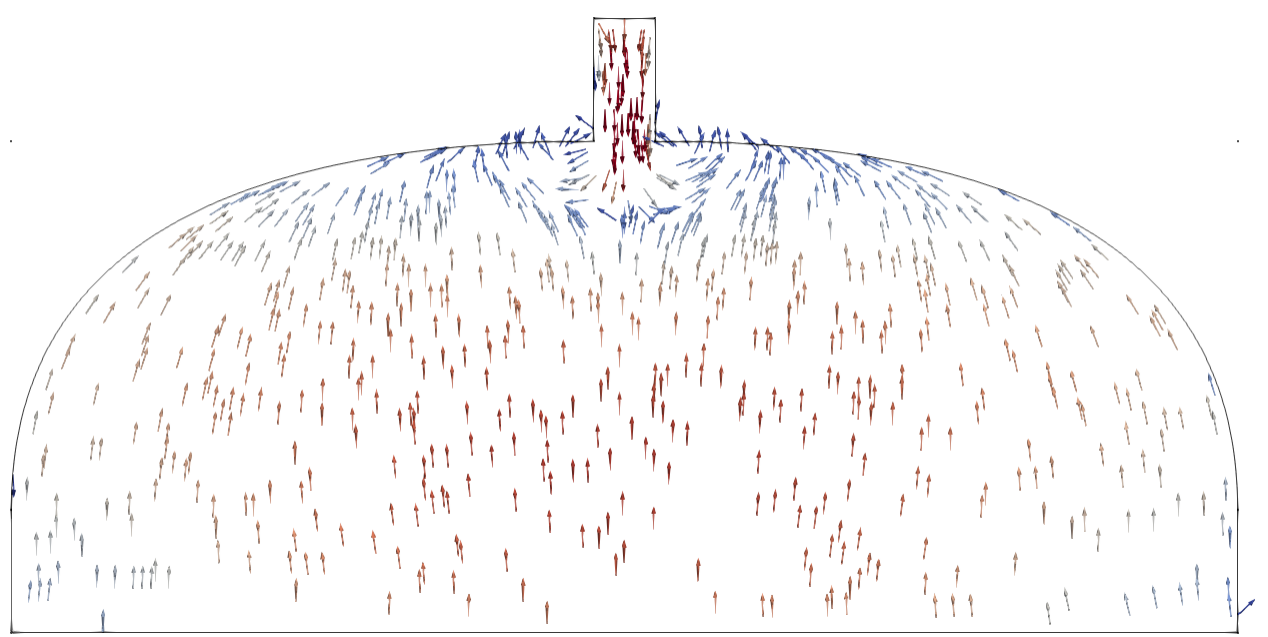
\includegraphics[width=0.96\textwidth]{velocity_field_case_0_arch_07_20.png}
        \subcaption{}
    \end{subfigure}
    \begin{subfigure}[b]{0.10\textwidth}
        \centering
        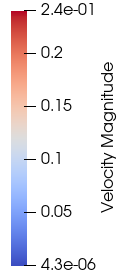
\includegraphics[width=0.96\textwidth]{velocity_field_case_0_arch_axis.png}
        \vspace{1.0pt}
    \end{subfigure}
    \\
    \begin{subfigure}[b]{0.44\textwidth}
        \centering
        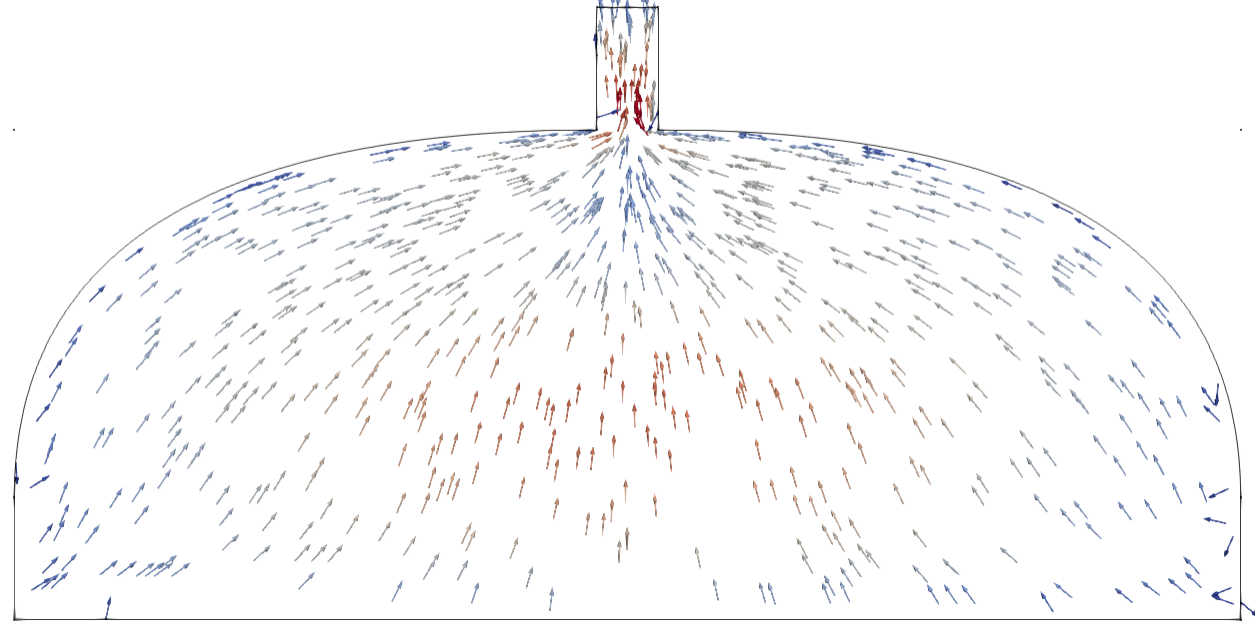
\includegraphics[width=0.96\textwidth]{velocity_field_case_0_arch_12_20.png}
        \subcaption{}
    \end{subfigure}
    \begin{subfigure}[b]{0.44\textwidth}
        \centering
        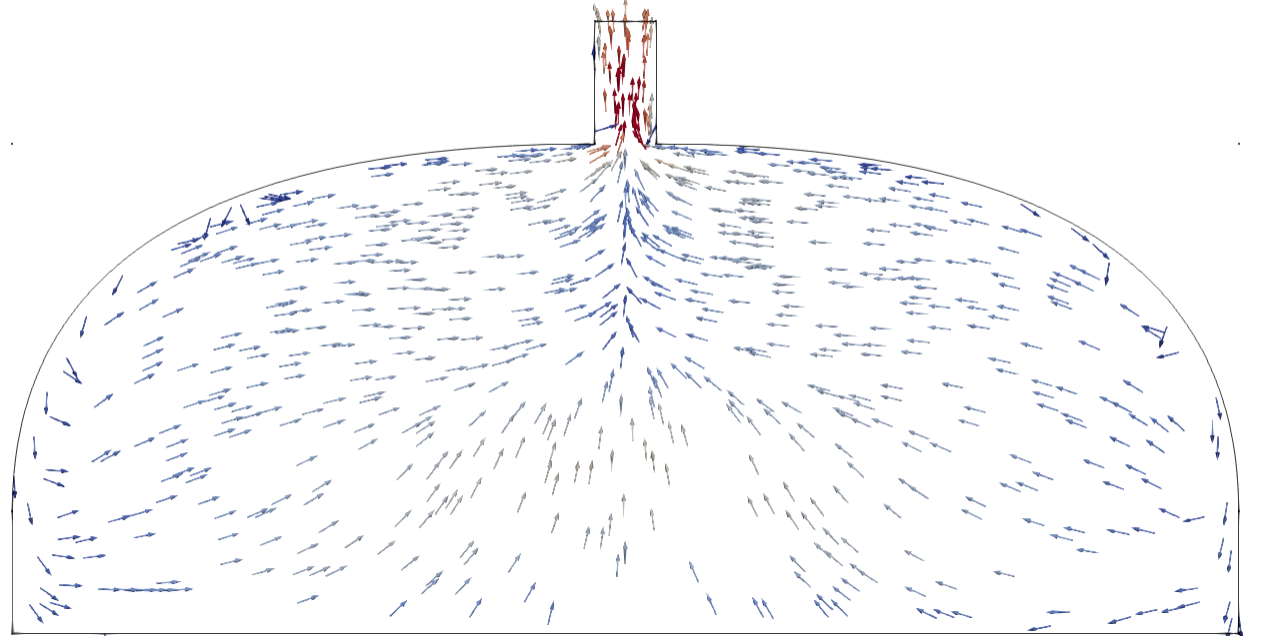
\includegraphics[width=0.96\textwidth]{velocity_field_case_0_arch_13_20.png}
        \subcaption{}
    \end{subfigure}
    \captionsetup{font=scriptsize}
    \caption{
    Velocity vector diagrams at 4 time points (a:$\frac{4}{20}T$,b:$\frac{7}{20}T$,c:$\frac{12}{20}T$,d:$\frac{13}{20}T$) during the ``upward push half-cycle'' for the arched chamber under Case 0.
    The upper limit of the color bar is not the maximum velocity value.
    During the emission phase, the left and right portions of the fluid undergo a ``head-on collision'' (c).
    }
    \label{fig:velocity_field_case_0_arch}
\end{figure}

Summary for the arched chamber shape regarding wall pressure and exit velocity performance:
1.The upward convex design helps reduce the pressure on the chamber walls when fluid first enters (Figure \ref{fig:pressure_field_case_0_arch}(a)),
but the maximum pressure occurs at the emission moment (Figure \ref{fig:pressure_field_case_0_arch}(c)).

During the emission phase, the fluid in the left and right halves of the chamber undergoes a ``head-on collision'' (Figure \ref{fig:velocity_field_case_0_arch}(c)(d)),
which likely causes significant loss of fluid kinetic energy.

These are not unique characteristics of this specific arched shape; all upward convex chambers share similar properties.

As a critical shape of the upward convex type, pressure contours for the ``Inverted V-shape'' are shown in Figure \ref{fig:pressure_field_case_0_inverted_v}, and velocity vectors in Figure \ref{fig:velocity_field_case_0_inverted_v}.
Similarly, the focus is on the upward push half-cycle.

\begin{figure}[htbp]
    \centering
    \begin{subfigure}[b]{0.30\textwidth}
        \centering
        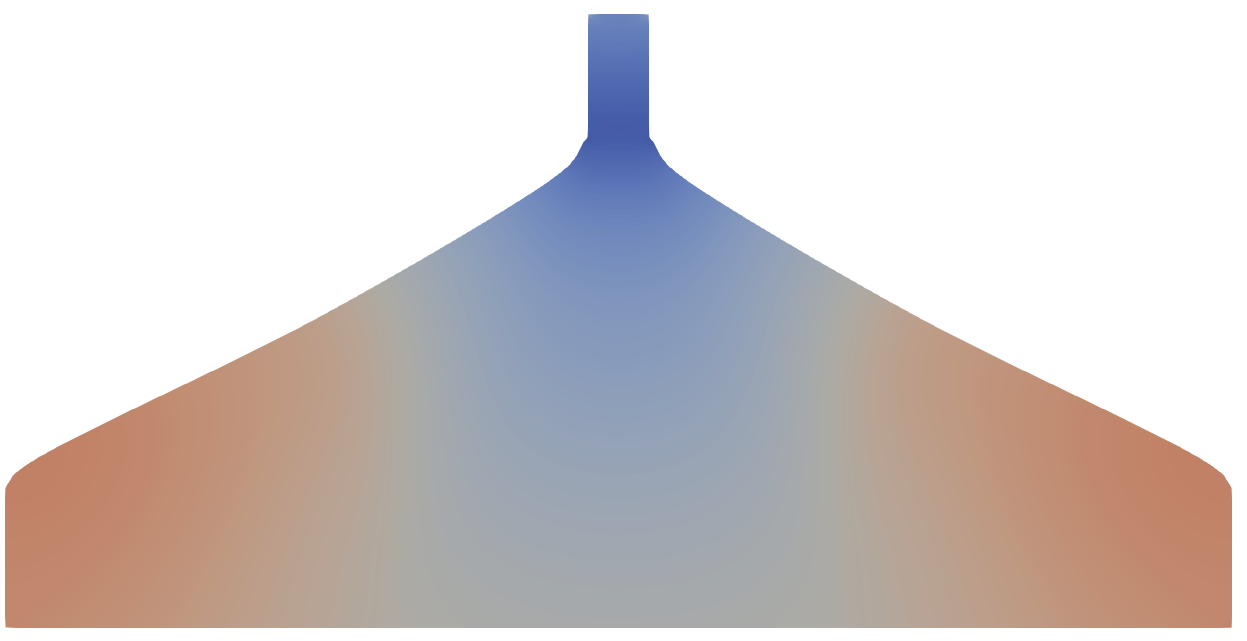
\includegraphics[width=0.96\textwidth]{pressure_field_case_0_inverted_v_07_20.png}
        \subcaption{}
    \end{subfigure}
    \begin{subfigure}[b]{0.30\textwidth}
        \centering
        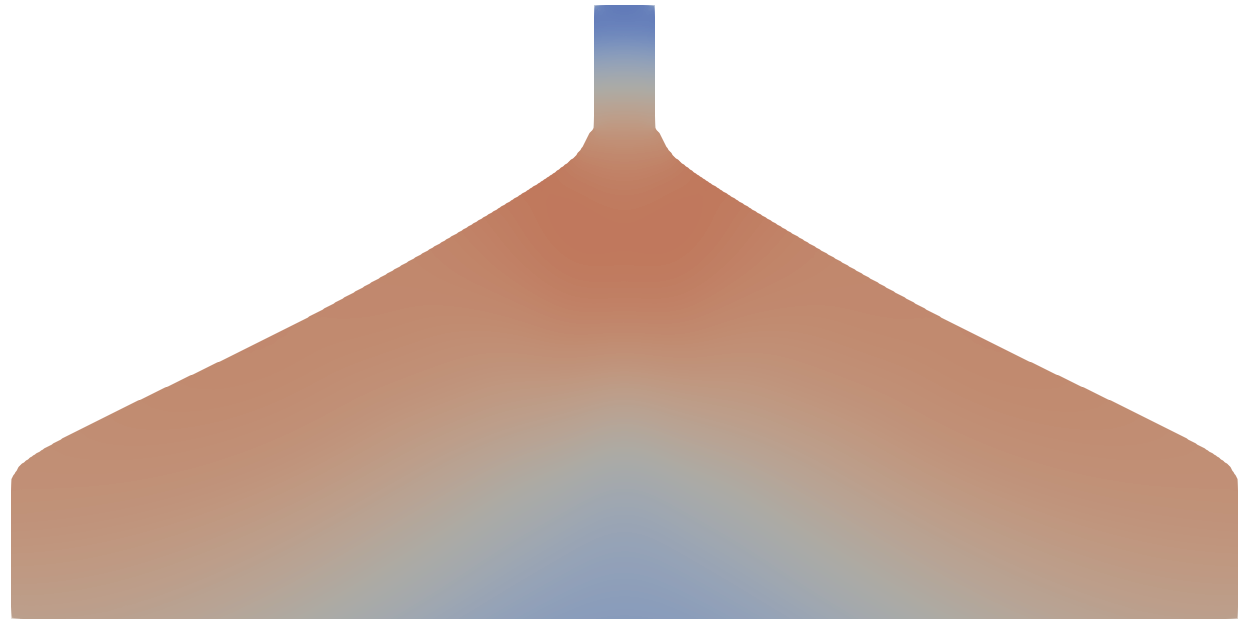
\includegraphics[width=0.96\textwidth]{pressure_field_case_0_inverted_v_10_20.png}
        \subcaption{}
    \end{subfigure}
    \begin{subfigure}[b]{0.30\textwidth}
        \centering
        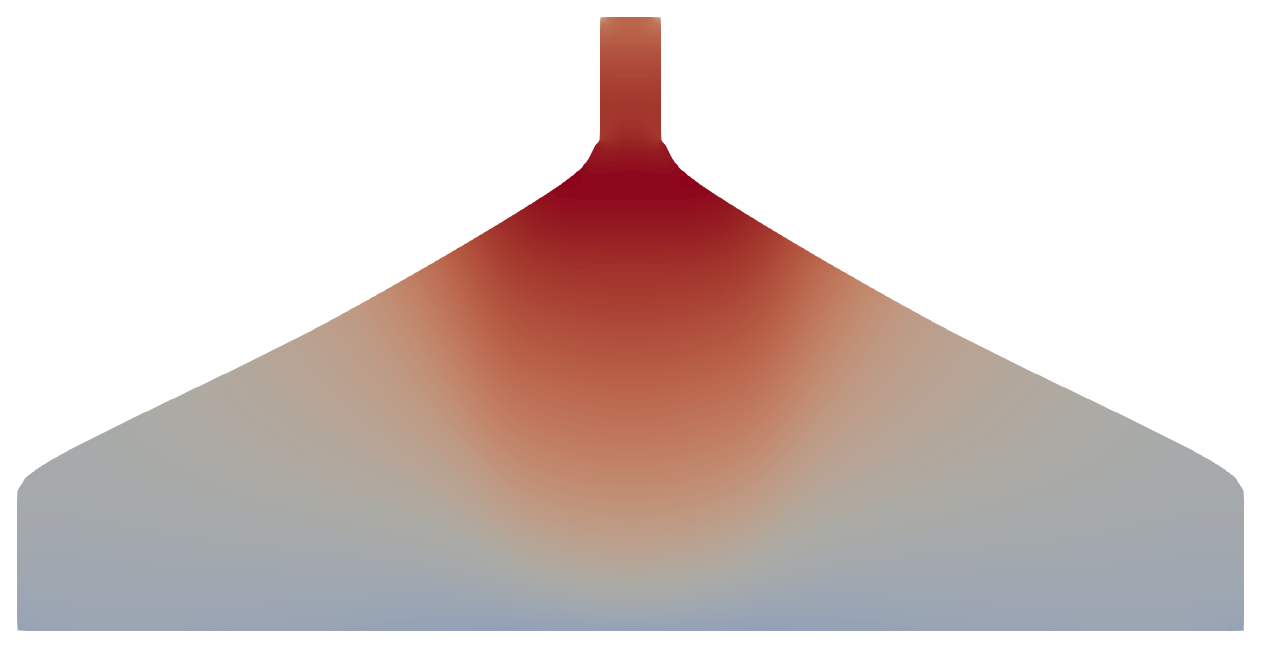
\includegraphics[width=0.96\textwidth]{pressure_field_case_0_inverted_v_13_20.png}
        \subcaption{}
    \end{subfigure}
    \begin{subfigure}[b]{0.08\textwidth}
        \centering
        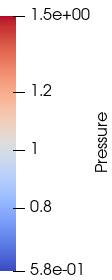
\includegraphics[width=0.96\textwidth]{pressure_field_case_0_inverted_v_axis.png}
        \subcaption{}
    \end{subfigure}
    \captionsetup{font=scriptsize}
    \caption{
    Pressure contours at 3 time points (a:$\frac{7}{20}T$,b:$\frac{10}{20}T$,c:$\frac{13}{20}T$) during the ``upward push half-cycle'' for the ``inverted V-shape'' chamber under Case 0.
    Compared to the arched shape, it lacks the pressure dispersion effect of a flat upper section (b).
    }
    \label{fig:pressure_field_case_0_inverted_v}
\end{figure}

\begin{figure}[htbp]
    %\centering
    \begin{subfigure}[b]{0.44\textwidth}
        \centering
        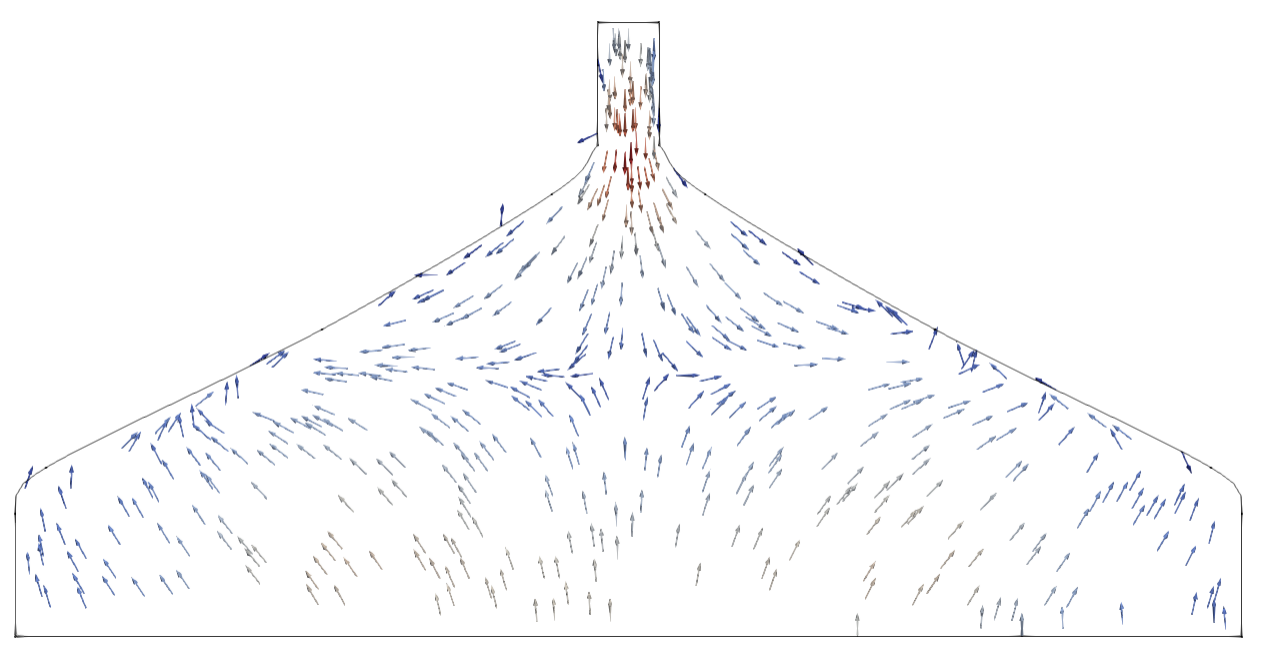
\includegraphics[width=0.96\textwidth]{velocity_field_case_0_inverted_v_04_20.png}
        \subcaption{}
    \end{subfigure}
    \begin{subfigure}[b]{0.44\textwidth}
        \centering
        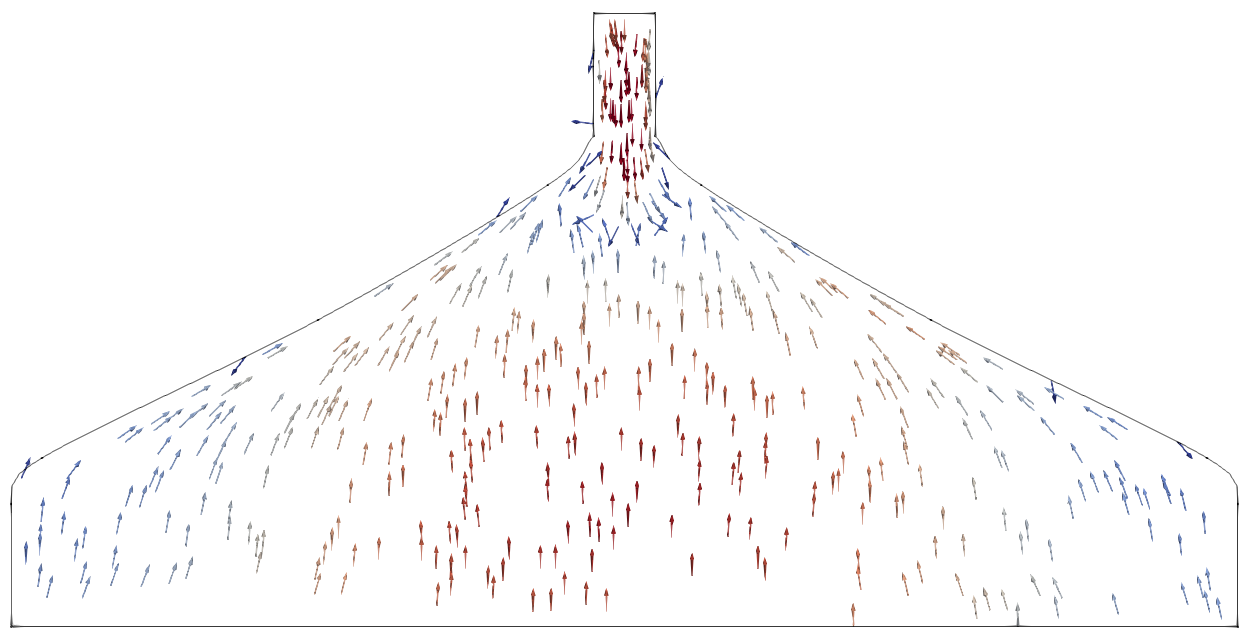
\includegraphics[width=0.96\textwidth]{velocity_field_case_0_inverted_v_07_20.png}
        \subcaption{}
    \end{subfigure}
    \begin{subfigure}[b]{0.10\textwidth}
        \centering
        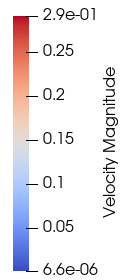
\includegraphics[width=0.96\textwidth]{velocity_field_case_0_inverted_v_axis.png}
        \vspace{1.0pt}
    \end{subfigure}
    \\
    \begin{subfigure}[b]{0.44\textwidth}
        \centering
        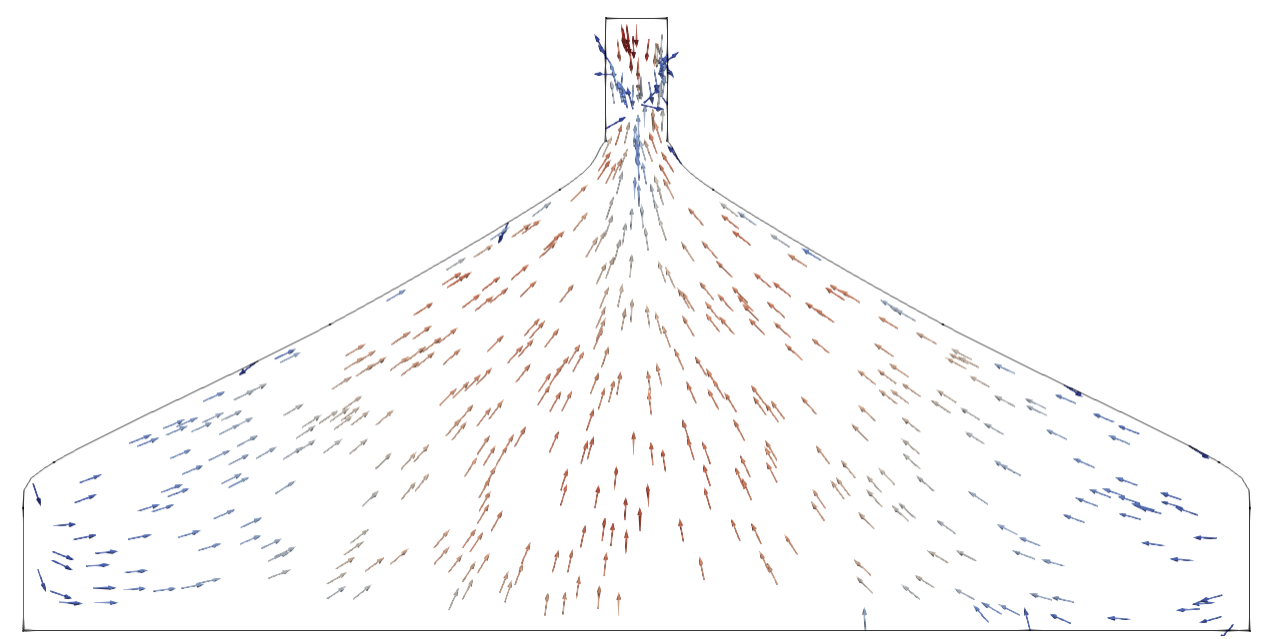
\includegraphics[width=0.96\textwidth]{velocity_field_case_0_inverted_v_10_20.png}
        \subcaption{}
    \end{subfigure}
    \begin{subfigure}[b]{0.44\textwidth}
        \centering
        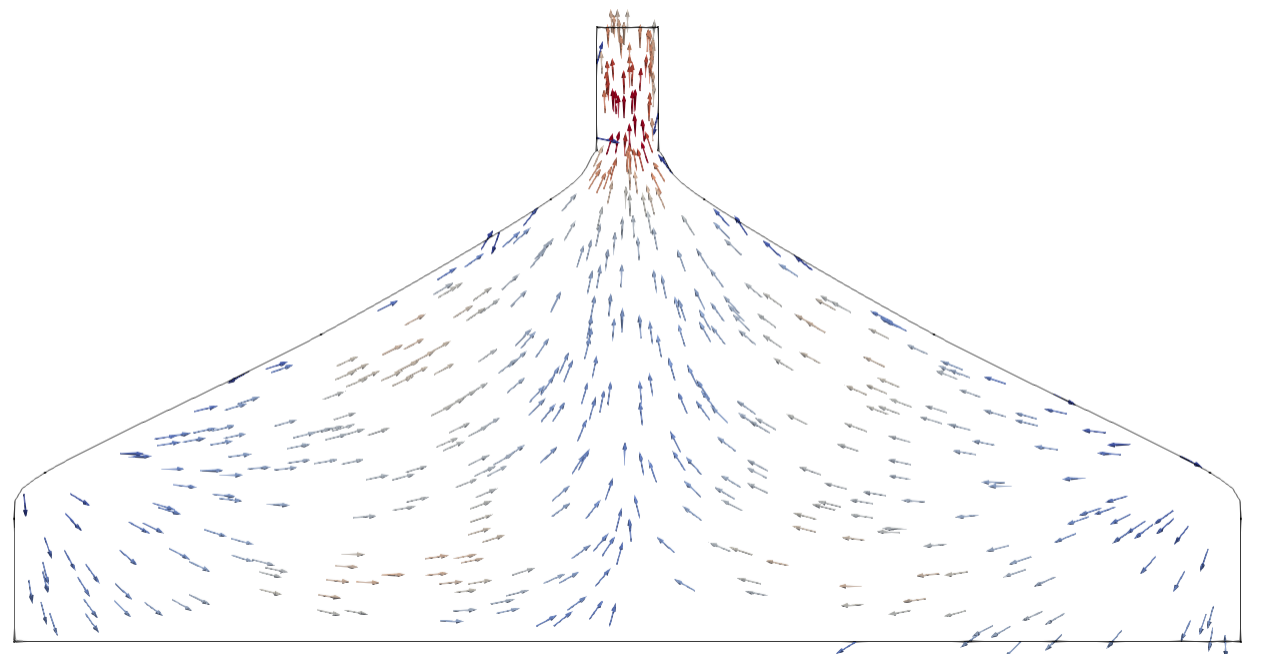
\includegraphics[width=0.96\textwidth]{velocity_field_case_0_inverted_v_12_20.png}
        \subcaption{}
    \end{subfigure}
    \captionsetup{font=scriptsize}
    \caption{
    Velocity vector diagrams at 4 time points (a:$\frac{4}{20}T$,b:$\frac{7}{20}T$,c:$\frac{10}{20}T$,d:$\frac{12}{20}T$) during the ``upward push half-cycle'' for the ``inverted V-shape'' chamber under Case 0.
    Compared to the arched shape, it significantly mitigates the collision of fluids during the emission phase (c)(d).
    }
    \label{fig:velocity_field_case_0_inverted_v}
\end{figure}

Regarding the wall pressure and outlet velocity performance, here is a simple summary of the ``inverted V-shaped'' chamber:
The ``inverted V-shaped'' chamber design reduces the smoothness of the lower portion of the chamber, appropriately increasing the pressure when the incoming flow of a new cycle contacts the lower chamber walls (Figure \ref{fig:pressure_field_case_0_inverted_v}(a)),
the maximum pressure still occurs at the moment of ejection (Figure \ref{fig:pressure_field_case_0_inverted_v}(c)).
However, the absence of the pressure-dispersing effect found in the upper part of arched chambers (Figure \ref{fig:pressure_field_case_0_inverted_v}(b)) leads to an increase in maximum pressure compared to the arched design.
Compared to the arched chamber, the ``inverted V-shaped'' chamber design reduces fluid collisions within the chamber (especially during the ejection phase (\ref{fig:velocity_field_case_0_inverted_v}(c)(d))).

The performance of other convex chamber shapes is roughly between the arched chamber shape and the ``inverted V-shaped'' chamber shape.

Based on the analysis of arched and ``inverted V-shaped'' chamber shapes, researchers found that during the ejection phase, the pressure reaches its maximum value, and the fluid undergoes violent mutual collisions, dissipating kinetic energy.
Or rather, there is still room for further improvement in the pressure during the process when the incoming flow of a new cycle just contacts the lower wall of the chamber;
there is still room for optimization in the flow during the ejection phase.

\subsection{Characteristics of the Internal Flow Field of ``Inverted T-shaped'' and ``S-shaped'' Chamber Shapes}\indent

The pressure cloud map under the ``inverted T-shaped'' chamber shape is shown in Figure \ref{fig:pressure_field_case_0_inverted_t}, and the velocity vector diagram is shown in Figure \ref{fig:velocity_field_case_0_inverted_t}.

\begin{figure}[htbp]
    \centering
    \begin{subfigure}[b]{0.30\textwidth}
        \centering
        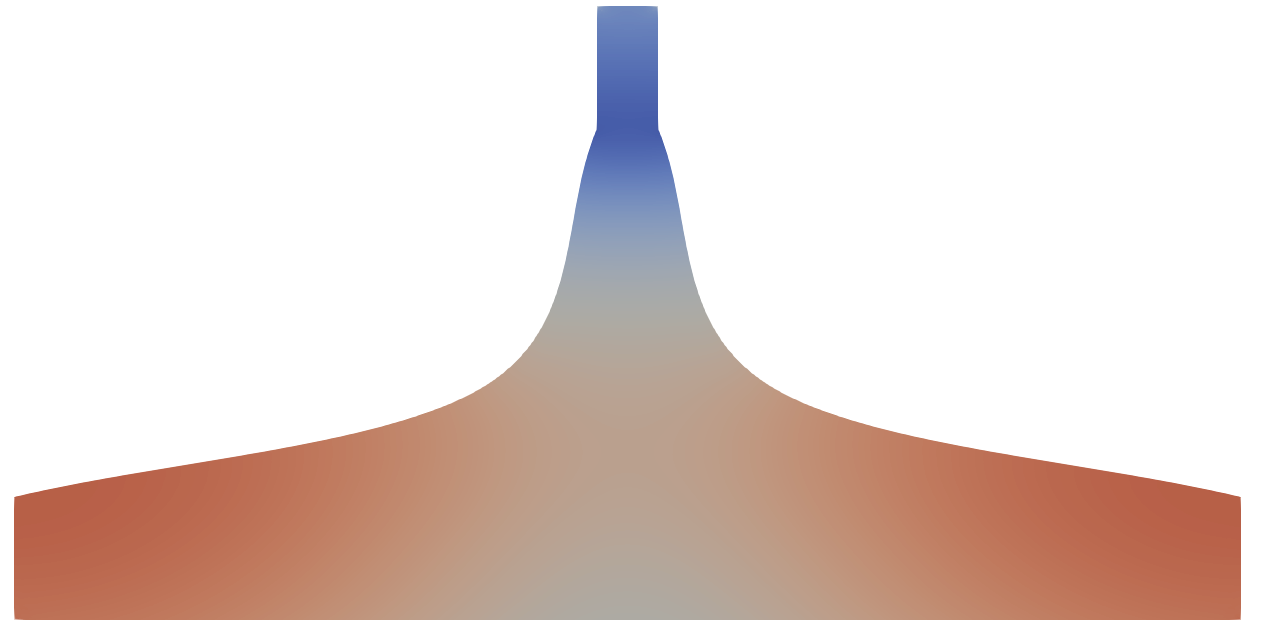
\includegraphics[width=0.96\textwidth]{pressure_field_case_0_inverted_t_07_20.png}
        \subcaption{}
    \end{subfigure}
    \begin{subfigure}[b]{0.30\textwidth}
        \centering
        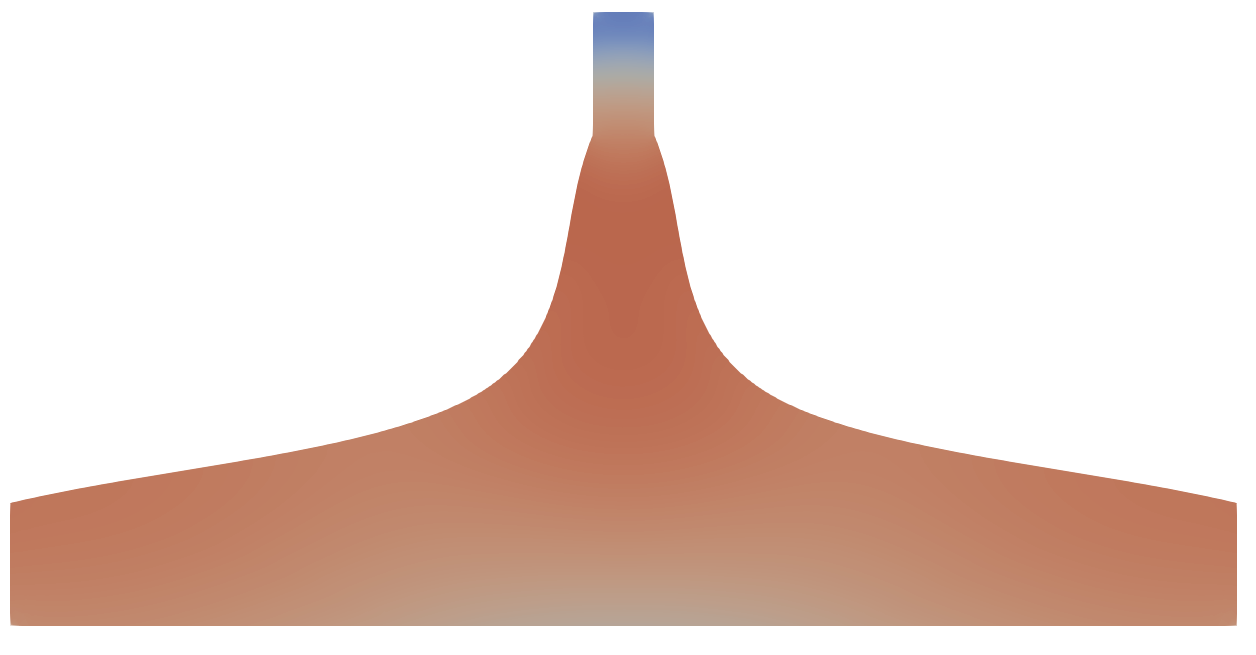
\includegraphics[width=0.96\textwidth]{pressure_field_case_0_inverted_t_10_20.png}
        \subcaption{}
    \end{subfigure}
    \begin{subfigure}[b]{0.30\textwidth}
        \centering
        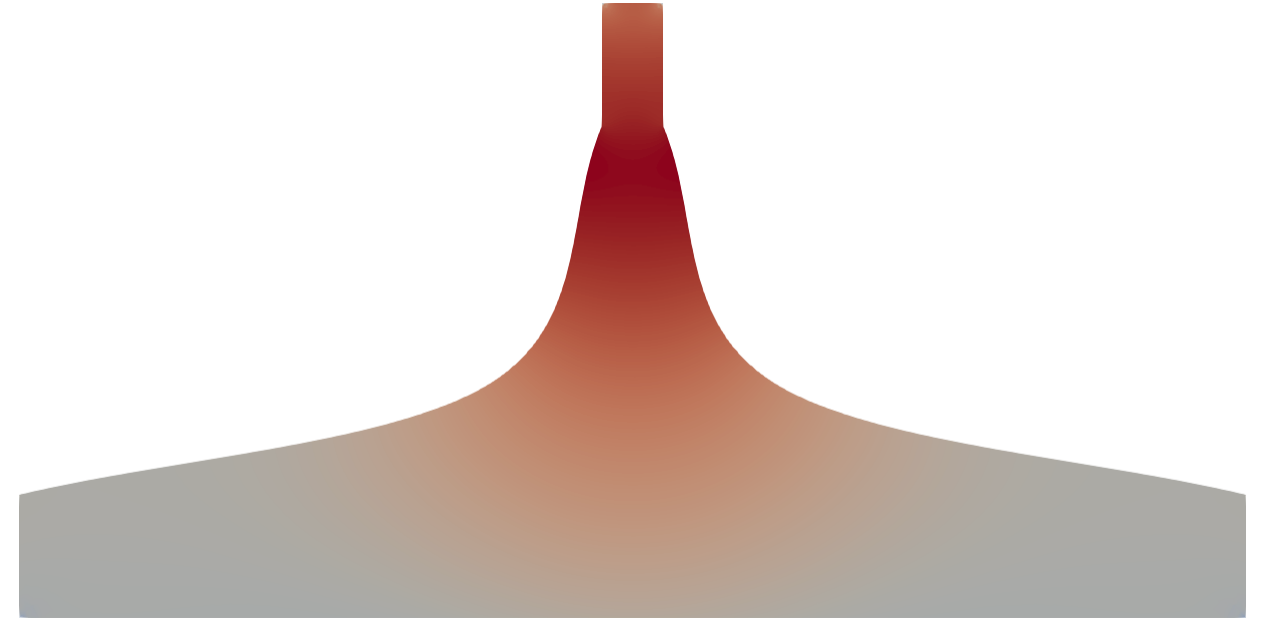
\includegraphics[width=0.96\textwidth]{pressure_field_case_0_inverted_t_13_20.png}
        \subcaption{}
    \end{subfigure}
    \begin{subfigure}[b]{0.08\textwidth}
        \centering
        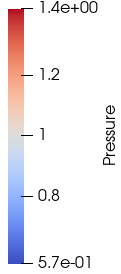
\includegraphics[width=0.96\textwidth]{pressure_field_case_0_inverted_t_axis.png}
        \subcaption{}
    \end{subfigure}
    \captionsetup{font=scriptsize}
    \caption{
    Pressure contours at 3 time points (a:$\frac{7}{20}T$,b:$\frac{10}{20}T$,c:$\frac{13}{20}T$) during the ``upward push half-cycle'' for the ``inverted T-shape'' chamber under Case 0.
    Although the bottom will bear greater pressure (a), the maximum pressure appears at the ejection moment (c).
    }
    \label{fig:pressure_field_case_0_inverted_t}
\end{figure}

\begin{figure}[htbp]
    %\centering
    \begin{subfigure}[b]{0.44\textwidth}
        \centering
        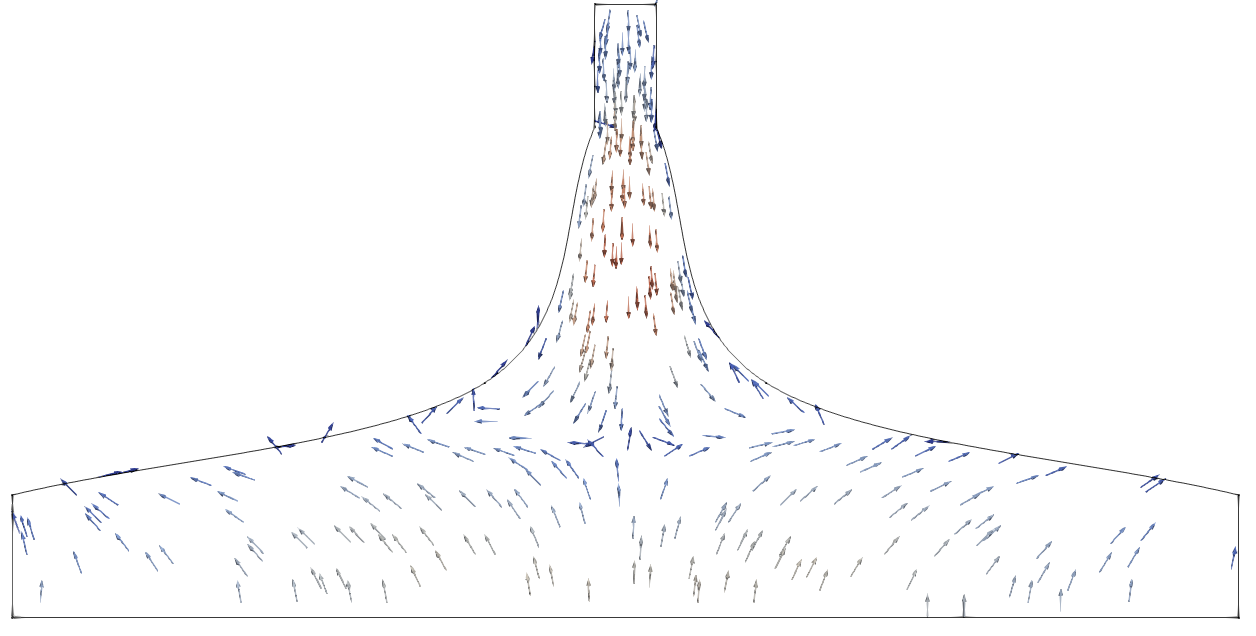
\includegraphics[width=0.96\textwidth]{velocity_field_case_0_inverted_t_03_20.png}
        \subcaption{}
    \end{subfigure}
    \begin{subfigure}[b]{0.44\textwidth}
        \centering
        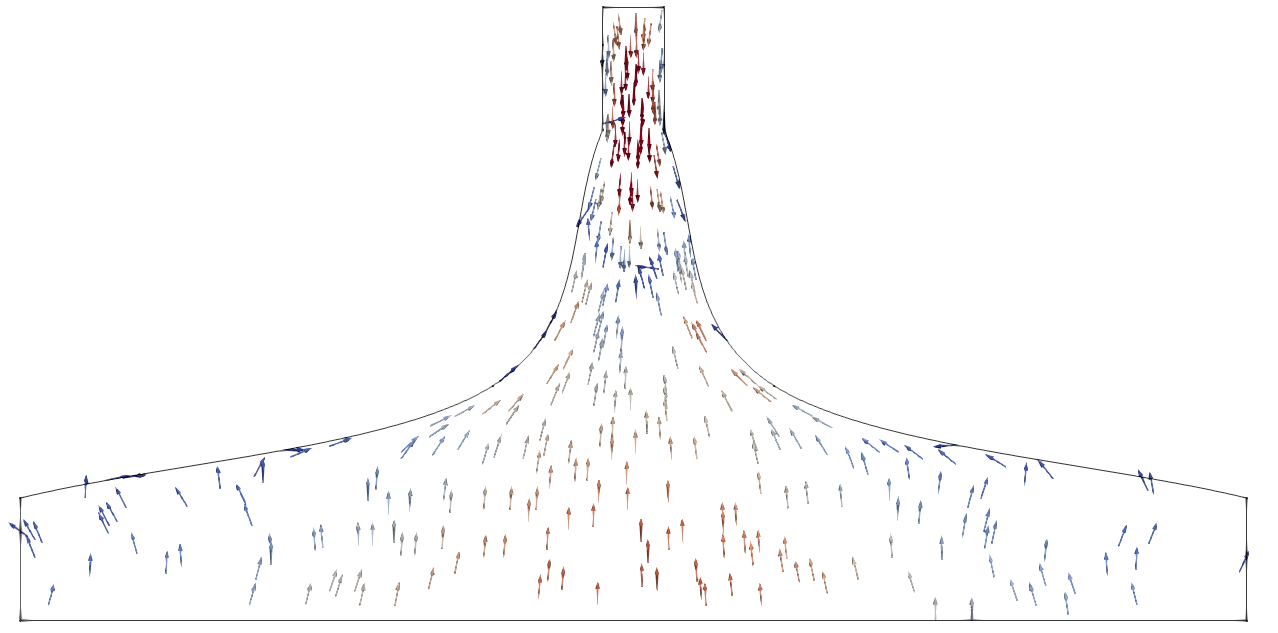
\includegraphics[width=0.96\textwidth]{velocity_field_case_0_inverted_t_06_20.png}
        \subcaption{}
    \end{subfigure}
    \begin{subfigure}[b]{0.10\textwidth}
        \centering
        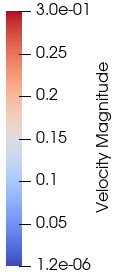
\includegraphics[width=0.96\textwidth]{velocity_field_case_0_inverted_t_axis.png}
        \vspace{1.0pt}
    \end{subfigure}
    \\
    \begin{subfigure}[b]{0.44\textwidth}
        \centering
        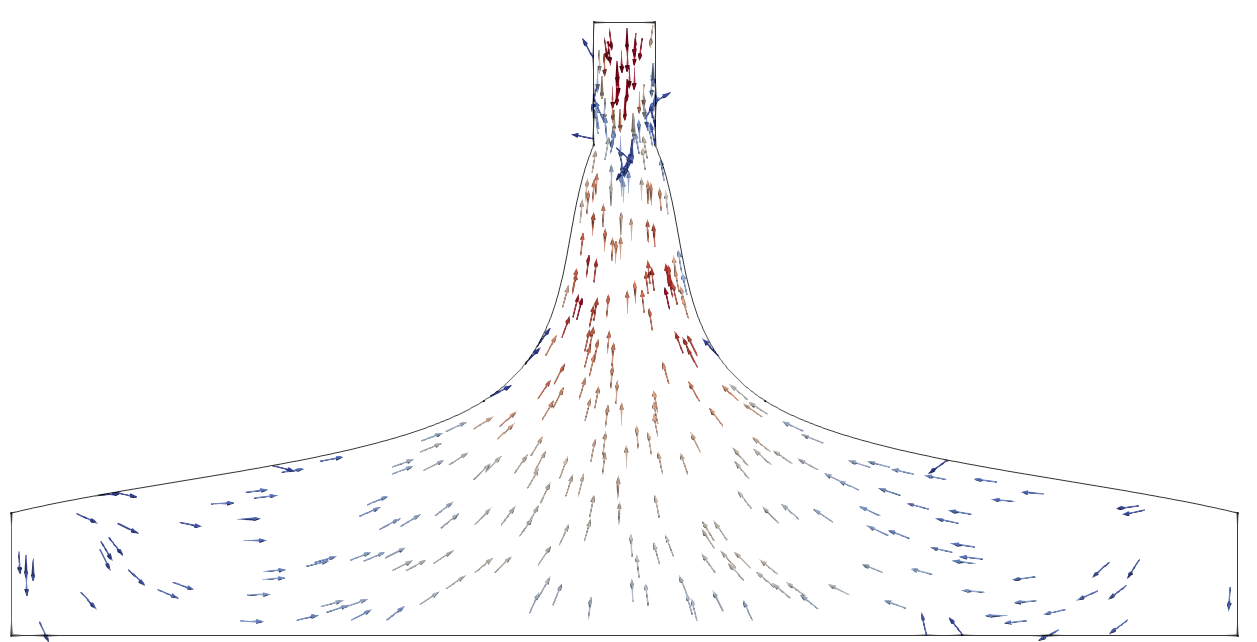
\includegraphics[width=0.96\textwidth]{velocity_field_case_0_inverted_t_09_20.png}
        \subcaption{}
    \end{subfigure}
    \begin{subfigure}[b]{0.44\textwidth}
        \centering
        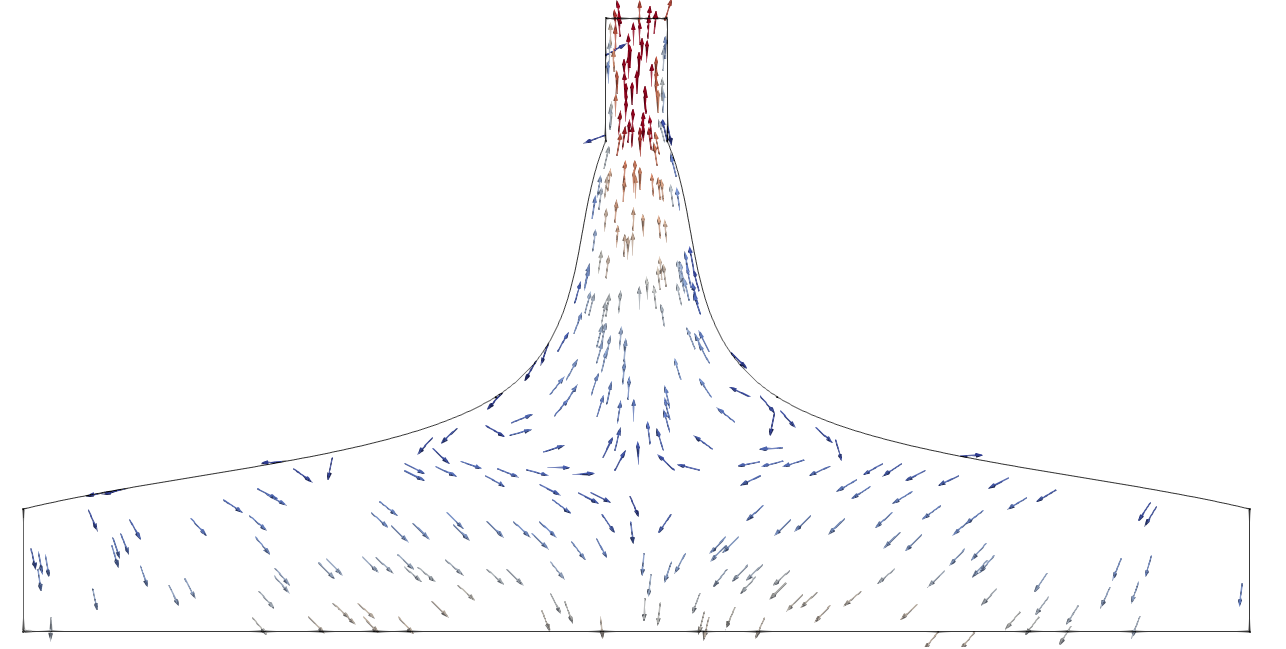
\includegraphics[width=0.96\textwidth]{velocity_field_case_0_inverted_t_13_20.png}
        \subcaption{}
    \end{subfigure}
    \captionsetup{font=scriptsize}
    \caption{
    Velocity vector diagrams at 4 time points (a:$\frac{3}{20}T$,b:$\frac{6}{20}T$,c:$\frac{9}{20}T$,d:$\frac{13}{20}T$) during the ``upward push half-cycle'' for the ``inverted T-shape'' chamber under Case 0.
    Although more fluid collisions occur at the bottom, fluid collisions in the ejection phase are significantly reduced (c)(d).
    }
    \label{fig:velocity_field_case_0_inverted_t}
\end{figure}

Summarizing the ``inverted T-shaped'' chamber shape regarding wall pressure and outlet velocity performance:
1. The ``inverted T-shaped'' chamber shape more fully utilizes the pressure-bearing capacity of the lower part of the chamber (Figure \ref{fig:pressure_field_case_0_inverted_t}(a));
it still lacks the pressure dispersion effect of the upper part of the arched chamber (Figure \ref{fig:pressure_field_case_0_inverted_t}(b)), and the maximum pressure is increased relative to the arched shape (Figure \ref{fig:pressure_field_case_0_inverted_t}(c));
2. Compared to the ``inverted V-shaped'' chamber, mutual collisions of fluid within the chamber and collisions between fluid and collisions with the chamber mainly occur in the lower part of the chamber (and the fluid velocity in this part is lower), while during the ejection phase,
mutual collisions of the fluid are minimal (Figure \ref{fig:velocity_field_case_0_inverted_t}(c)(d)).

Ultimately, the ``inverted T-shaped'' achieves wall pressure and outlet velocity performance similar to the ``inverted V-shaped''.
The pressure cloud map under the ``S-shaped'' chamber shape is shown in Figure \ref{fig:pressure_field_case_0_s}, and the velocity vector diagram is shown in Figure \ref{fig:velocity_field_case_0_s}.

\begin{figure}[htbp]
    \centering
    \begin{subfigure}[b]{0.30\textwidth}
        \centering
        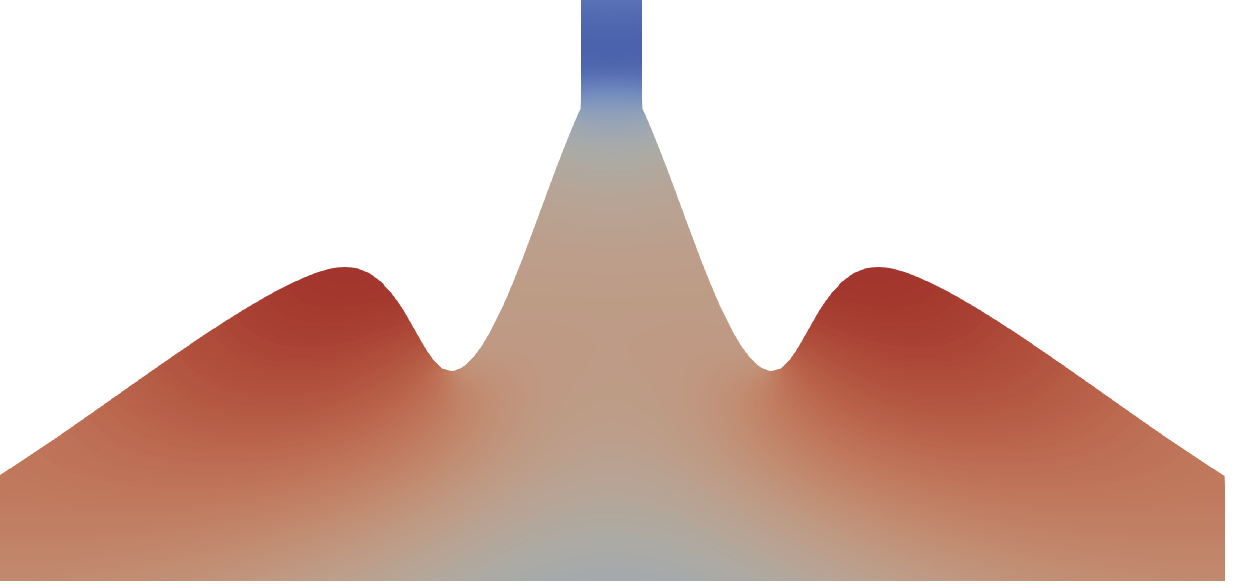
\includegraphics[width=0.96\textwidth]{pressure_field_case_0_s_09_20.png}
        \subcaption{}
    \end{subfigure}
    \begin{subfigure}[b]{0.30\textwidth}
        \centering
        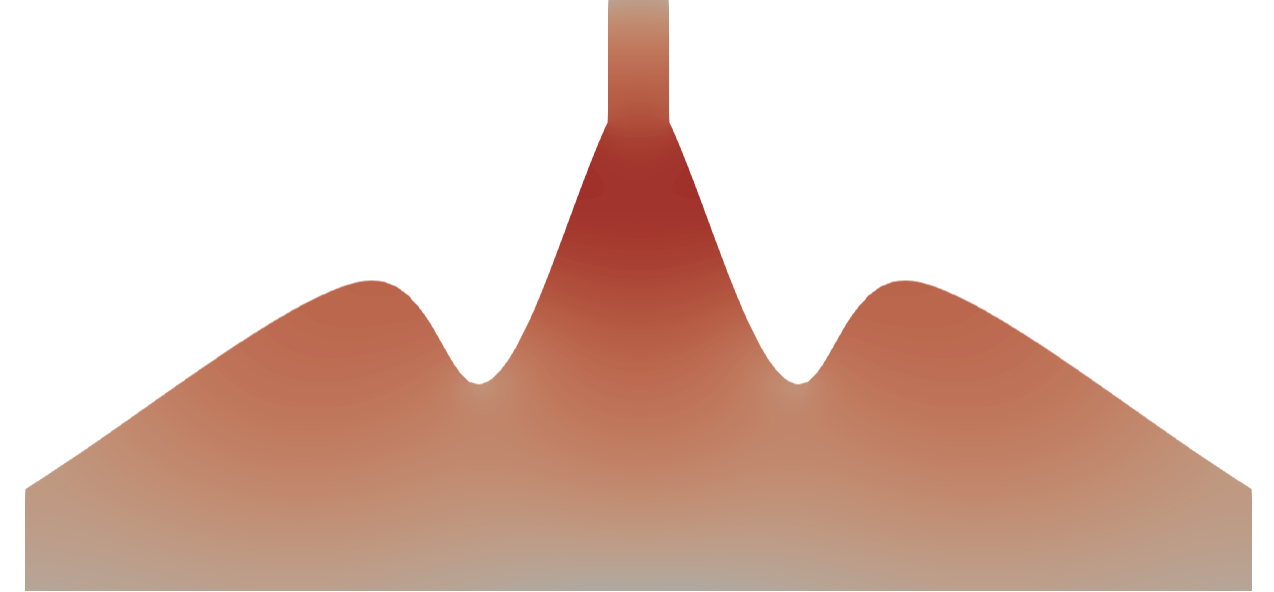
\includegraphics[width=0.96\textwidth]{pressure_field_case_0_s_12_20.png}
        \subcaption{}
    \end{subfigure}
    \begin{subfigure}[b]{0.30\textwidth}
        \centering
        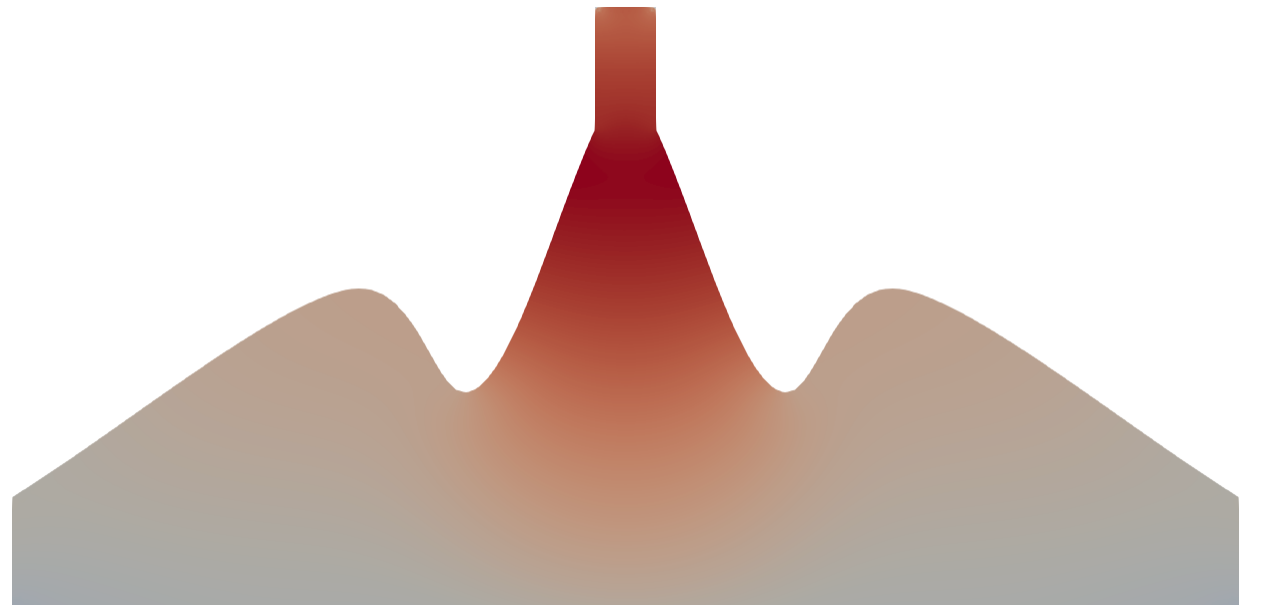
\includegraphics[width=0.96\textwidth]{pressure_field_case_0_s_14_20.png}
        \subcaption{}
    \end{subfigure}
    \begin{subfigure}[b]{0.08\textwidth}
        \centering
        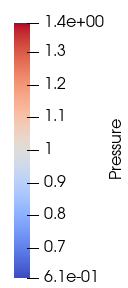
\includegraphics[width=0.96\textwidth]{pressure_field_case_0_s_axis.png}
        \subcaption{}
    \end{subfigure}
    \captionsetup{font=scriptsize}
    \caption{
    Pressure contours at 3 time points (a:$\frac{9}{20}T$,b:$\frac{12}{20}T$,c:$\frac{14}{20}T$) during the ``upward push half-cycle'' for the ``S-shape'' chamber under Case 0.
    Although the ``curved pocket'' bears greater pressure (a), the maximum pressure appears in the ejection phase (c).
    }
    \label{fig:pressure_field_case_0_s}
\end{figure}

\begin{figure}[htbp]
    %\centering
    \begin{subfigure}[b]{0.30\textwidth}
        \centering
        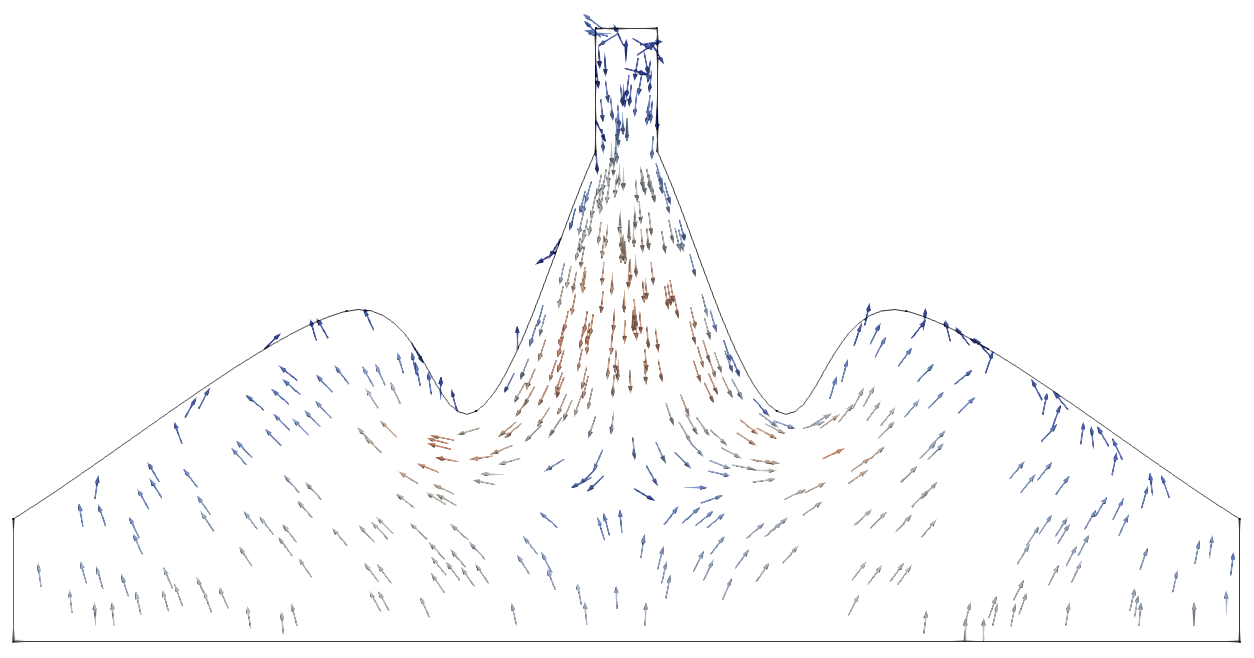
\includegraphics[width=0.96\textwidth]{velocity_field_case_0_s_03_20.png}
        \subcaption{}
    \end{subfigure}
    \begin{subfigure}[b]{0.30\textwidth}
        \centering
        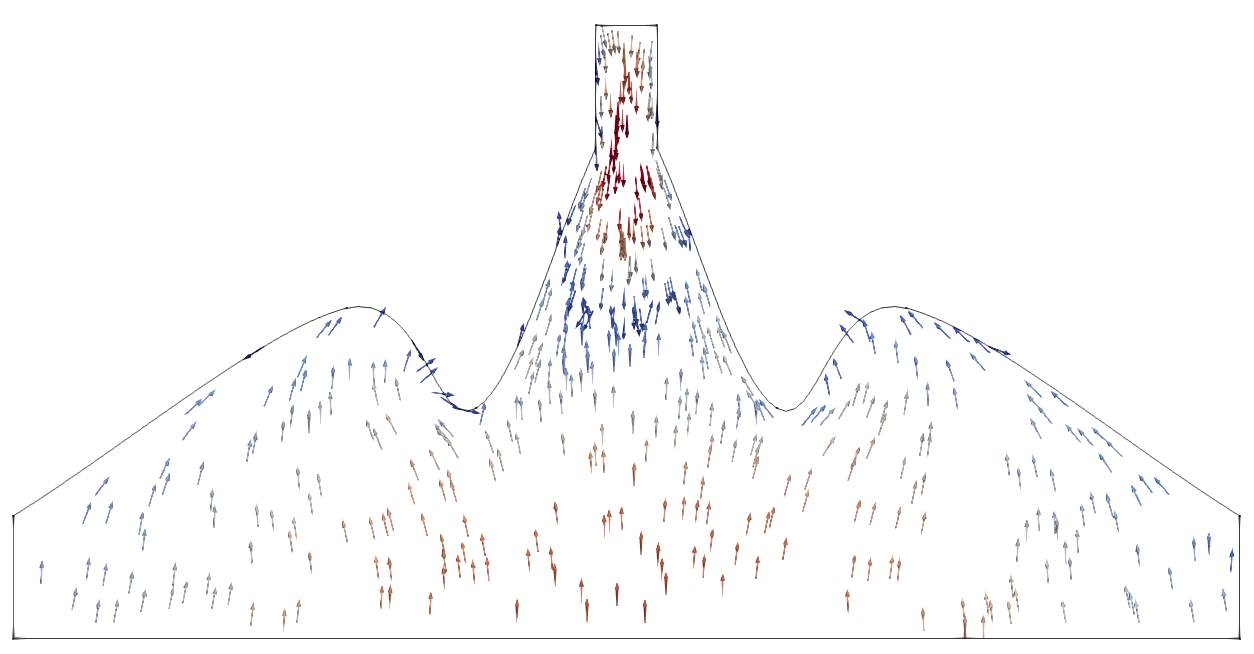
\includegraphics[width=0.96\textwidth]{velocity_field_case_0_s_06_20.png}
        \subcaption{}
    \end{subfigure}
    \begin{subfigure}[b]{0.30\textwidth}
        \centering
        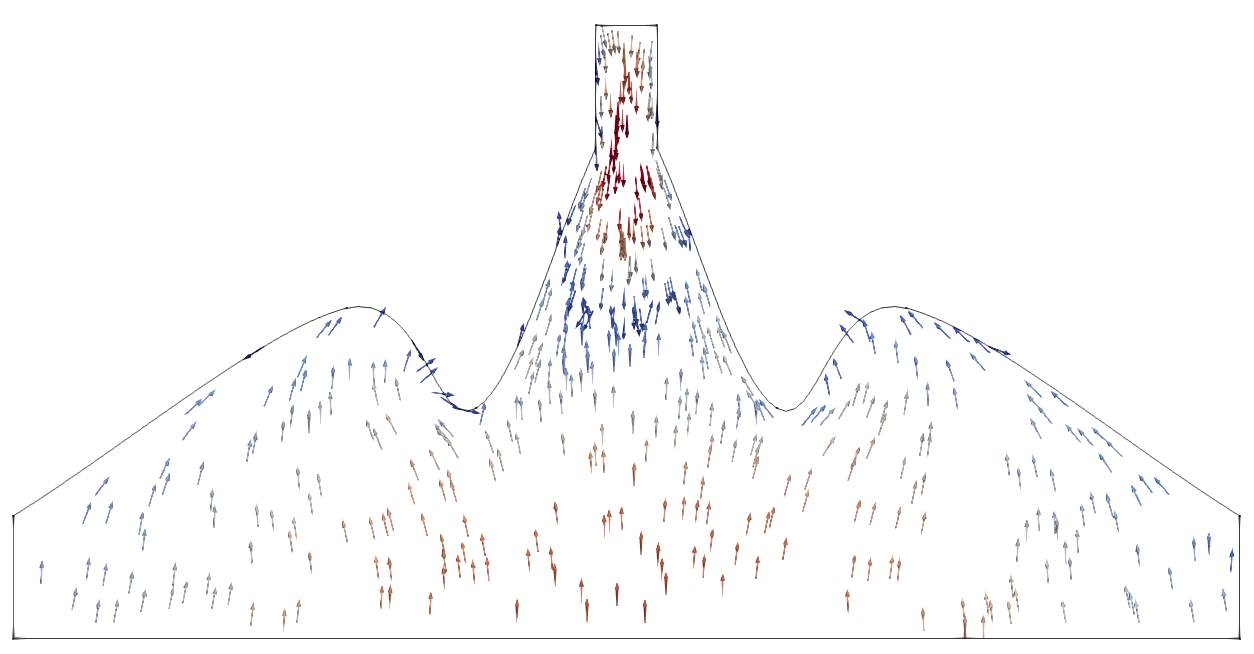
\includegraphics[width=0.96\textwidth]{velocity_field_case_0_s_06_20.png}
        \subcaption{}
    \end{subfigure}
    \begin{subfigure}[b]{0.08\textwidth}
        \centering
        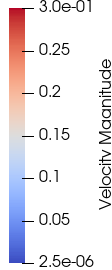
\includegraphics[width=0.96\textwidth]{velocity_field_case_0_s_axis.png}
        \vspace{1.0pt}
    \end{subfigure}
    \\
    \begin{subfigure}[b]{0.30\textwidth}
        \centering
        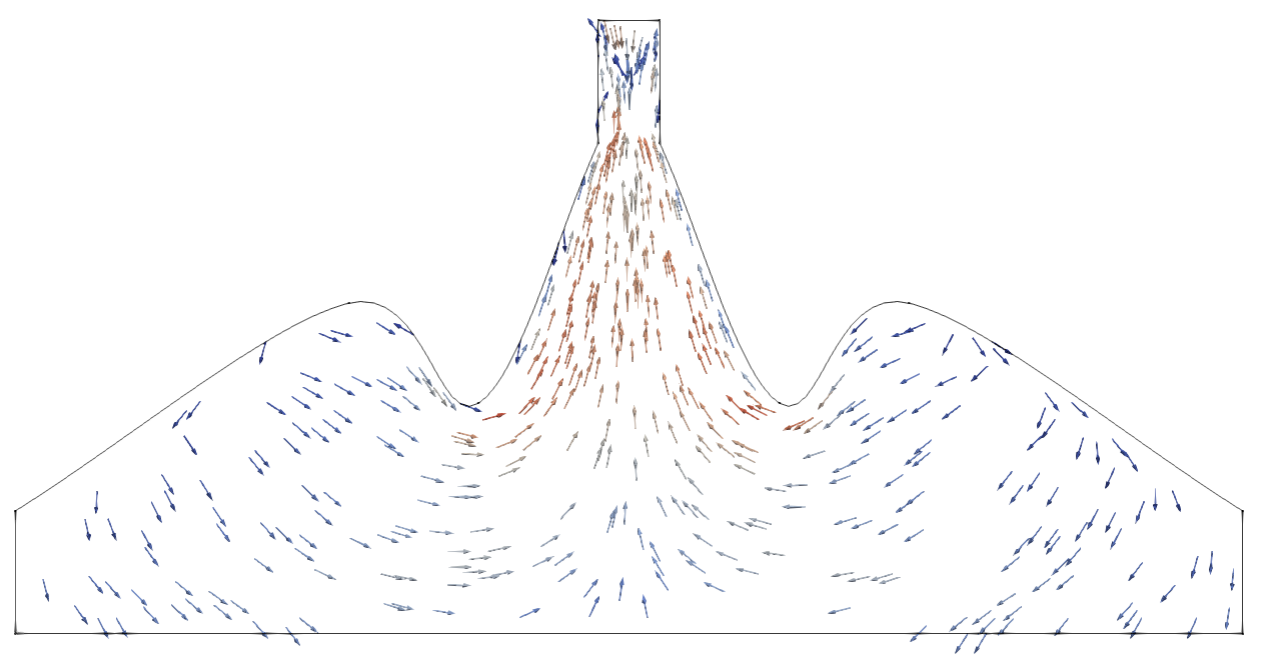
\includegraphics[width=0.96\textwidth]{velocity_field_case_0_s_11_20.png}
        \subcaption{}
    \end{subfigure}
    \begin{subfigure}[b]{0.30\textwidth}
        \centering
        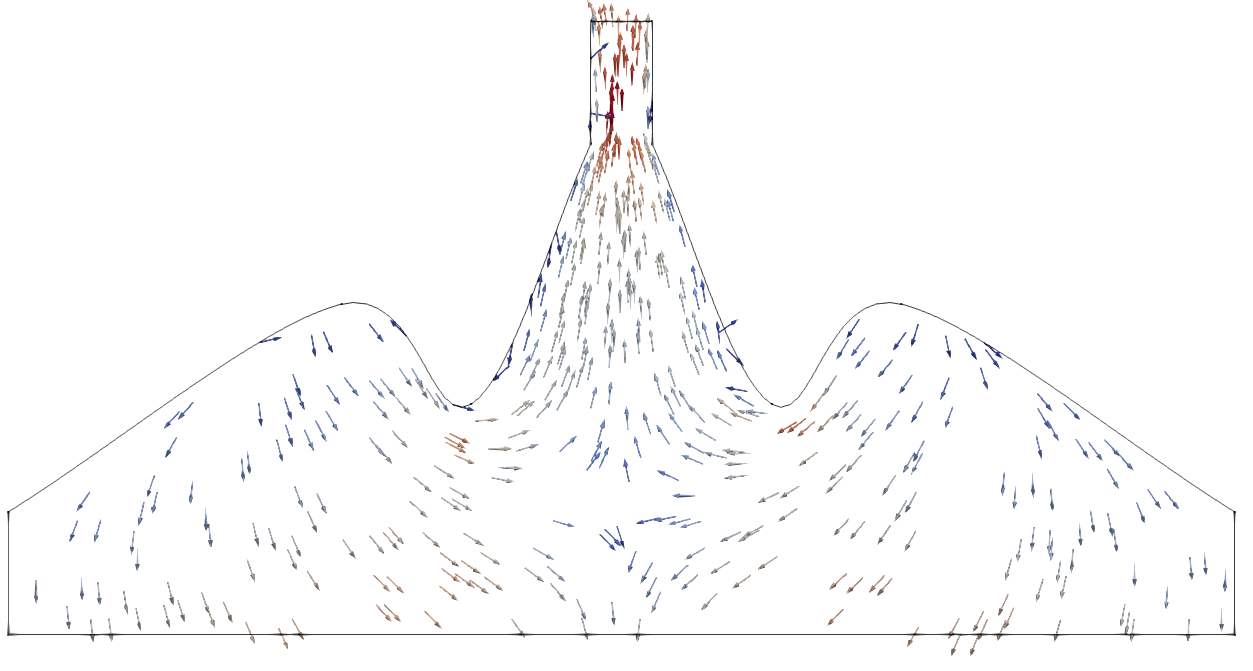
\includegraphics[width=0.96\textwidth]{velocity_field_case_0_s_13_20.png}
        \subcaption{}
    \end{subfigure}
    \begin{subfigure}[b]{0.30\textwidth}
        \centering
        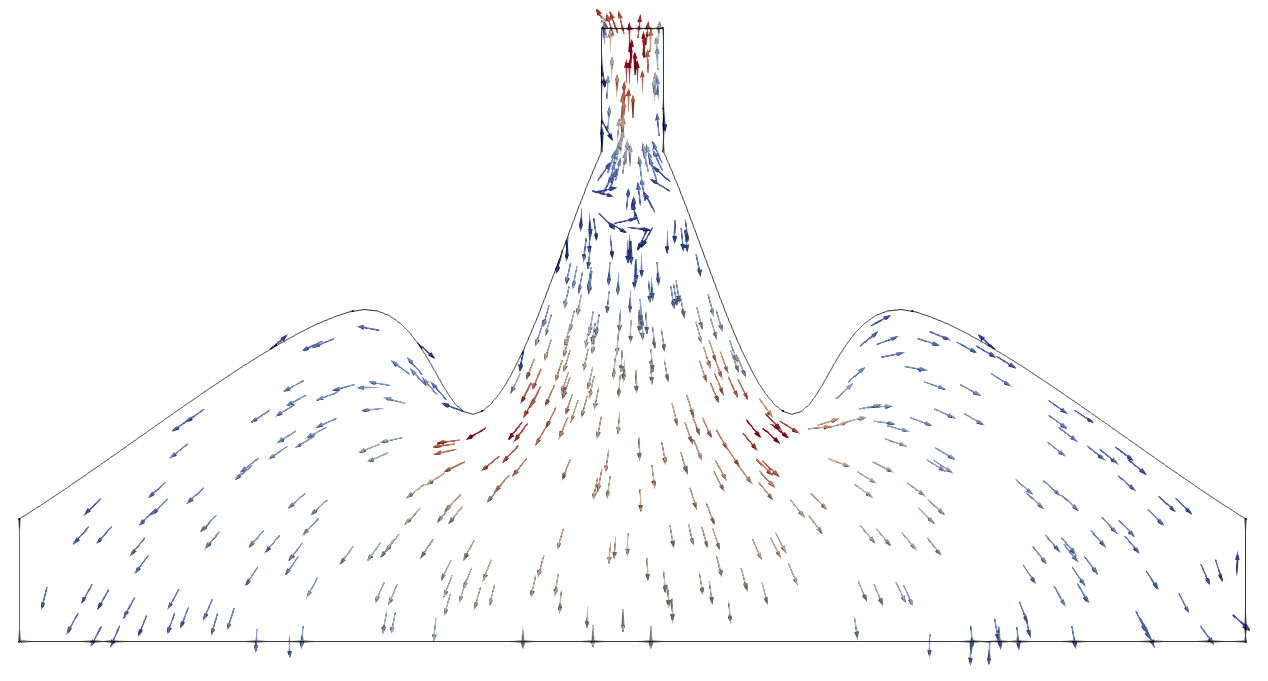
\includegraphics[width=0.96\textwidth]{velocity_field_case_0_s_19_20.png}
        \subcaption{}
    \end{subfigure}
    \captionsetup{font=scriptsize}
    \caption{
    Velocity vector diagrams at 6 time points (a:$\frac{3}{20}T$,b:$\frac{6}{20}T$,c:$\frac{9}{20}T$,d:$\frac{11}{20}T$,e:$\frac{13}{20}T$,f:$\frac{19}{20}T$) during a period for the ``S-shape'' chamber under Case 0.
    Although more fluid collisions occur at the bottom, fluid collisions in the ejection phase are significantly reduced (c)(d).
    Although fluid collisions in the lower part of the chamber are more frequent, there are fewer collisions in the ejection phase (c)(d);
    the fluid velocity in the ``curved pocket'' remains low, serving as a ``fluid buffer zone''.
    }
    \label{fig:velocity_field_case_0_s}
\end{figure}

Summarizing the ``S-shaped'' performance: 1. The ``S-shaped'' also more fully utilizes the pressure-bearing capacity of the lower part of the chamber (Figure \ref{fig:pressure_field_case_0_s}(a)),
but still lacks the pressure dispersion effect of the upper wall in the arched chamber shape. The maximum pressure level is similar to the ``inverted T-shaped'' and ``inverted V-shaped'';
collisions within the ``S-shaped'' chamber mainly occur in the lower part (``curved pockets'' clearly affect upward fluid flow but also result in internal fluid being less affected by downward flow;
fluid velocity in ``curved pockets'' remains low, acting as a fluid buffer zone, so actual kinetic energy loss is not that large).
Mutual collisions between the left and right fluid parts during the ejection phase are not as violent, resulting in smaller energy losses (Figure \ref{fig:velocity_field_case_0_s}(c)(d)).

\subsection{Characteristics of Internal Flow Fields of Derivative Shapes of ``Inverted T-shaped'' and ``S-shaped''}\indent

The pressure cloud map under the derivative shape of the ``inverted T-shaped'' is shown in Figure \ref{fig:pressure_field_case_0_inverted_t_derivative}, and the velocity vector diagram is shown in Figure \ref{fig:velocity_field_case_0_inverted_t_derivative}.

\begin{figure}[htbp]
    \centering
    \begin{subfigure}[b]{0.30\textwidth}
        \centering
        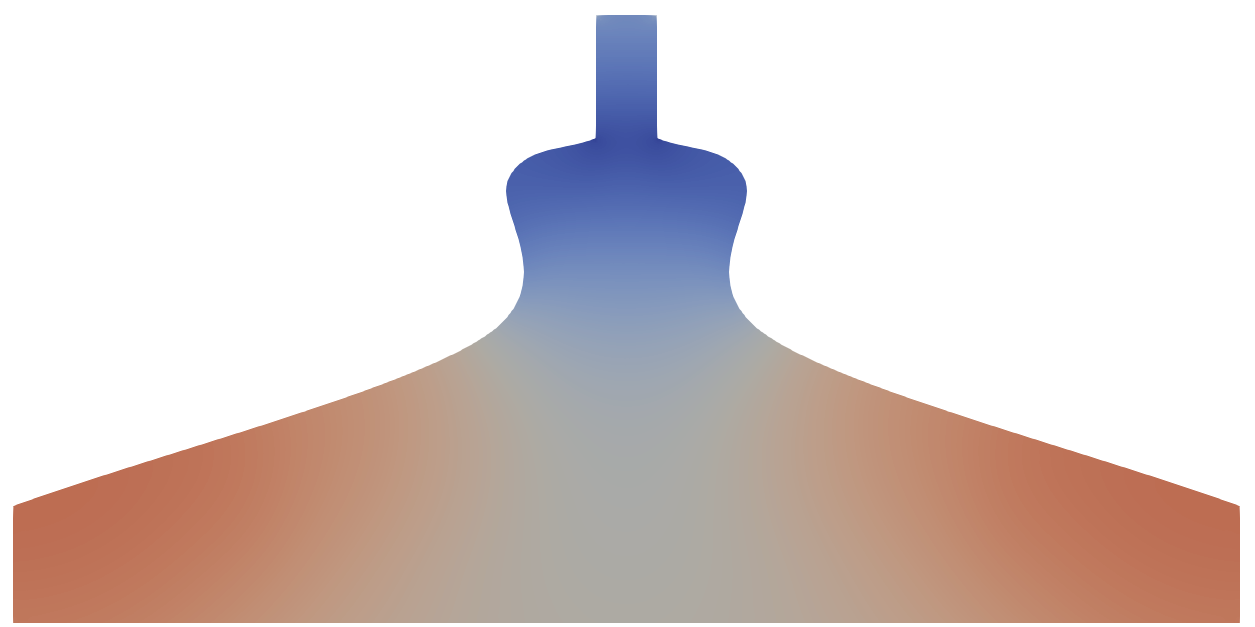
\includegraphics[width=0.96\textwidth]{pressure_field_case_0_inverted_t_derivative_07_20.png}
        \subcaption{}
    \end{subfigure}
    \begin{subfigure}[b]{0.30\textwidth}
        \centering
        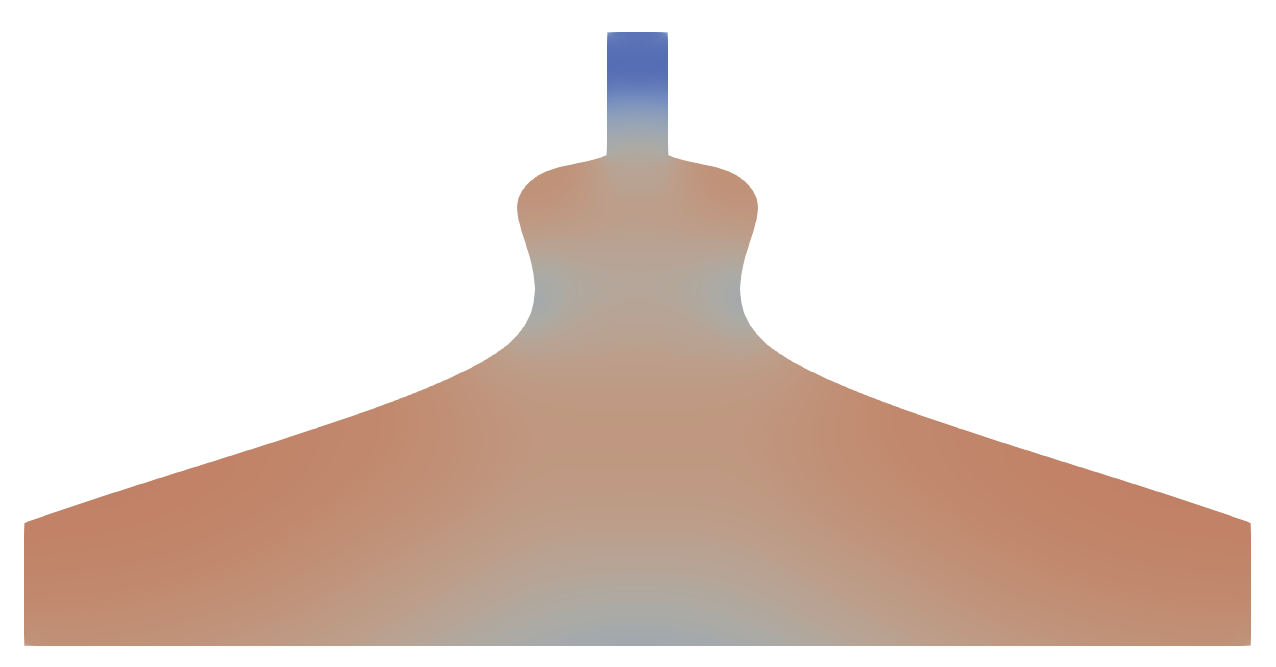
\includegraphics[width=0.96\textwidth]{pressure_field_case_0_inverted_t_derivative_10_20.png}
        \subcaption{}
    \end{subfigure}
    \begin{subfigure}[b]{0.30\textwidth}
        \centering
        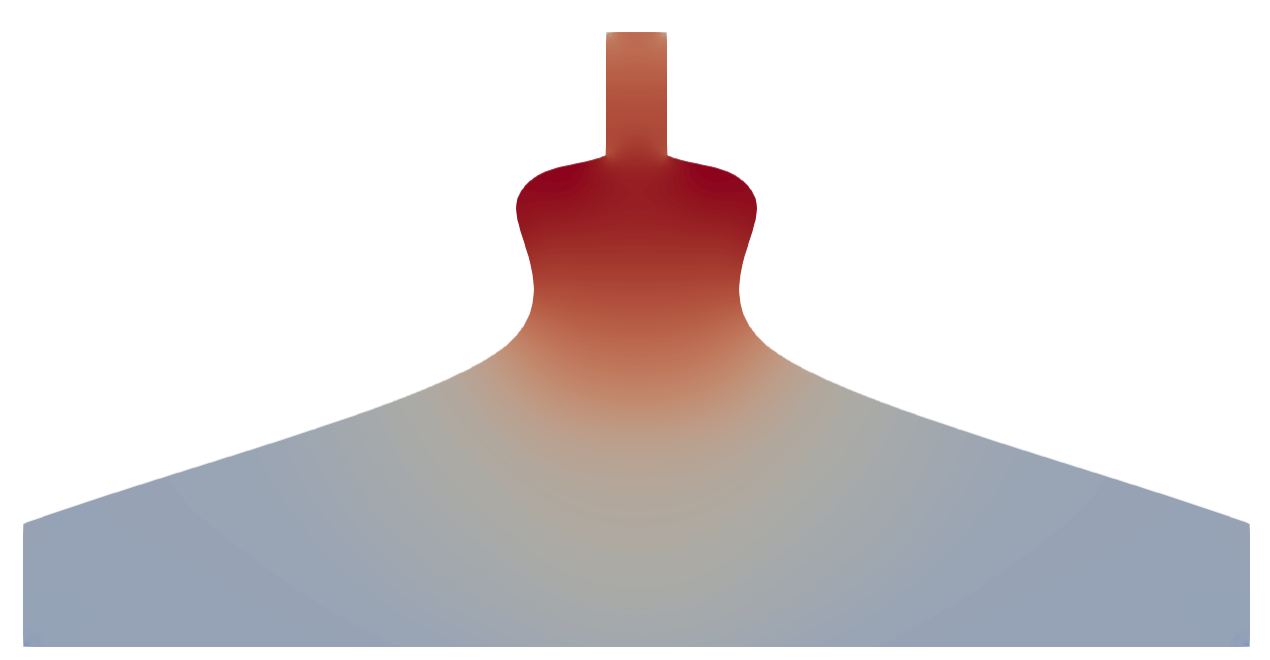
\includegraphics[width=0.96\textwidth]{pressure_field_case_0_inverted_t_derivative_14_20.png}
        \subcaption{}
    \end{subfigure}
    \begin{subfigure}[b]{0.08\textwidth}
        \centering
        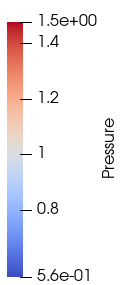
\includegraphics[width=0.96\textwidth]{pressure_field_case_0_inverted_t_derivative_axis.png}
        \subcaption{}
    \end{subfigure}
    \captionsetup{font=scriptsize}
    \caption{
    Pressure contours at 3 time points (a:$\frac{7}{20}T$,b:$\frac{10}{20}T$,c:$\frac{14}{20}T$) during the ``upward push half-cycle'' for the ``inverted T derivative shape'' chamber under Case 0.
    Although the lower part bears greater pressure (a), the maximum pressure appears in the ejection phase (c).
    }
    \label{fig:pressure_field_case_0_inverted_t_derivative}
\end{figure}

\begin{figure}[htbp]
    %\centering
    \begin{subfigure}[b]{0.44\textwidth}
        \centering
        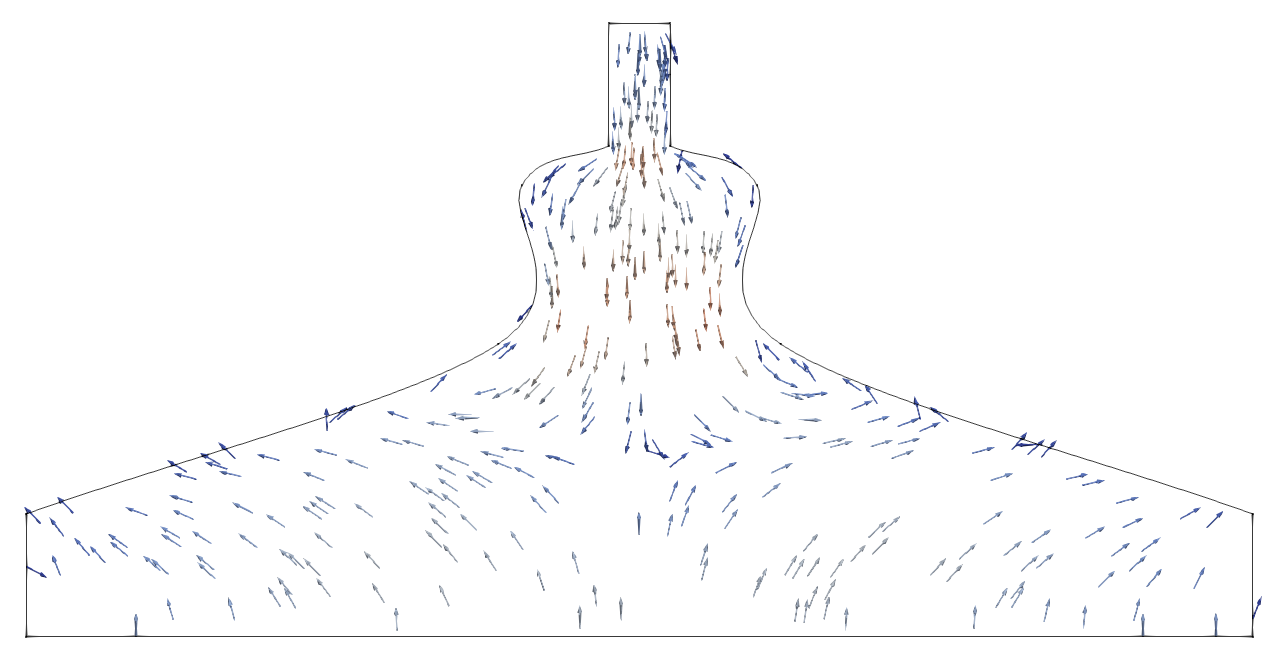
\includegraphics[width=0.96\textwidth]{velocity_field_case_0_inverted_t_derivative_04_20.png}
        \subcaption{}
    \end{subfigure}
    \begin{subfigure}[b]{0.44\textwidth}
        \centering
        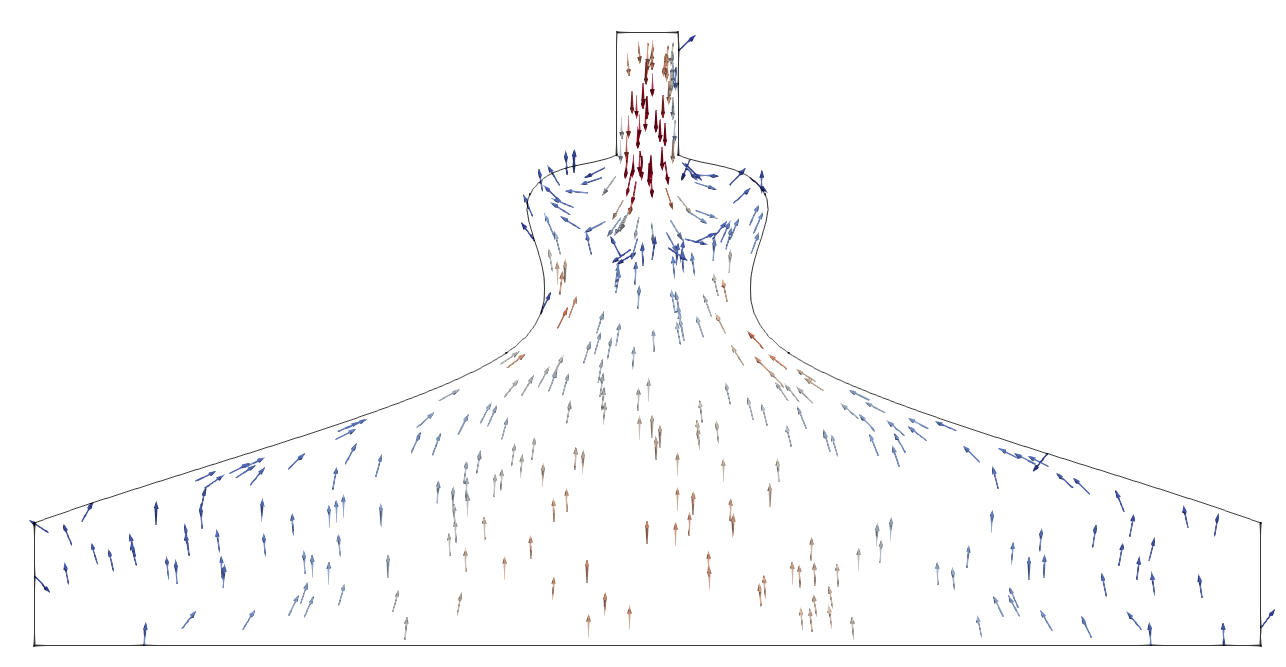
\includegraphics[width=0.96\textwidth]{velocity_field_case_0_inverted_t_derivative_07_20.png}
        \subcaption{}
    \end{subfigure}
    \begin{subfigure}[b]{0.10\textwidth}
        \centering
        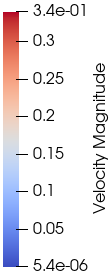
\includegraphics[width=0.96\textwidth]{velocity_field_case_0_inverted_t_derivative_axis.png}
        \vspace{1.0pt}
    \end{subfigure}
    \\
    \begin{subfigure}[b]{0.44\textwidth}
        \centering
        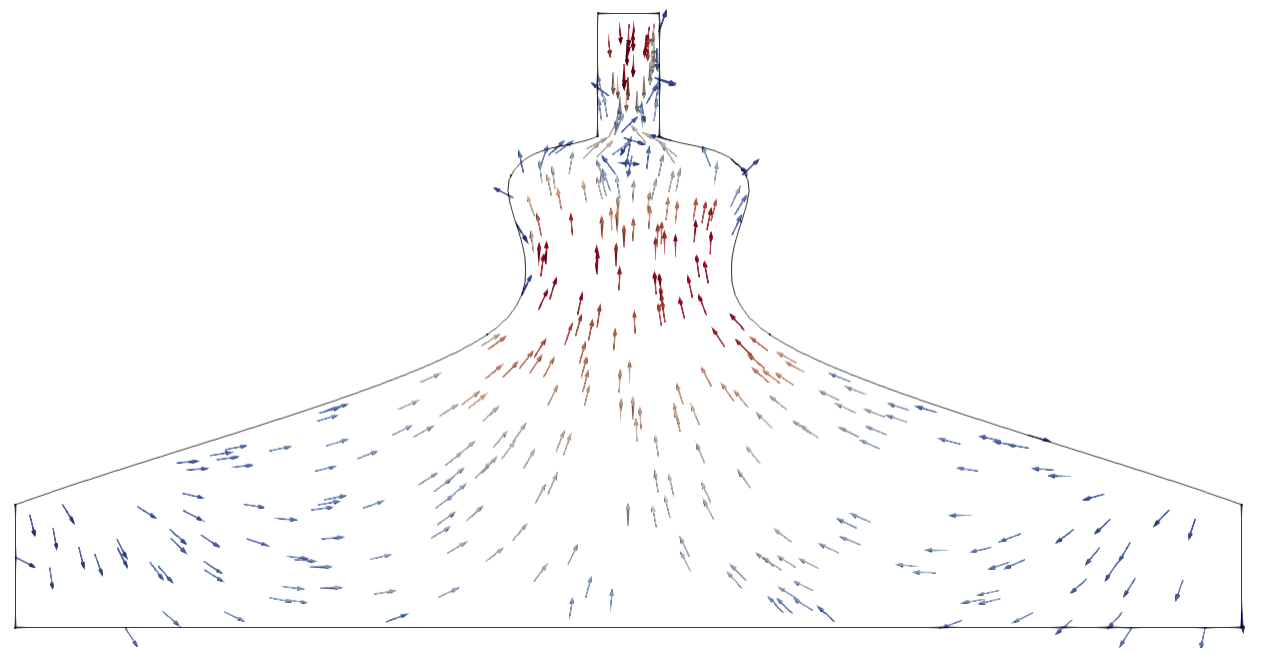
\includegraphics[width=0.96\textwidth]{velocity_field_case_0_inverted_t_derivative_10_20.png}
        \subcaption{}
    \end{subfigure}
    \begin{subfigure}[b]{0.44\textwidth}
        \centering
        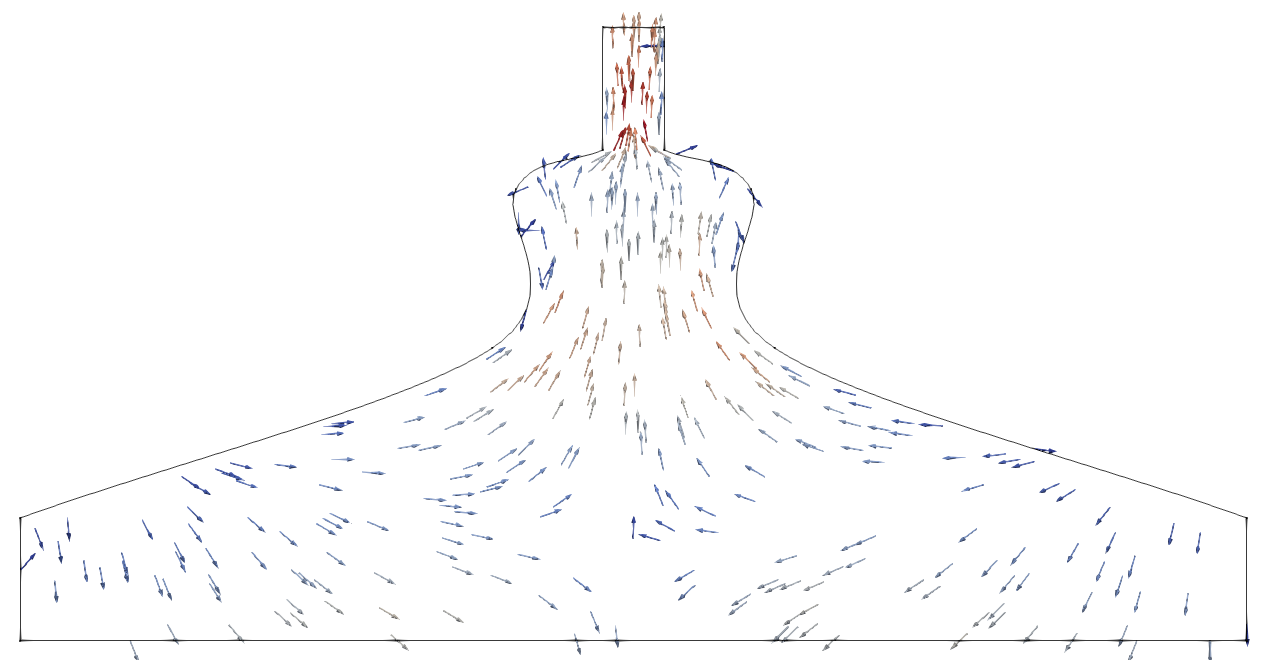
\includegraphics[width=0.96\textwidth]{velocity_field_case_0_inverted_t_derivative_13_20.png}
        \subcaption{}
    \end{subfigure}
    \captionsetup{font=scriptsize}
    \caption{
    Velocity vector diagrams at 4 time points (a:$\frac{4}{20}T$,b:$\frac{7}{20}T$,c:$\frac{10}{20}T$,d:$\frac{13}{20}T$) during the ``upward push half-cycle'' for the ``inverted T derivative shape'' chamber under Case 0.
    Although fluid collisions within the lower part of the chamber are stronger (weaker relative to the ``inverted T-shaped''), fluid collisions in the ejection phase are weaker (stronger relative to the ``inverted T-shaped'')(c)(d).
    }
    \label{fig:velocity_field_case_0_inverted_t_derivative}
\end{figure}

Compared to the ``inverted T-shaped'', this derivative shape mainly widens the original ``narrow channel'' connected to the top outlet.
The derivative shape also more fully utilizes the pressure-bearing capacity of the lower chamber (Figure \ref{fig:pressure_field_case_0_inverted_t_derivative}(a)),
lacks the pressure dispersion effect of the upper part of convex walls, and the maximum pressure appears at the ejection moment (Figure \ref{fig:pressure_field_case_0_inverted_t_derivative}(c))
(widening the channel connected to the top outlet should have the potential to further reduce maximum pressure compared to the ``inverted T-shaped'', however, data does not prove this);
mutual collisions of fluid within the chamber and collisions between fluid and chamber walls still occur mainly in the lower chamber;
widening the part near the outlet might have reduced fluid collisions in the lower chamber but also intensified collisions in the ejection phase (Figure \ref{fig:velocity_field_case_0_inverted_t_derivative}(c)(d)).
Finally, this type of derivative ``inverted T-shaped'' shape achieved wall pressure and outlet velocity performance similar to the ``inverted T-shaped''.

The pressure cloud map under the ``S-shaped'' derivative shape is shown in Figure \ref{fig:pressure_field_case_0_s_derivative}, and the velocity vector diagram is shown in Figure \ref{fig:velocity_field_case_0_s_derivative}.
This ``S-shaped'' derivative shape combines characteristics of the ``S-shaped'' and ``inverted T-shaped''.
This derivative shape simultaneously utilizes the pressure-bearing capacity of the ``horizontal step'' in the lower part and the ``curved pocket'' in the middle (Figure \ref{fig:pressure_field_case_0_s_derivative}(a)(b)),
lacks a gentle upper part like the arched chamber, and the maximum pressure is slightly higher than the arched chamber.
During the upward fluid push, it is less affected by the ``horizontal step'';
guided by the ``horizontal step'' in the lower part, the fluid is also less affected by the ``curved pocket''; fluid collisions are minimal at the ejection moment (Figure \ref{fig:velocity_field_case_0_s_derivative}(c)(d)).
Ultimately, this ``S-shaped'' derivative shape balances features of both ``S-shaped'' and ``T-shaped'' and its actual performance is similar to both.

\begin{figure}[htbp]
    \centering
    \begin{subfigure}[b]{0.30\textwidth}
        \centering
        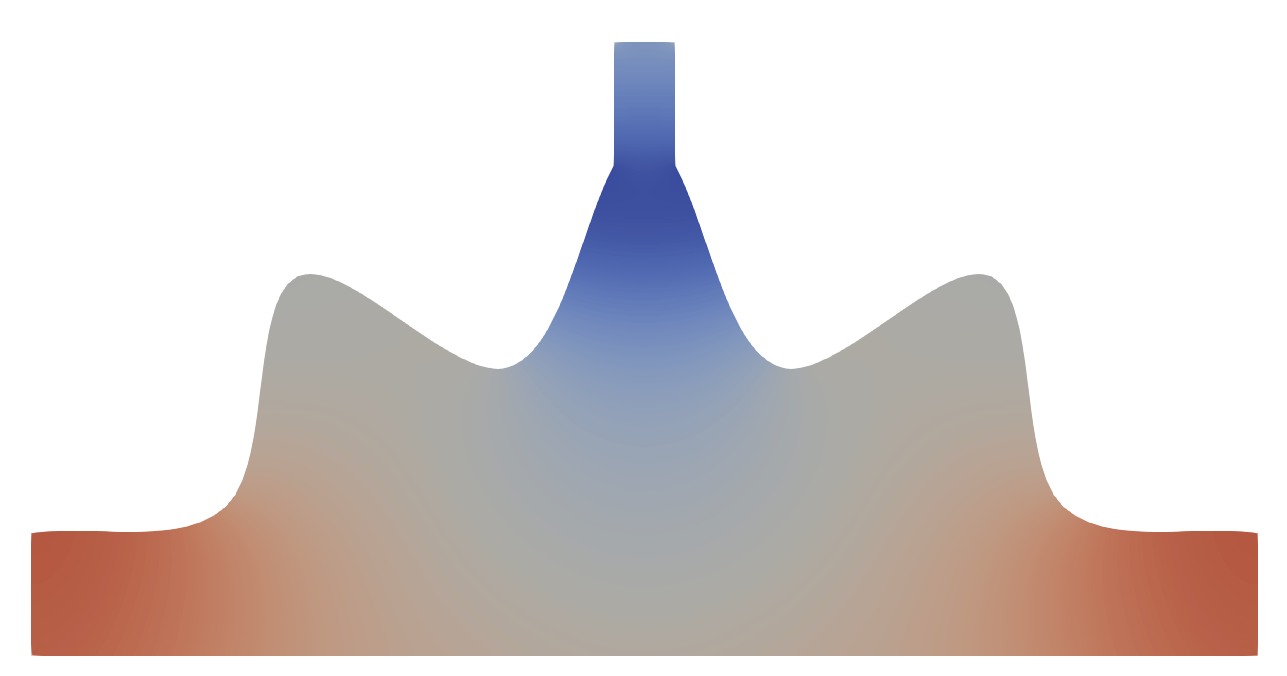
\includegraphics[width=0.96\textwidth]{pressure_field_case_0_s_derivative_06_20.png}
        \subcaption{}
    \end{subfigure}
    \begin{subfigure}[b]{0.30\textwidth}
        \centering
        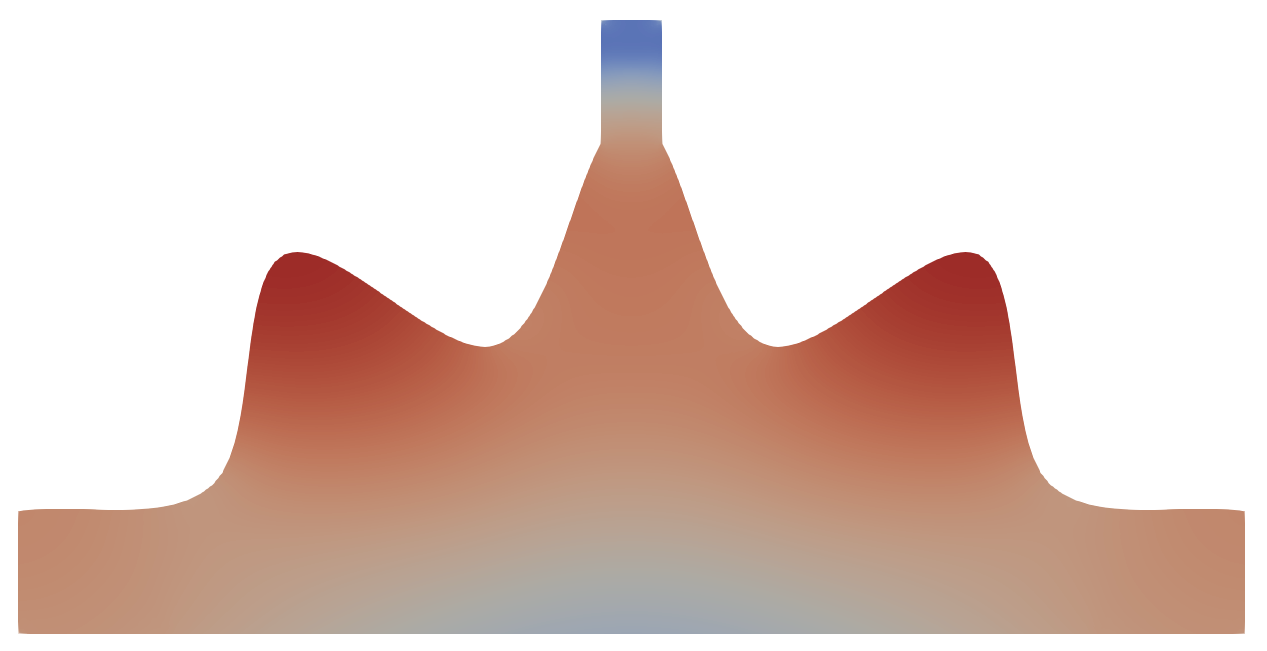
\includegraphics[width=0.96\textwidth]{pressure_field_case_0_s_derivative_10_20.png}
        \subcaption{}
    \end{subfigure}
    \begin{subfigure}[b]{0.30\textwidth}
        \centering
        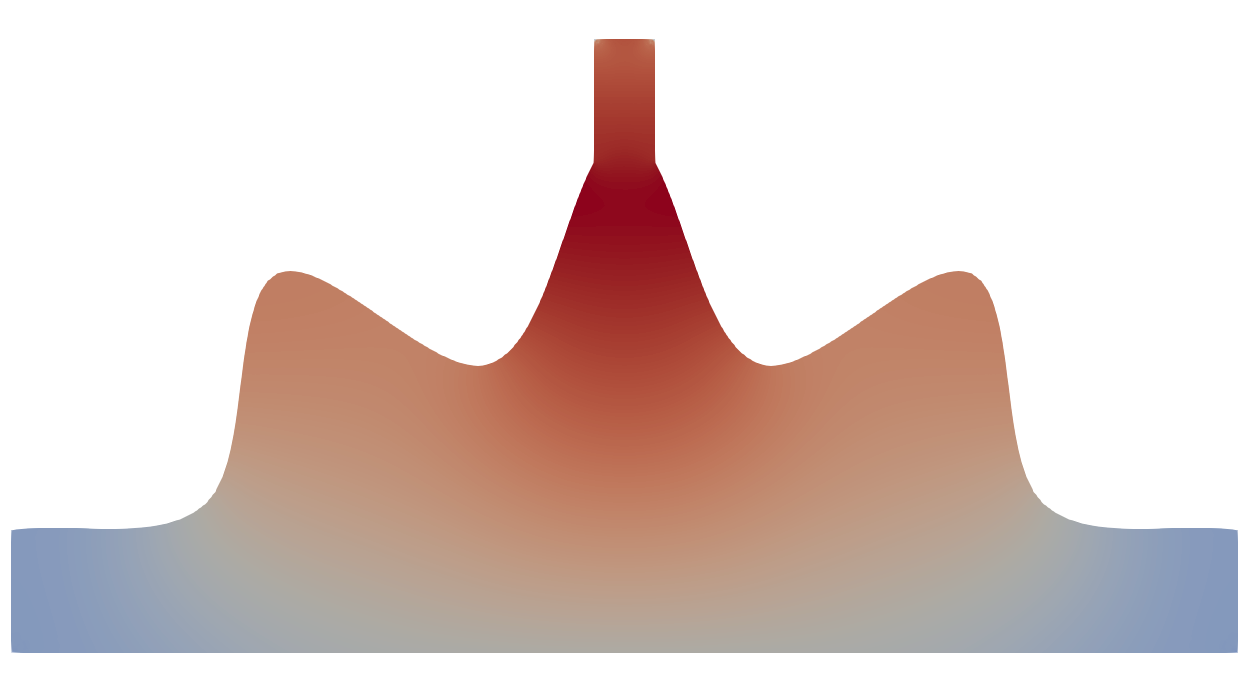
\includegraphics[width=0.96\textwidth]{pressure_field_case_0_s_derivative_14_20.png}
        \subcaption{}
    \end{subfigure}
    \begin{subfigure}[b]{0.08\textwidth}
        \centering
        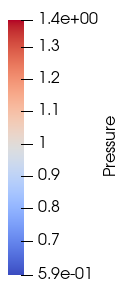
\includegraphics[width=0.96\textwidth]{pressure_field_case_0_s_derivative_axis.png}
        \subcaption{}
    \end{subfigure}
    \captionsetup{font=scriptsize}
    \caption{
    Pressure contours at 3 time points (a:$\frac{6}{20}T$,b:$\frac{10}{20}T$,c:$\frac{14}{20}T$) during the ``upward push half-cycle'' for the ``S derivative shape'' chamber under Case 0.
    Simultaneously utilizes the pressure-bearing capacity of the ``horizontal step'' at the bottom and the ``curved pocket'' (a)(b), the maximum pressure appears at the ejection moment (c).
    }
    \label{fig:pressure_field_case_0_s_derivative}
\end{figure}

\begin{figure}[htbp]
    %\centering
    \begin{subfigure}[b]{0.44\textwidth}
        \centering
        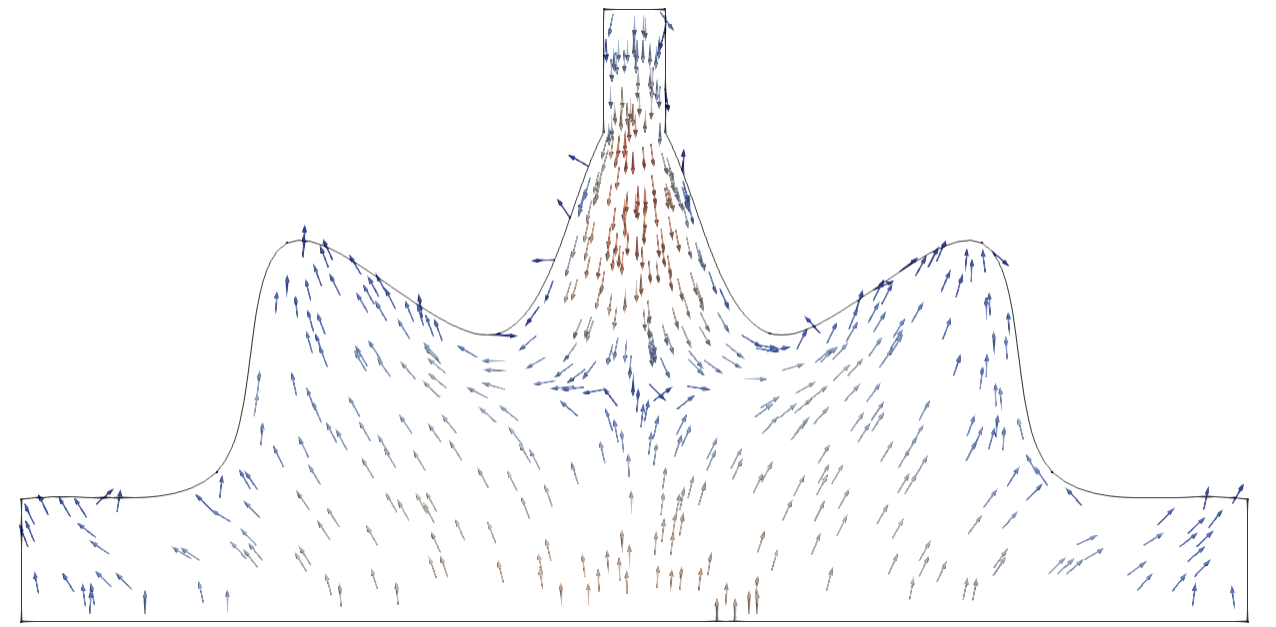
\includegraphics[width=0.96\textwidth]{velocity_field_case_0_s_derivative_04_20.png}
        \subcaption{}
    \end{subfigure}
    \begin{subfigure}[b]{0.44\textwidth}
        \centering
        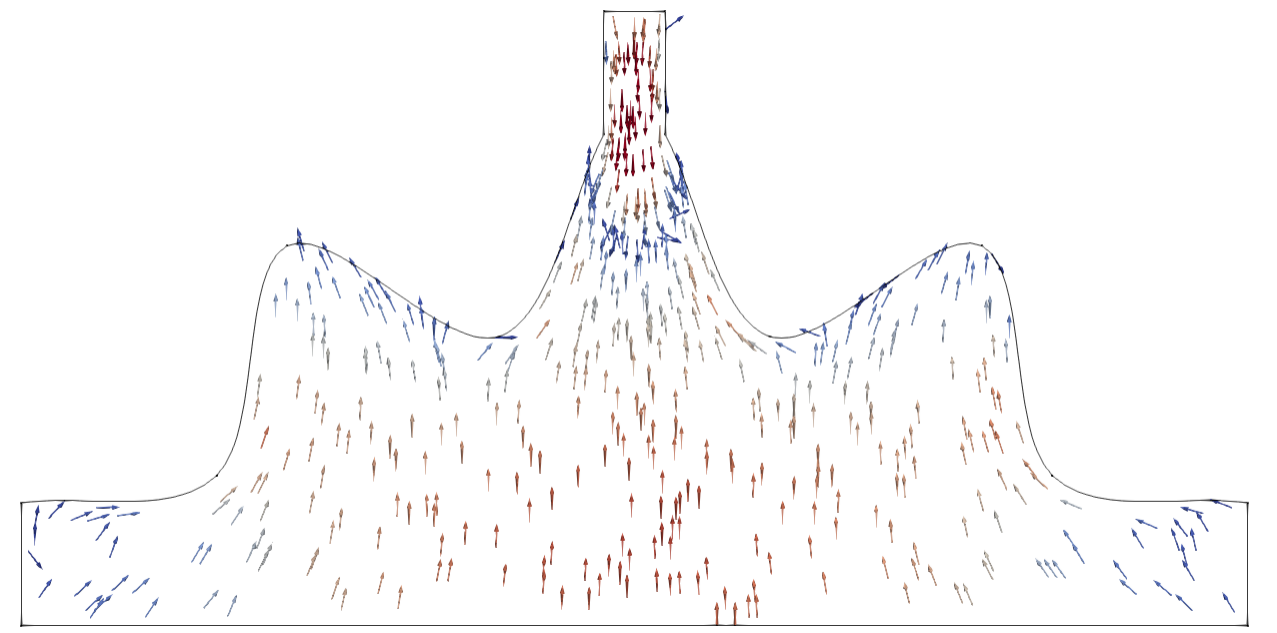
\includegraphics[width=0.96\textwidth]{velocity_field_case_0_s_derivative_07_20.png}
        \subcaption{}
    \end{subfigure}
    \begin{subfigure}[b]{0.10\textwidth}
        \centering
        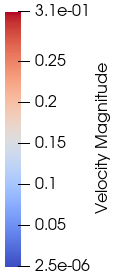
\includegraphics[width=0.96\textwidth]{velocity_field_case_0_s_derivative_axis.png}
        \vspace{1.0pt}
    \end{subfigure}
    \\
    \begin{subfigure}[b]{0.44\textwidth}
        \centering
        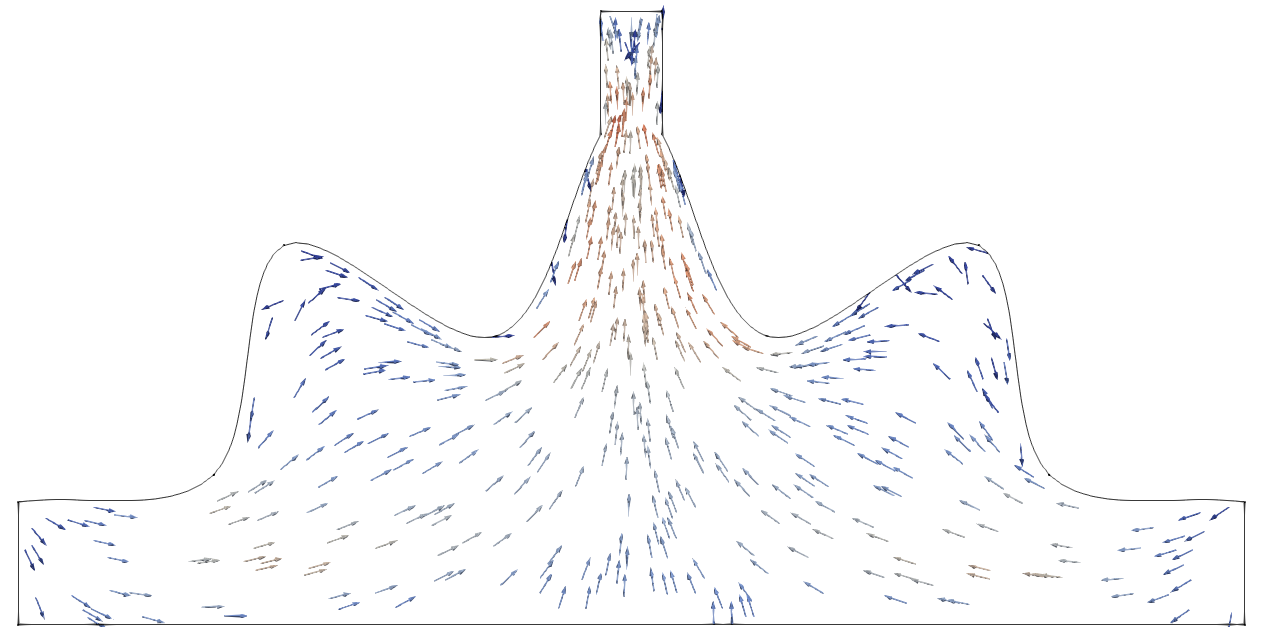
\includegraphics[width=0.96\textwidth]{velocity_field_case_0_s_derivative_11_20.png}
        \subcaption{}
    \end{subfigure}
    \begin{subfigure}[b]{0.44\textwidth}
        \centering
        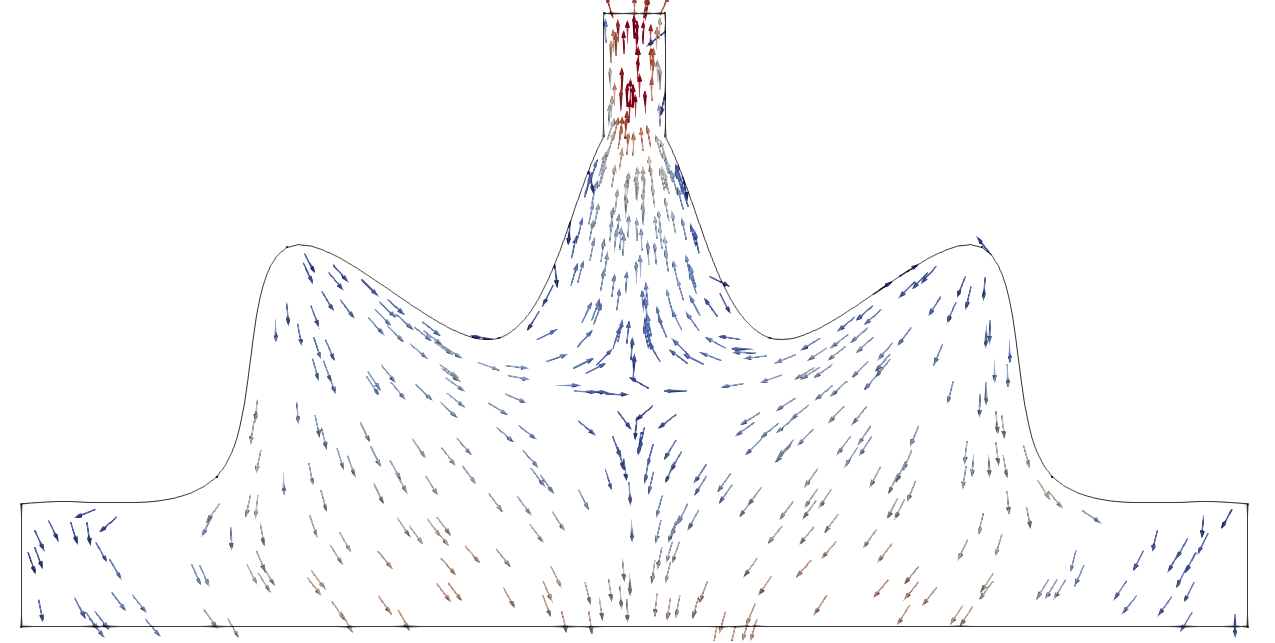
\includegraphics[width=0.96\textwidth]{velocity_field_case_0_s_derivative_14_20.png}
        \subcaption{}
    \end{subfigure}
    \captionsetup{font=scriptsize}
    \caption{
    Velocity vector diagrams at 4 time points (a:$\frac{4}{20}T$,b:$\frac{7}{20}T$,c:$\frac{11}{20}T$,d:$\frac{14}{20}T$) during the ``upward push half-cycle'' for the ``S derivative shape'' chamber under Case 0.
    Fluid collisions at the bottom and the ``curved pocket'' are weaker compared to both ``inverted T-shaped'' and ``S-shaped'', but exist in both; collisions in the ejection phase are weaker (c)(d).
    }
    \label{fig:velocity_field_case_0_s_derivative}
\end{figure}

\subsection{Tentative Analysis of the Difficulty in Obtaining ``Inverted V-shaped'' Chamber Shapes in Training}\indent

Brief summary of ``inverted T-shaped'' and ``S-shaped'' chamber shapes:
``Inverted T-shaped'' and ``S-shaped'' chamber shapes appropriately increase the pressure borne by the bottom wall during the upward fluid push,
causing more fluid collisions and kinetic energy dissipation in the bottom area, in exchange for fewer fluid collisions and energy losses during the ejection phase.
Ultimately, ``inverted T-shaped'' and ``S-shaped'' achieve performance similar to the more traditional ``inverted V-shaped''.

After analyzing these shapes, the end of this chapter attempts to answer one question:
Since ``inverted T-shaped'', ``S-shaped'', and ``inverted V-shaped'' have similar performance,
why does the reinforcement learning algorithm prefer the first two and rarely give the ``inverted V-shaped''?

To form ``inverted T-shaped'' and ``S-shaped'' chamber shapes, the positions of control points are relatively fixed (Figure \ref{fig:control_point_example_t_s}).

\begin{figure}[htbp]
    \centering
    \begin{subfigure}[b]{0.32\textwidth}
        \centering
        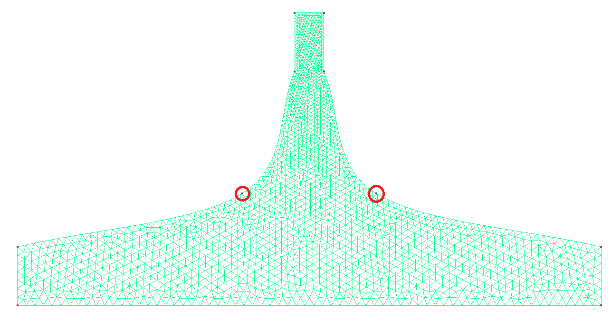
\includegraphics[width=0.96\textwidth]{control_point_example_inverted_t.png}
        \subcaption{}
    \end{subfigure}
    \begin{subfigure}[b]{0.32\textwidth}
        \centering
        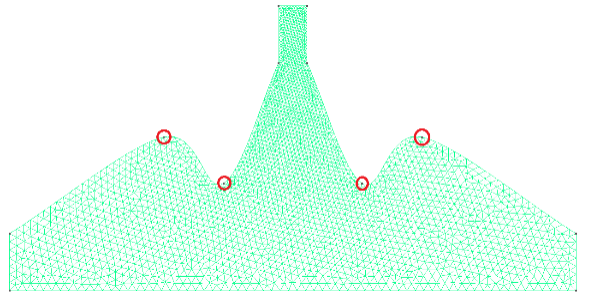
\includegraphics[width=0.96\textwidth]{control_point_example_s.png}
        \subcaption{}
    \end{subfigure}
    \captionsetup{font=scriptsize}
    \caption{
    Control point examples for chamber shapes.
    Points within red circles are wall curve control points.
    (a) Requirements for ``inverted T-shaped''; (b) Requirements for ``S-shaped'';
    Agent learning these shapes needs to select points at specific positions.
    }
    \label{fig:control_point_example_t_s}
\end{figure}

To form an ``inverted V-shaped'' wall, the Agent needs to select one or more control points roughly on the line segment between the bottom velocity inlet endpoint and the top outlet endpoint (Figure \ref{fig:control_point_example_v}).

\begin{figure}[htbp]
    \centering
    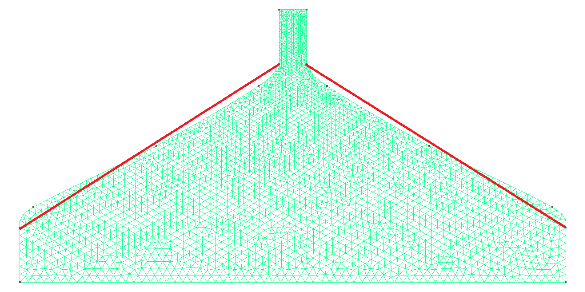
\includegraphics[width=0.32\textwidth]{control_point_example_inverted_v.png}
    \captionsetup{font=scriptsize}
    \caption{
    Control point examples for the ``inverted V'' shape.
    Points within red circles are wall curve control points.
    Agent learning this requires selected control points to follow a straight-line rule rather than just picking points.
    Researchers speculate this is harder.
    }
    \label{fig:control_point_example_v}
\end{figure}

To get ``inverted T-shaped'' and ``S-shaped'', the Agent needs to learn how to select 1 or more control points within a specific range;
to get ``inverted V-shaped'', the Agent needs to learn to select 1 or more control points in a larger range that satisfy the rule of sequential distribution on a straight line.
It is speculated that selecting control points in a smaller range is easier than selecting points in a larger range that sequentially align on a straight line.
This phenomenon may reflect the difference in thinking between researchers and reinforcement learning algorithms.
These distinct chamber shapes and the analysis of their optimization mechanisms may help future research and applications.

\subsection{Analysis and Comparison of Optimization Schemes under Other Physical Parameters}\indent

Although ``inverted T-shaped'', ``S-shaped'', and ``inverted V-shaped'' obtained under Case 0 were analyzed,
this paper hopes to further understand their applicability under other physical parameters.
Results for whether they remain optimized shapes under other parameters are summarized in Table \ref{tab:whether_inverted_t_and_s_are_optimized_shapes_in_cases}.
Except for doubled amplitude and frequency (where flow laws and optimization mechanisms differ), ``inverted T-shaped'' shows a wider range of applicability; ``S-shaped'' seems to have some geometric dependency.

\begin{table}[h]
    \centering
    \caption{Whether Inverted T and S are optimized shapes in cases}
    \label{tab:whether_inverted_t_and_s_are_optimized_shapes_in_cases}
    \begin{tabular}{c c c}
        \hline
        \hline
        {Case}&{Inverted T as optimized}&{S as optimized}\\
        \hline
        {Case 0}&{1}&{1}\\
        \hline
        {Case 1(half chamber height)}&{1}&{0}\\
        \hline
        {Case 2(double chamber height)}&{1}&{1}\\
        \hline
        {Case 3(half amplitude)}&{1}&{0}\\
        \hline
        {Case 4(double amplitude)}&{0}&{0}\\
        \hline
        {Case 5(half frenquency)}&{1}&{0}\\
        \hline
        {Case 6(double frenquency)}&{0}&{0}\\
        \hline
        {Case 7(half unit size)}&{1}&{0}\\
        \hline
        {Case 8(double unit size)}&{1}&{1}\\
        \hline
        \hline
    \end{tabular}
\end{table}

Summary of results for different parameters: 1. ``Inverted V-shaped'' and ``S-shaped'' can still be obtained under other parameters and show similar performance, especially under height changes, half amplitude, and half frequency;
2. Under double amplitude and double period, fluid motion laws change, results are no longer ``inverted T'' or ``S'', and optimization mechanisms differ;
3. Even when they are optimized, ``inverted T'' appears more often; ``S-shaped'' appears less and seems geometry-dependent (Table \ref{tab:whether_inverted_t_and_s_are_optimized_shapes_in_cases}).
Details for Case 1, 2, 3, 5, 7, 8 are in the appendix.
Focus here is on double amplitude and double frequency.

Data from Case 0 reflects that smooth transition of ``inverted V-shaped'' might not have a huge impact.
In subsequent cases, straight walls or ``trapezoidal'' chambers are used as references.

Case 4 only doubles amplitude. Shapes obtained are mainly arched (Figure \ref{fig:optimized_shapes_case_4}).

\begin{figure}[htbp]
    \centering
    \begin{subfigure}[b]{0.32\textwidth}
        \centering
        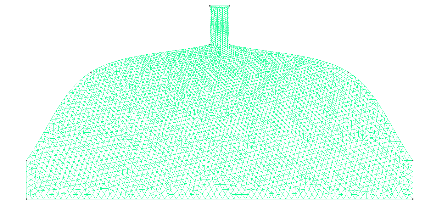
\includegraphics[width=0.96\textwidth]{optimized_shape_case_4_arched_1_conrol_point.png}
        \subcaption{}
    \end{subfigure}
    \begin{subfigure}[b]{0.32\textwidth}
        \centering
        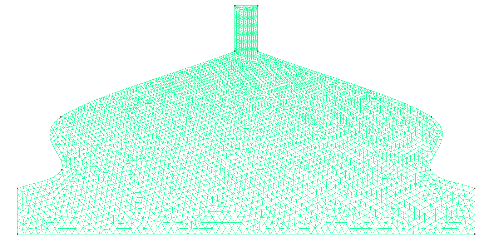
\includegraphics[width=0.96\textwidth]{optimized_shape_case_4_arched_2_conrol_points.png}
        \subcaption{}
    \end{subfigure}
    \captionsetup{font=scriptsize}
    \caption{
    Arched shapes in Case 4 using (a) 1 control point or (b) 2 control points.
    Flow fields are similar, only (a) is analyzed.
    }
    \label{fig:optimized_shapes_case_4}
\end{figure}

\begin{figure}[htbp]
    \centering
    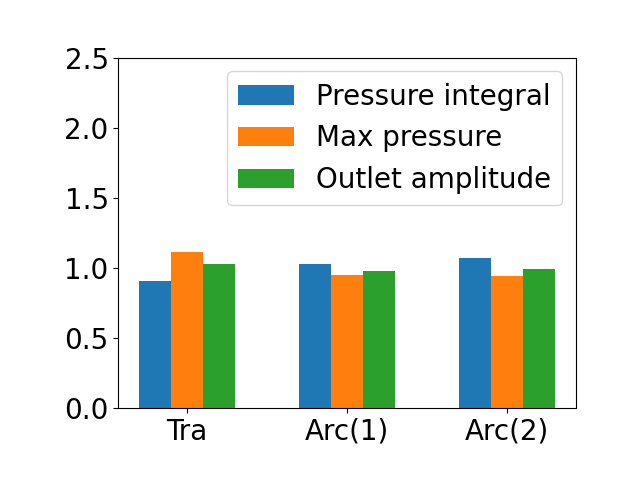
\includegraphics[width=0.64\textwidth]{target_data_case_4.png}
    \captionsetup{font=scriptsize}
    \caption{
    Target data for optimized shapes under Case 4.
    At higher amplitudes, the optimized shapes are no longer ``inverted T'' or ``S'', showing obvious advantages over trapezoidal chambers.
    }
    \label{fig:target_data_of_optimized_shapes_case_4}
\end{figure}

Combined with Figure \ref{fig:target_data_of_optimized_shapes_case_4}, optimized shapes mainly significantly reduce maximum wall pressure without affecting outlet velocity amplitude much.
Shapes are neither ``inverted T'' nor ``inverted V''. Arched shapes with 1 vs 2 control points have slight differences but basic flow characteristics are similar.
Next, compare pressure cloud maps and velocity vectors of ``trapezoidal'' vs 1-control-point ``arched'' chambers.
Selection of pressure results for Case 4 is similar to Case 0: moments showing different pressure levels on the wall;
for velocity: moments showing interaction between incoming, downward flow, walls, and ejection phase.
Case 4 focuses on pressure wave divergence in the ejection phase (Figure \ref{fig:pressure_field_case_4_trapezoidal}(c)(d)).

\begin{figure}[htbp]
    %\centering
    \begin{subfigure}[b]{0.44\textwidth}
        \centering
        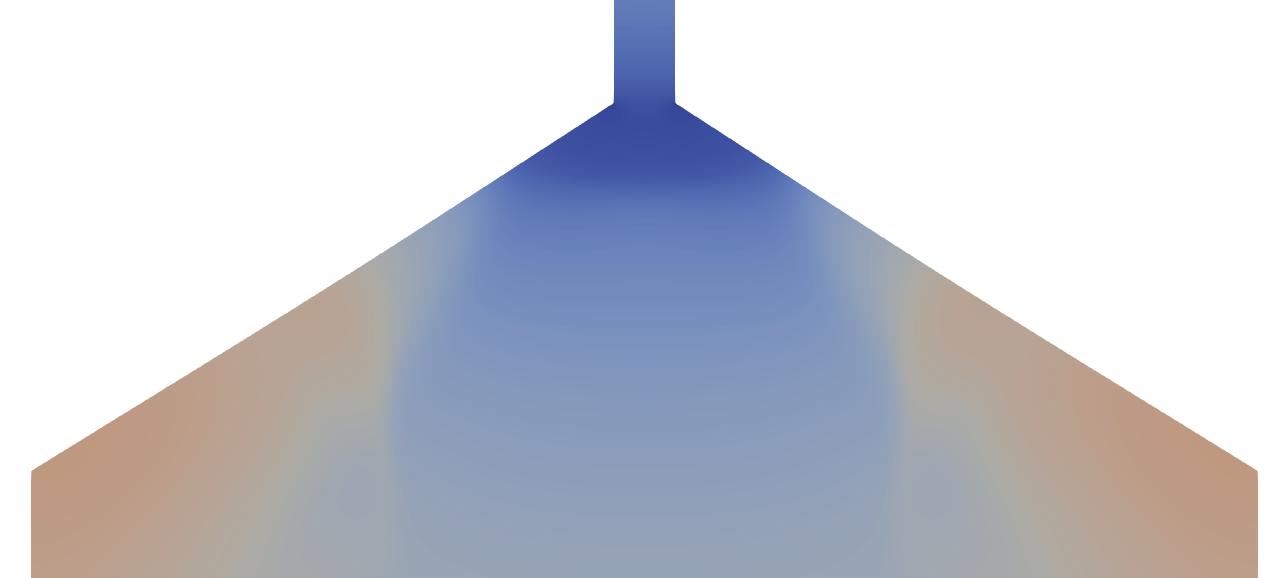
\includegraphics[width=0.96\textwidth]{pressure_field_case_4_trapezoidal_07_20.png}
        \subcaption{}
    \end{subfigure}
    \begin{subfigure}[b]{0.44\textwidth}
        \centering
        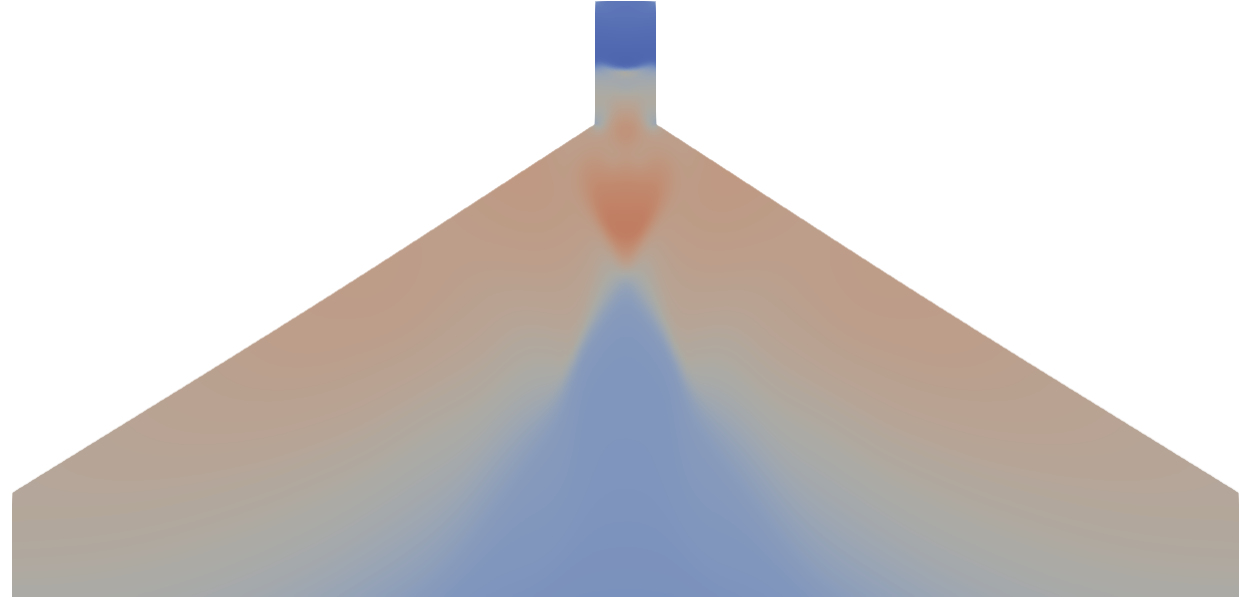
\includegraphics[width=0.96\textwidth]{pressure_field_case_4_trapezoidal_10_20.png}
        \subcaption{}
    \end{subfigure}
    \begin{subfigure}[b]{0.10\textwidth}
        \centering
        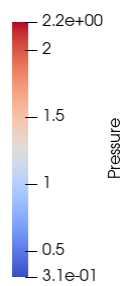
\includegraphics[width=0.96\textwidth]{pressure_field_case_4_trapezoidal_axis.png}
        \vspace{1.0pt}
    \end{subfigure}
    \\
    \begin{subfigure}[b]{0.44\textwidth}
        \centering
        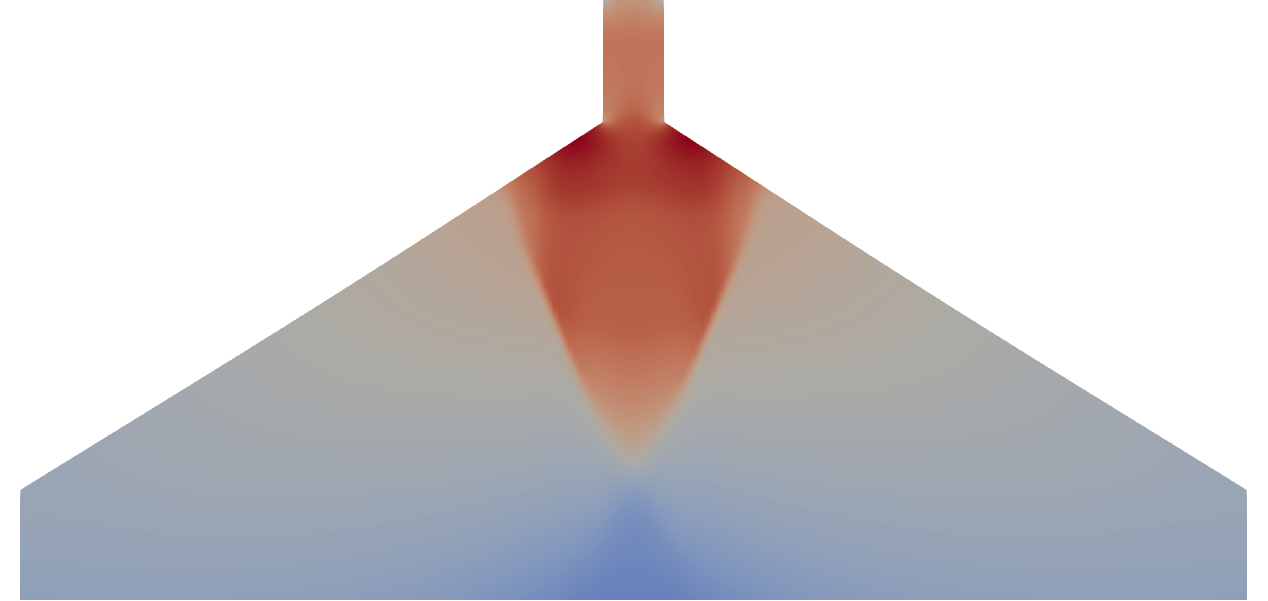
\includegraphics[width=0.96\textwidth]{pressure_field_case_4_trapezoidal_12_20.png}
        \subcaption{}
    \end{subfigure}
    \begin{subfigure}[b]{0.44\textwidth}
        \centering
        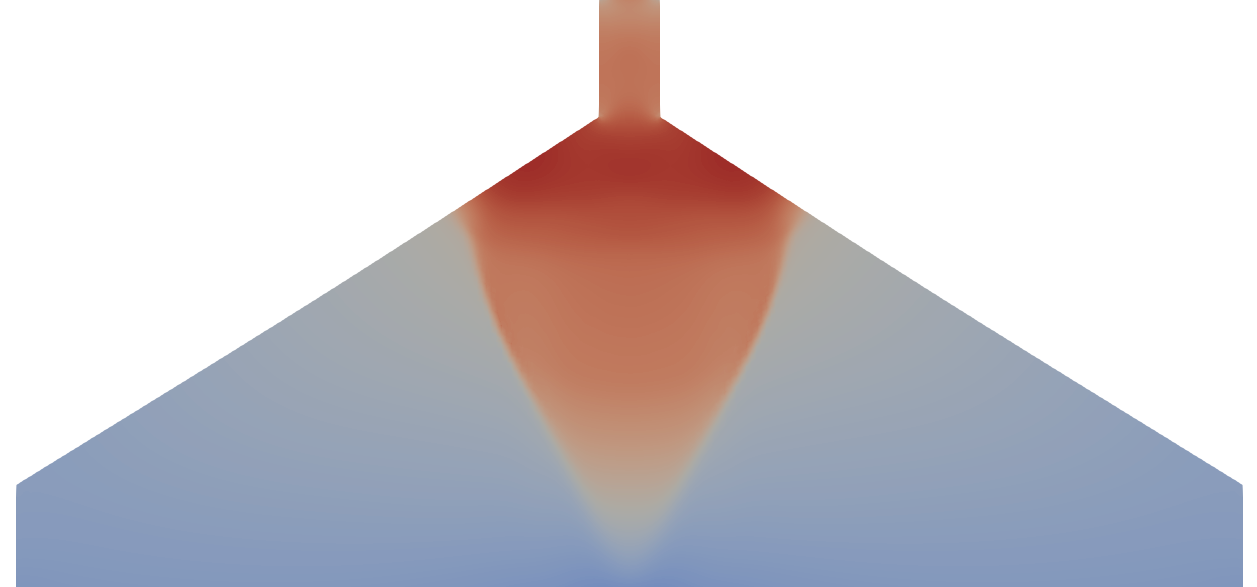
\includegraphics[width=0.96\textwidth]{pressure_field_case_4_trapezoidal_13_20.png}
        \subcaption{}
    \end{subfigure}
    \captionsetup{font=scriptsize}
    \caption{
    Pressure contours at 4 time points (a:$\frac{7}{20}T$,b:$\frac{12}{20}T$,c:$\frac{13}{20}T$) during the ``upward push half-cycle'' for the trapezoidal chamber under Case 4.
    Violent collisions and diverging pressure waves in ejection phase (c)(d).
    }
    \label{fig:pressure_field_case_4_trapezoidal}
\end{figure}

\begin{figure}[htbp]
    %\centering
    \begin{subfigure}[b]{0.44\textwidth}
        \centering
        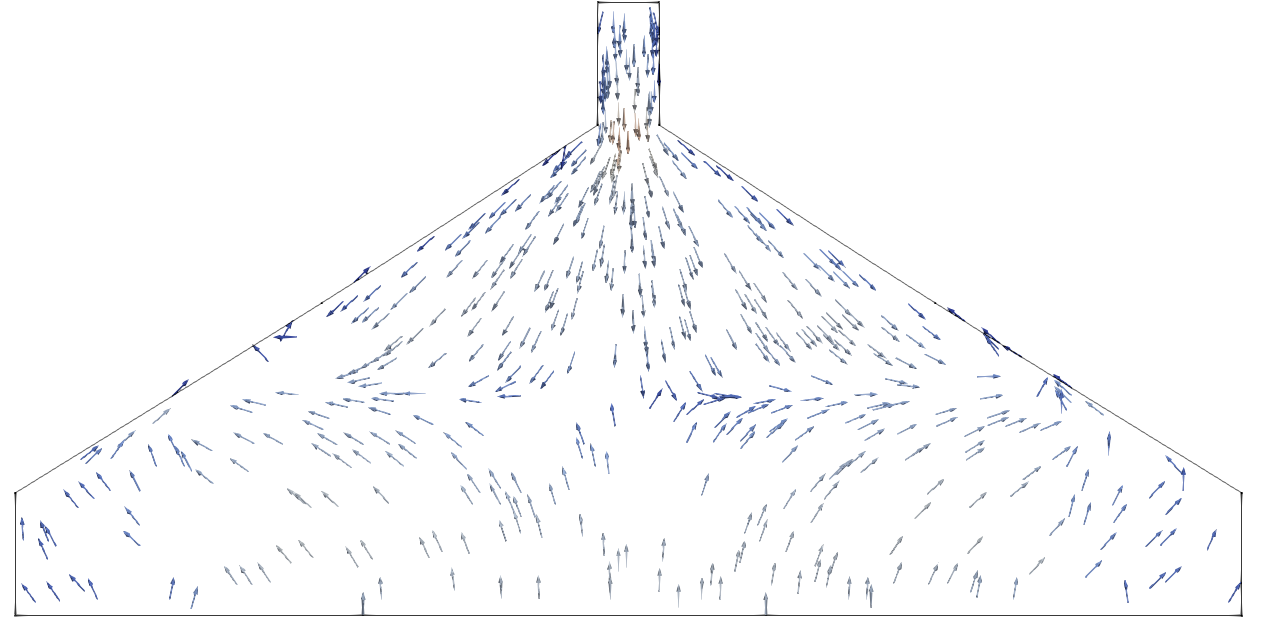
\includegraphics[width=0.96\textwidth]{velocity_field_case_4_trapezoidal_04_20.png}
        \subcaption{}
    \end{subfigure}
    \begin{subfigure}[b]{0.44\textwidth}
        \centering
        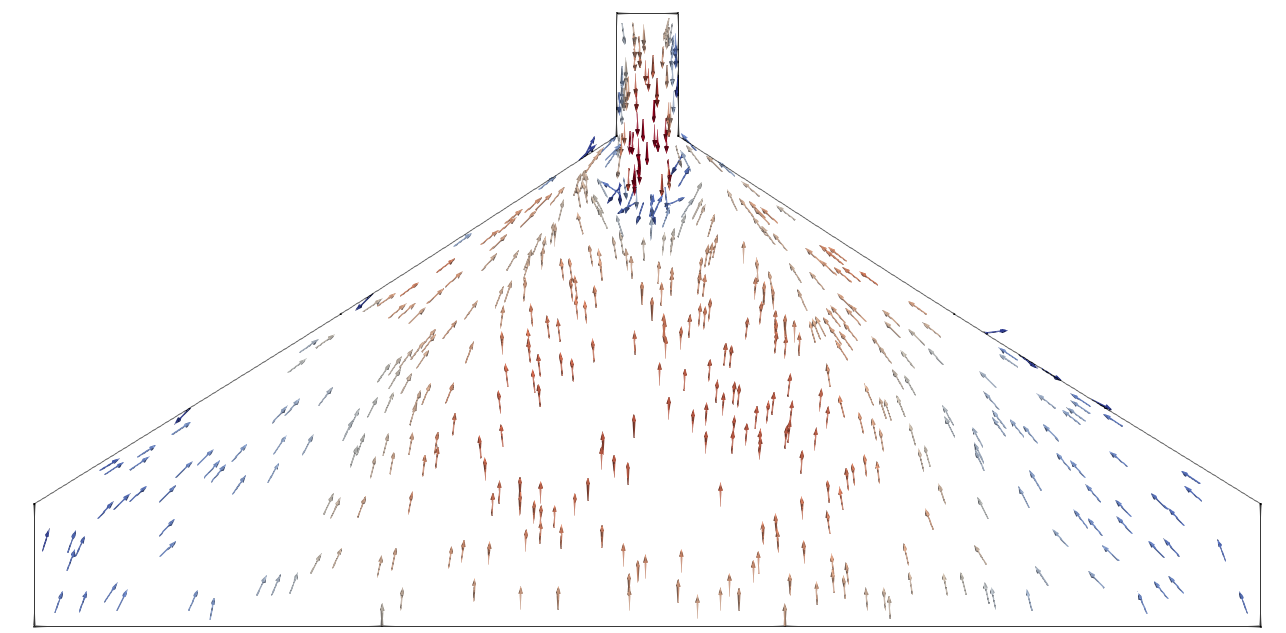
\includegraphics[width=0.96\textwidth]{velocity_field_case_4_trapezoidal_08_20.png}
        \subcaption{}
    \end{subfigure}
    \begin{subfigure}[b]{0.10\textwidth}
        \centering
        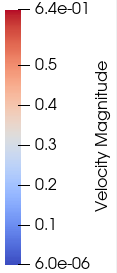
\includegraphics[width=0.96\textwidth]{velocity_field_case_4_trapezoidal_axis.png}
        \vspace{1.0pt}
    \end{subfigure}
    \\
    \begin{subfigure}[b]{0.44\textwidth}
        \centering
        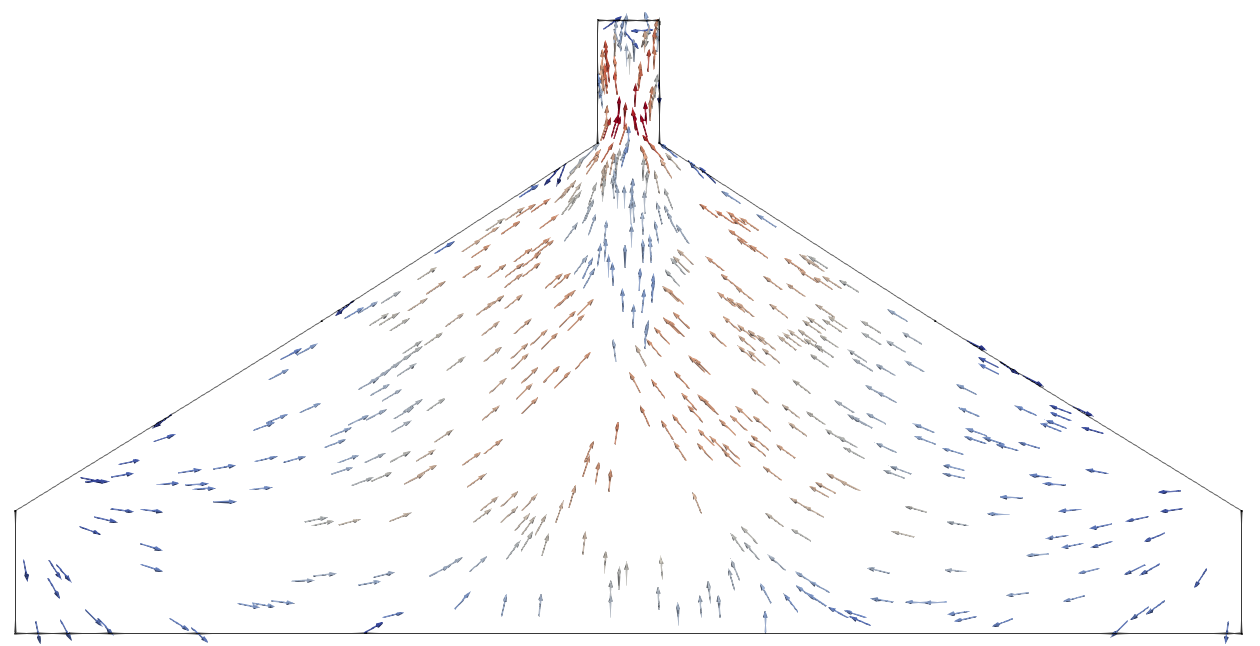
\includegraphics[width=0.96\textwidth]{velocity_field_case_4_trapezoidal_11_20.png}
        \subcaption{}
    \end{subfigure}
    \begin{subfigure}[b]{0.44\textwidth}
        \centering
        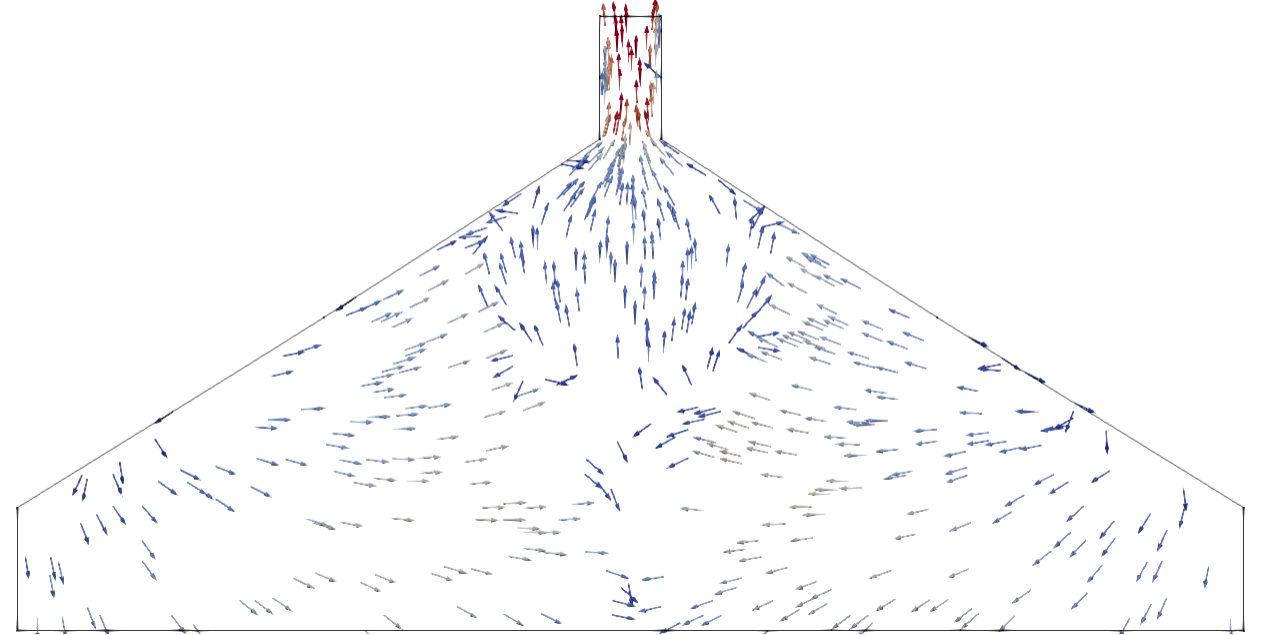
\includegraphics[width=0.96\textwidth]{velocity_field_case_4_trapezoidal_13_20.png}
        \subcaption{}
    \end{subfigure}
    \captionsetup{font=scriptsize}
    \caption{
    Velocity vector diagrams at 4 time points (a:$\frac{4}{20}T$,b:$\frac{8}{20}T$,c:$\frac{11}{20}T$,d:$\frac{13}{20}T$) during the ``upward push half-cycle'' for the trapezoidal shape chamber under Case 4.
    Supports stronger fluid collisions in ejection phase.
    }
    \label{fig:velocity_field_case_4_trapezoidal}
\end{figure}

\begin{figure}[htbp]
    %\centering
    \begin{subfigure}[b]{0.44\textwidth}
        \centering
        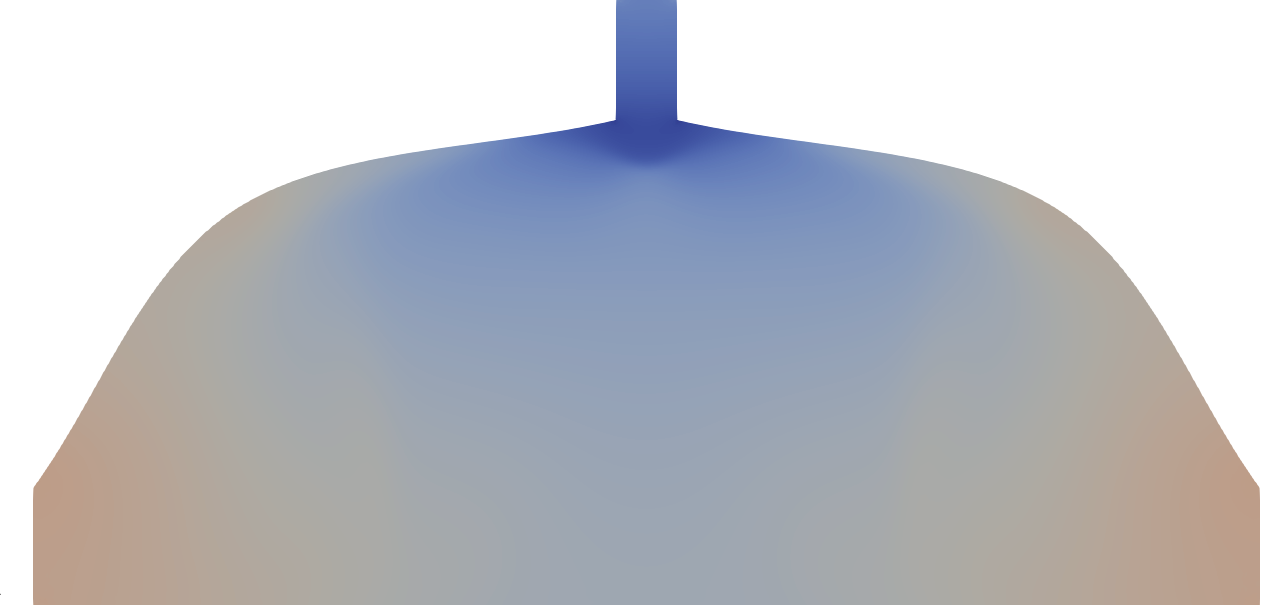
\includegraphics[width=0.96\textwidth]{pressure_field_case_4_arched_08_20.png}
        \subcaption{}
    \end{subfigure}
    \begin{subfigure}[b]{0.44\textwidth}
        \centering
        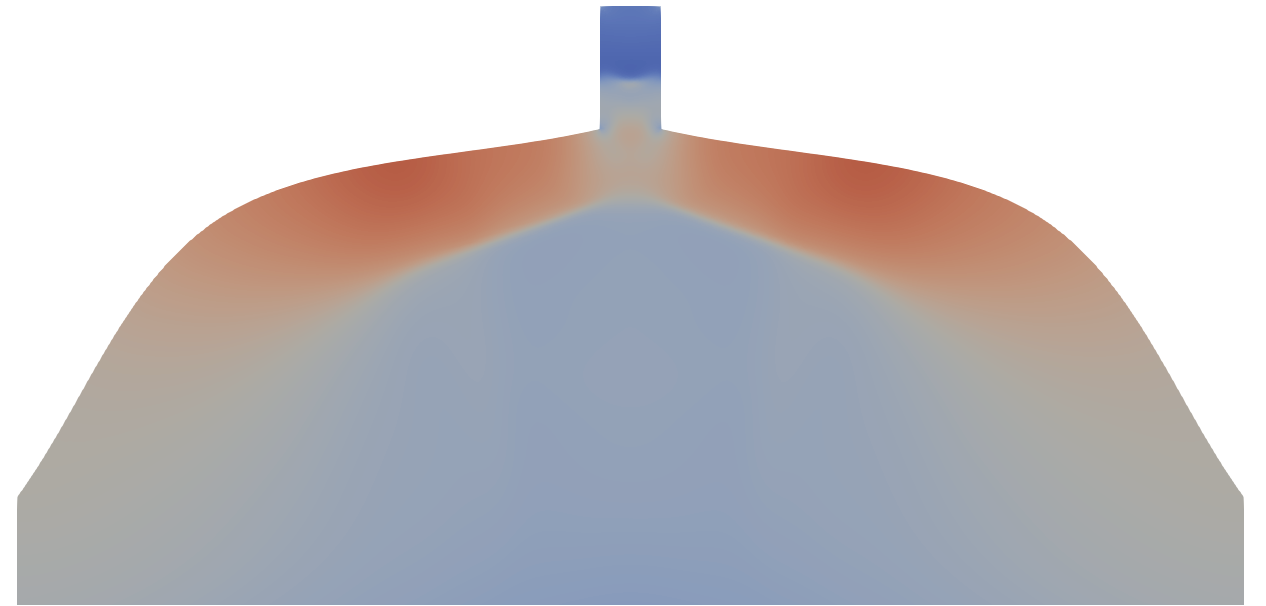
\includegraphics[width=0.96\textwidth]{pressure_field_case_4_arched_10_20.png}
        \subcaption{}
    \end{subfigure}
    \begin{subfigure}[b]{0.10\textwidth}
        \centering
        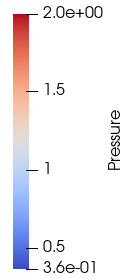
\includegraphics[width=0.96\textwidth]{pressure_field_case_4_arched_axis.png}
        \vspace{1.0pt}
    \end{subfigure}
    \\
    \begin{subfigure}[b]{0.44\textwidth}
        \centering
        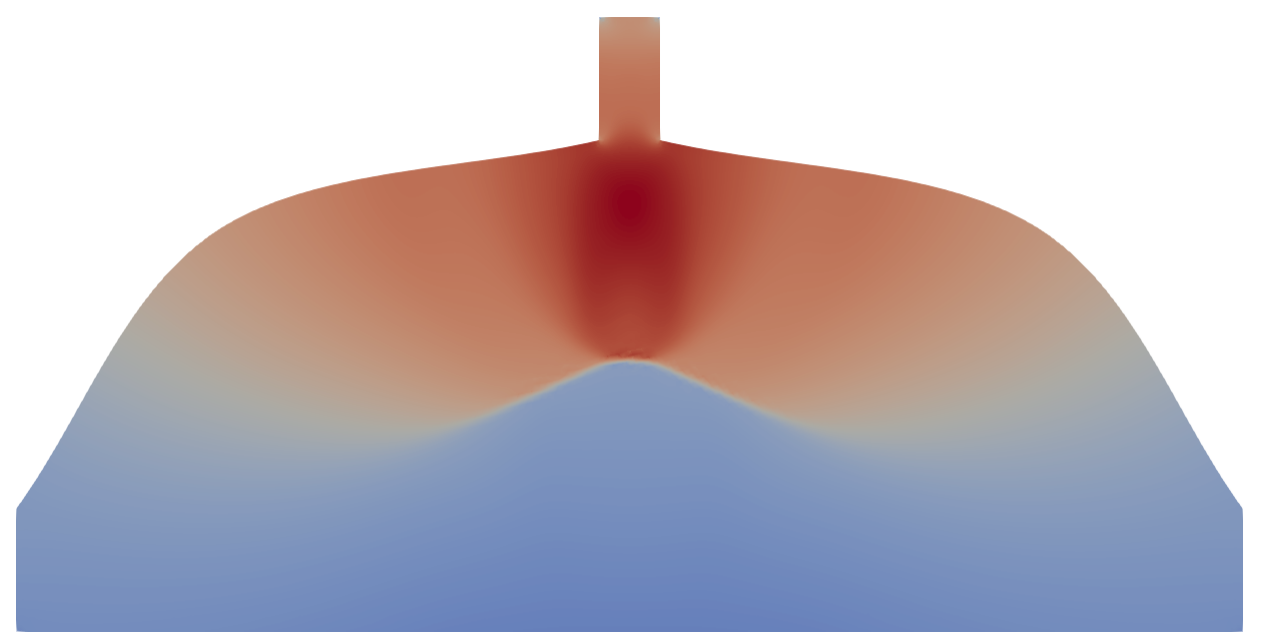
\includegraphics[width=0.96\textwidth]{pressure_field_case_4_arched_13_20.png}
        \subcaption{}
    \end{subfigure}
    \begin{subfigure}[b]{0.44\textwidth}
        \centering
        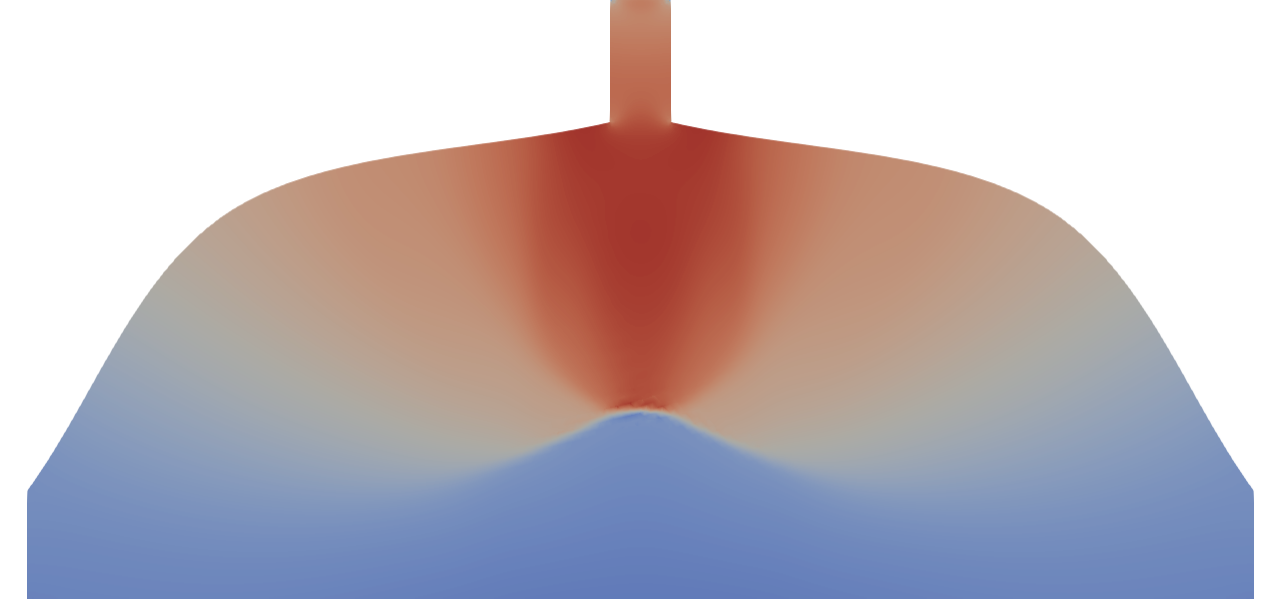
\includegraphics[width=0.96\textwidth]{pressure_field_case_4_arched_14_20.png}
        \subcaption{}
    \end{subfigure}
    \captionsetup{font=scriptsize}
    \caption{
    Pressure contours at 4 time points (a:$\frac{8}{20}T$,b:$\frac{10}{20}T$,c:$\frac{13}{20}T$,d:$\frac{14}{20}T$) during the ``upward push half-cycle'' for the arched chamber under Case 4.
    Upper part disperses pressure (b) and alleviates pressure wave divergence (c)(d).
    }
    \label{fig:pressure_field_case_4_arched}
\end{figure}

\begin{figure}[htbp]
    %\centering
    \begin{subfigure}[b]{0.44\textwidth}
        \centering
        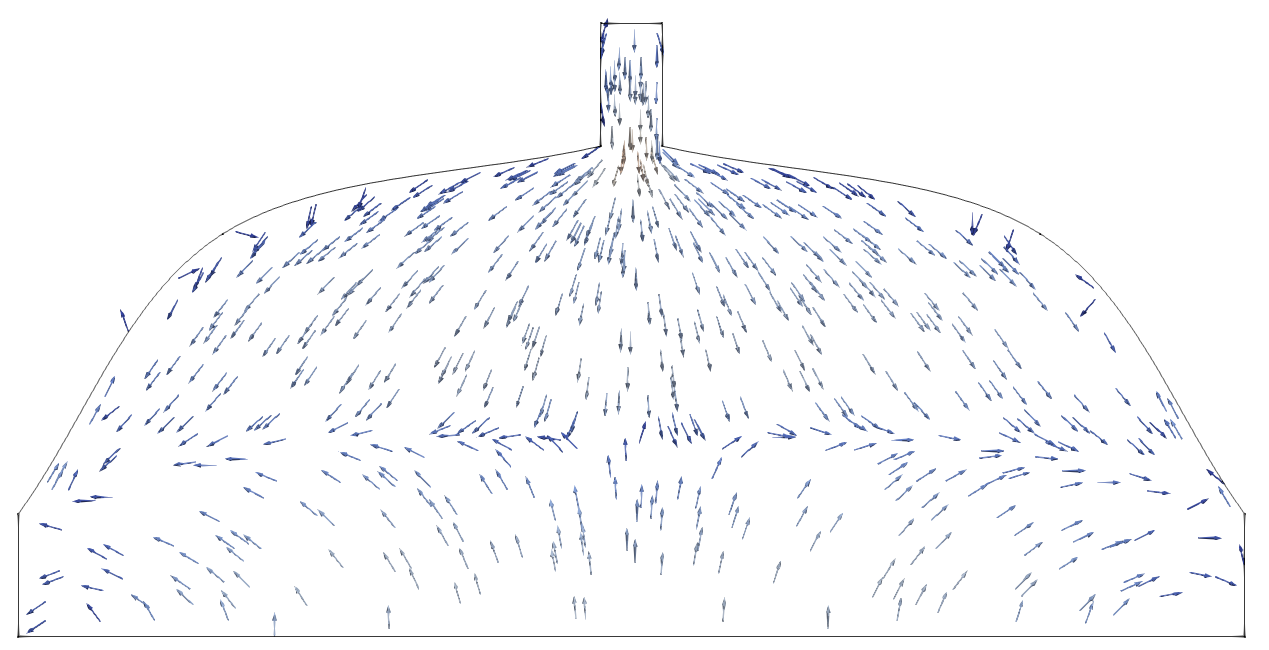
\includegraphics[width=0.96\textwidth]{velocity_field_case_4_arched_04_20.png}
        \subcaption{}
    \end{subfigure}
    \begin{subfigure}[b]{0.44\textwidth}
        \centering
        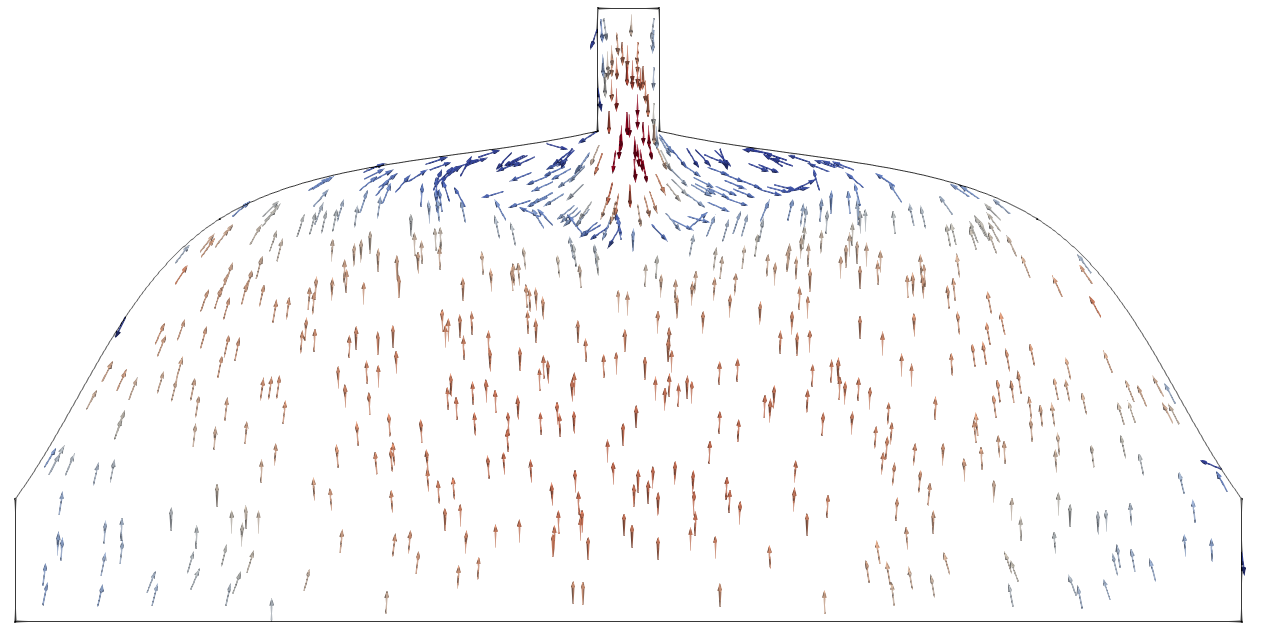
\includegraphics[width=0.96\textwidth]{velocity_field_case_4_arched_07_20.png}
        \subcaption{}
    \end{subfigure}
    \begin{subfigure}[b]{0.10\textwidth}
        \centering
        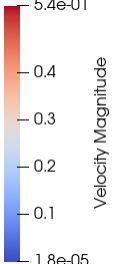
\includegraphics[width=0.96\textwidth]{velocity_field_case_4_arched_axis.png}
        \vspace{1.0pt}
    \end{subfigure}
    \\
    \begin{subfigure}[b]{0.44\textwidth}
        \centering
        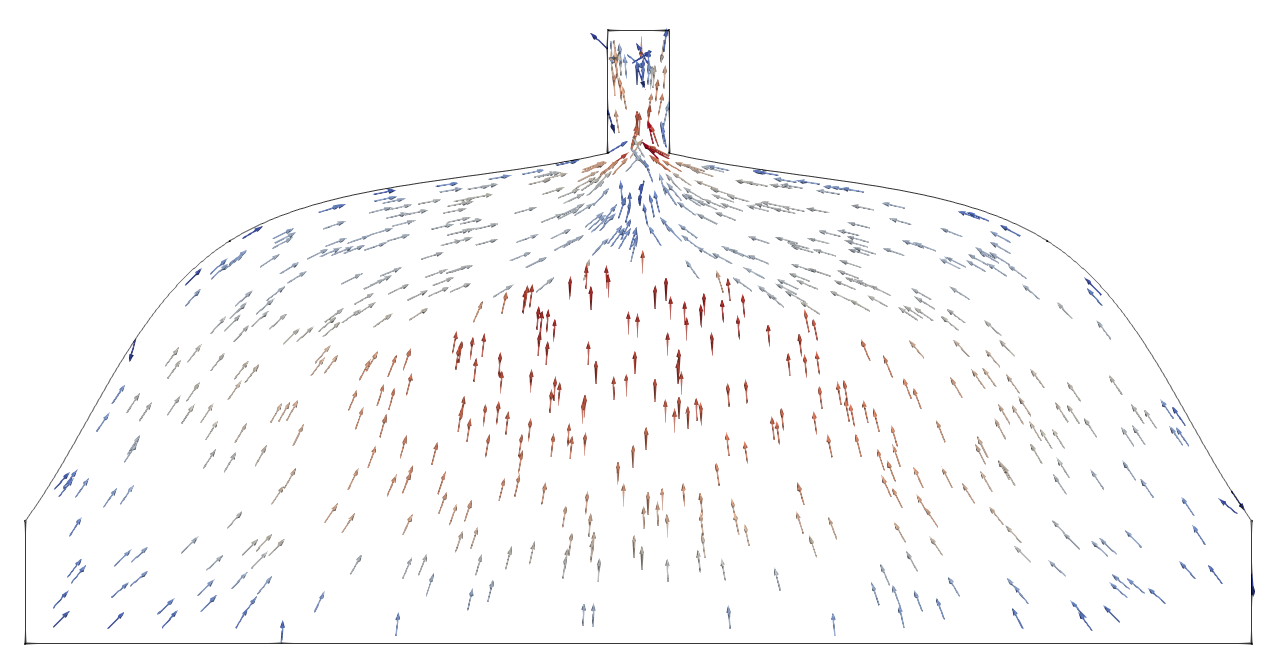
\includegraphics[width=0.96\textwidth]{velocity_field_case_4_arched_11_20.png}
        \subcaption{}
    \end{subfigure}
    \begin{subfigure}[b]{0.44\textwidth}
        \centering
        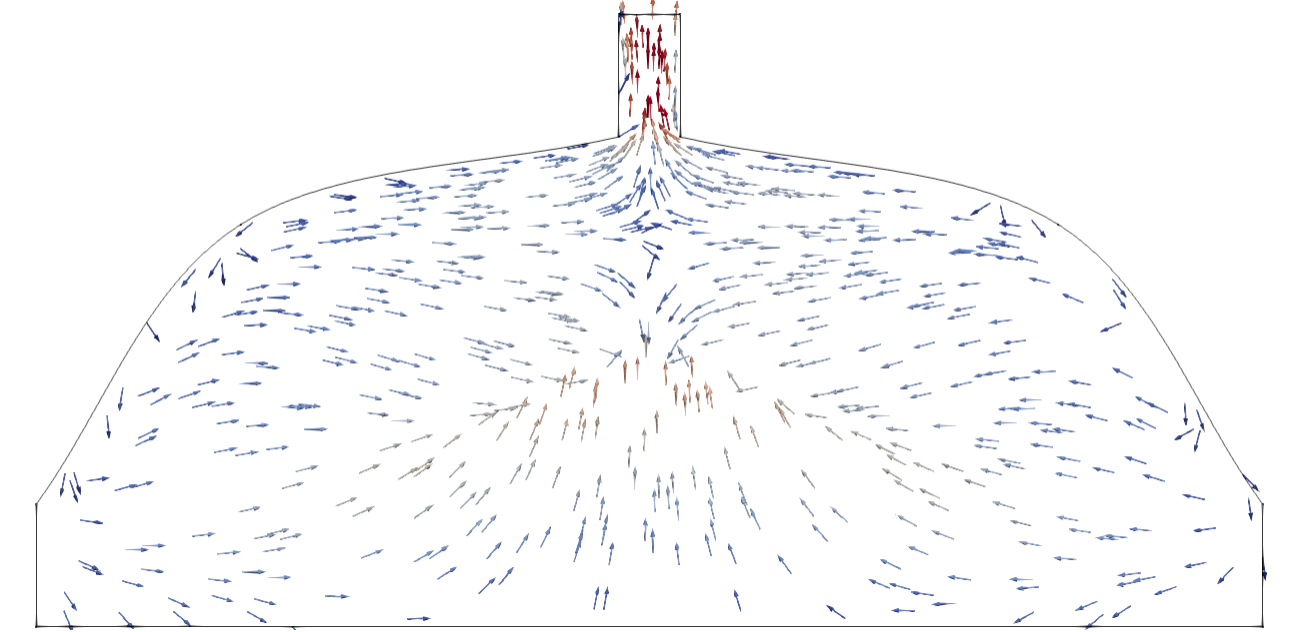
\includegraphics[width=0.96\textwidth]{velocity_field_case_4_arched_13_20.png}
        \subcaption{}
    \end{subfigure}
    \captionsetup{font=scriptsize}
    \caption{
    Velocity vector diagrams at 4 time points (a:$\frac{4}{20}T$,b:$\frac{7}{20}T$,c:$\frac{11}{20}T$,d:$\frac{13}{20}T$) during the ``upward push half-cycle'' for the arched shape chamber under Case 4.
    Despite ``center-on collision'' (c)(d), outlet velocity loss is not large.
    }
    \label{fig:velocity_field_case_4_arched}
\end{figure}

Compared to Case 0, fluid motion in Case 4 (trapezoidal/arched) is similar but significantly more violent.
Upward pushing and pressure ``diffusion'' along walls are faster.
Especially in ejection phase, higher speeds lead to stronger collisions and pressure waves diverging from the center (Figure \ref{fig:pressure_field_case_4_trapezoidal}, Figure \ref{fig:pressure_field_case_4_arched}), which is shows obviously in the pressure contour.
Divergence is visually obvious in Case 4 but not Case 0.

Analysis of Case 0 pointed out: near-horizontal upper part of arched chamber disperses pressure and enhances ejection collisions.
This qualitative description remains valid for Case 4.
Considering pressure wave divergence, the positive effect of arched chambers in dispersing pressure and alleviating divergence on walls outweighs the negative effect on outlet velocity amplitude.

Case 6 only doubles frequency. Obtained shapes cannot be simply classified as ``inverted T'' or ``S'' (Figure \ref{fig:target_data_of_optimized_shapes_case_6}).

\begin{figure}[htbp]
    \centering
    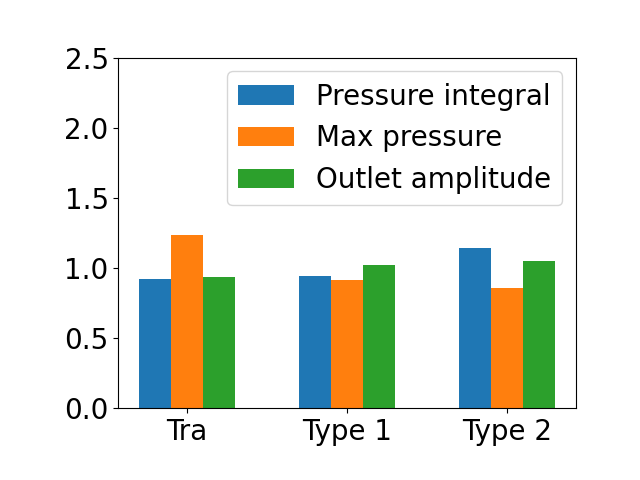
\includegraphics[width=0.64\textwidth]{target_data_case_6.png}
    \captionsetup{font=scriptsize}
    \caption{
    Target data for optimized shapes under Case 6.
    At higher frequency, optimized shapes aren't ``inverted T'' or ``S'', showing more obvious advantages over trapezoidal.
    }
    \label{fig:target_data_of_optimized_shapes_case_6}
\end{figure}

Optimized shapes significantly reduce max pressure while maintaining outlet velocity.
Flow in Case 6 differs significantly from Cases 0-5. Full cycle pressure/velocity maps are provided.
Pressure results focus on different wall locations; velocity results focus on interaction between new flow, previous downward flow, and ejection collisions (Figure \ref{fig:pressure_field_case_6_trapezoidal}(c)).
Analysis uses trapezoidal as a comparison.
Case 6 trapezoidal pressure map (Figure \ref{fig:pressure_field_case_6_trapezoidal}), velocity (Figure \ref{fig:velocity_field_case_6_trapezoidal}).
In Case 4, ``pressure wave divergence'' was mentioned: due to high speed, violent collisions don't dissipate quickly, waves spread from center.
In double-frequency Case 6, ejection collisions not only cause wave divergence but also make fluid ``bounce back'' and flow downward along the wall (Figure \ref{fig:pressure_field_case_6_trapezoidal}(a)(b)).

\begin{figure}[htbp]
    %\centering
    \begin{subfigure}[b]{0.44\textwidth}
        \centering
        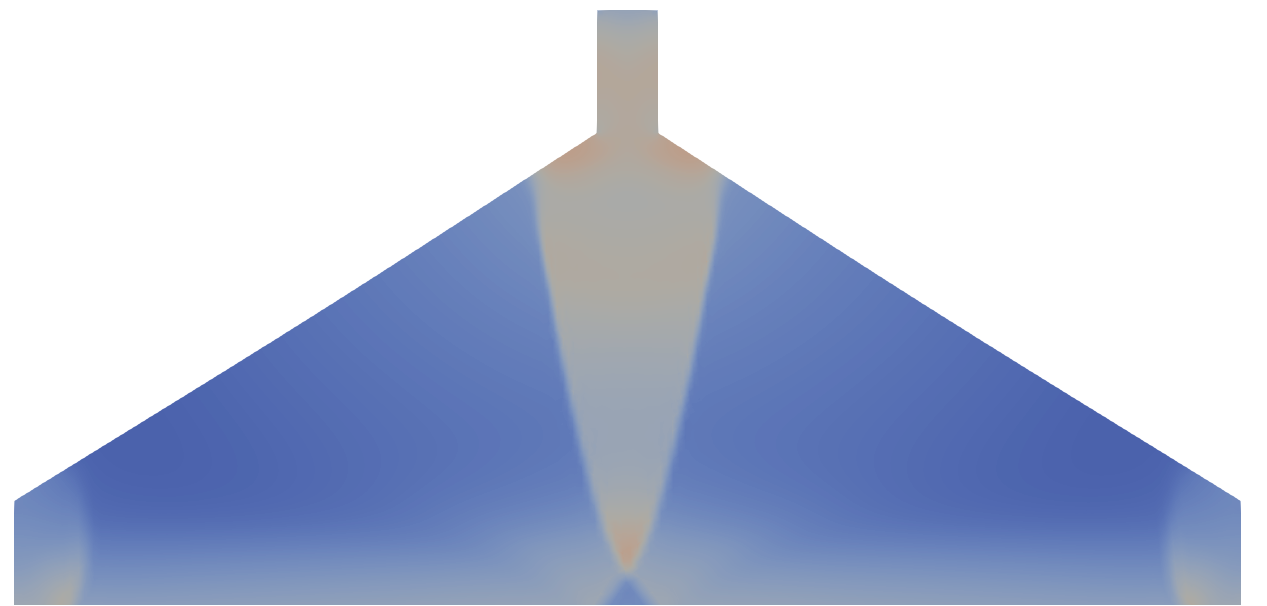
\includegraphics[width=0.96\textwidth]{pressure_field_case_6_trapezoidal_02_10.png}
        \subcaption{}
    \end{subfigure}
    \begin{subfigure}[b]{0.44\textwidth}
        \centering
        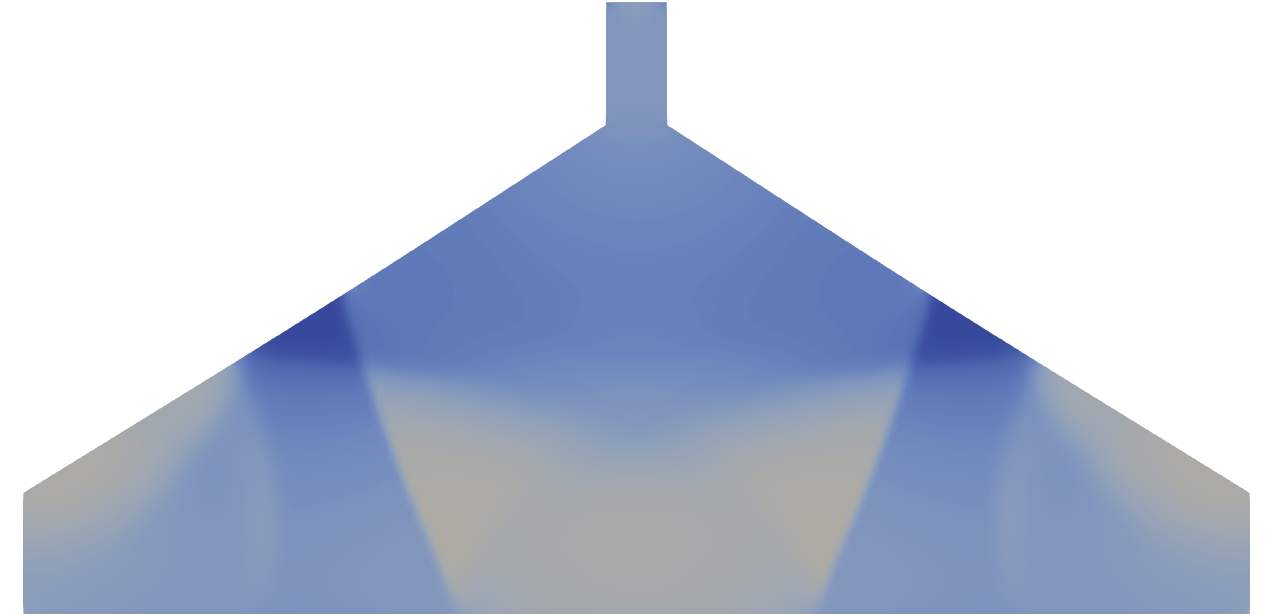
\includegraphics[width=0.96\textwidth]{pressure_field_case_6_trapezoidal_05_10.png}
        \subcaption{}
    \end{subfigure}
    \begin{subfigure}[b]{0.10\textwidth}
        \centering
        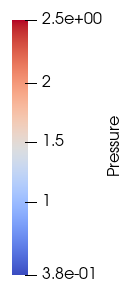
\includegraphics[width=0.96\textwidth]{pressure_field_case_6_trapezoidal_axis.png}
        \vspace{1.0pt}
    \end{subfigure}
    \\
    \begin{subfigure}[b]{0.44\textwidth}
        \centering
        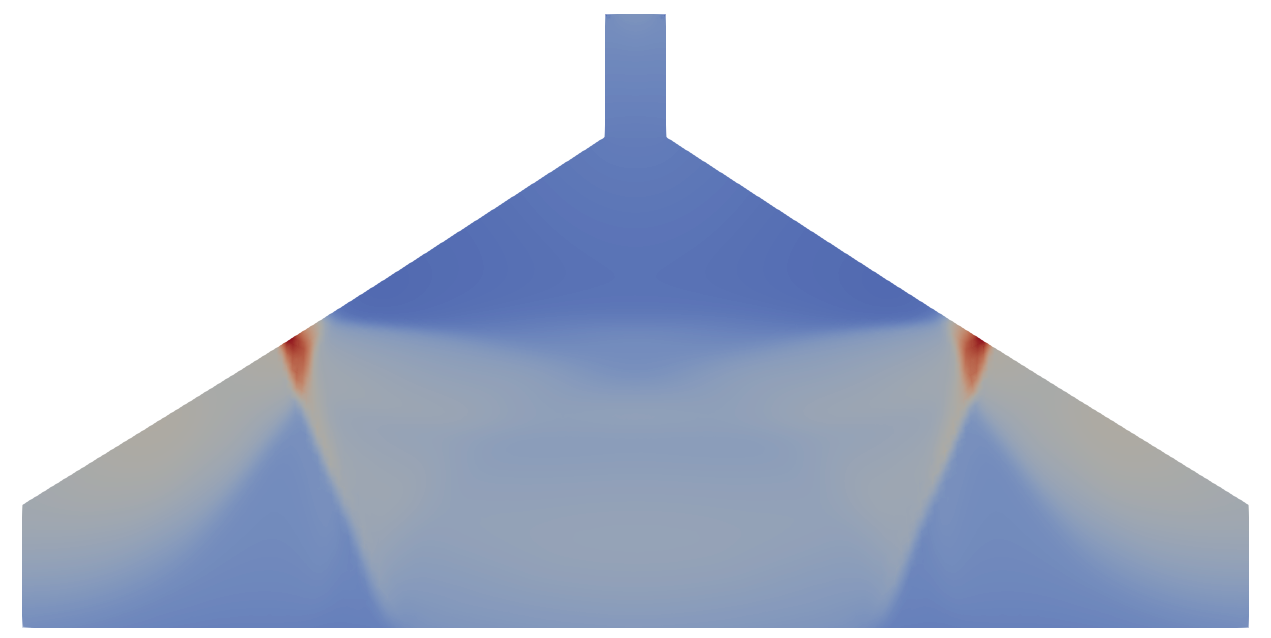
\includegraphics[width=0.96\textwidth]{pressure_field_case_6_trapezoidal_06_10.png}
        \subcaption{}
    \end{subfigure}
    \begin{subfigure}[b]{0.44\textwidth}
        \centering
        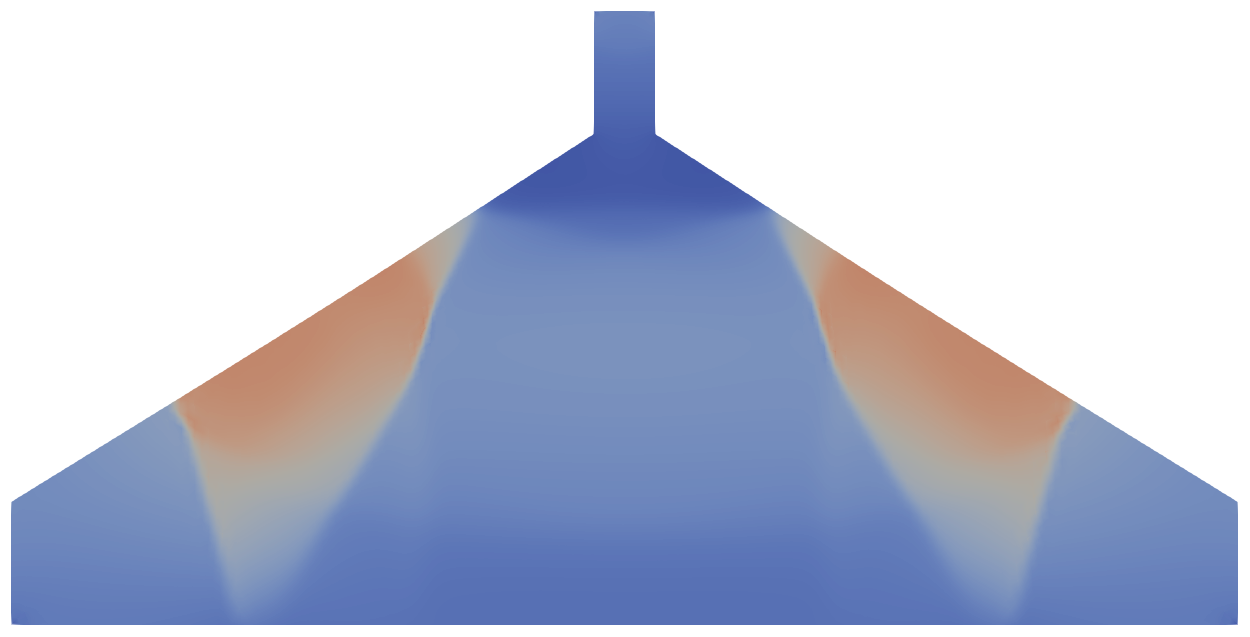
\includegraphics[width=0.96\textwidth]{pressure_field_case_6_trapezoidal_08_10.png}
        \subcaption{}
    \end{subfigure}
    \captionsetup{font=scriptsize}
    \caption{
    Pressure contours at 4 time points (a:$\frac{2}{10}T$,b:$\frac{5}{10}T$,c:$\frac{6}{10}T$,d:$\frac{8}{10}T$) during the ``upward push half-cycle'' for the trapezoidal chamber under Case 6.
    Strong collisions cause bounce back (a)(b); max pressure occurs when downward bounce meets new incoming flow (c).
    }
    \label{fig:pressure_field_case_6_trapezoidal}
\end{figure}

\begin{figure}[htbp]
    %\centering
    \begin{subfigure}[b]{0.44\textwidth}
        \centering
        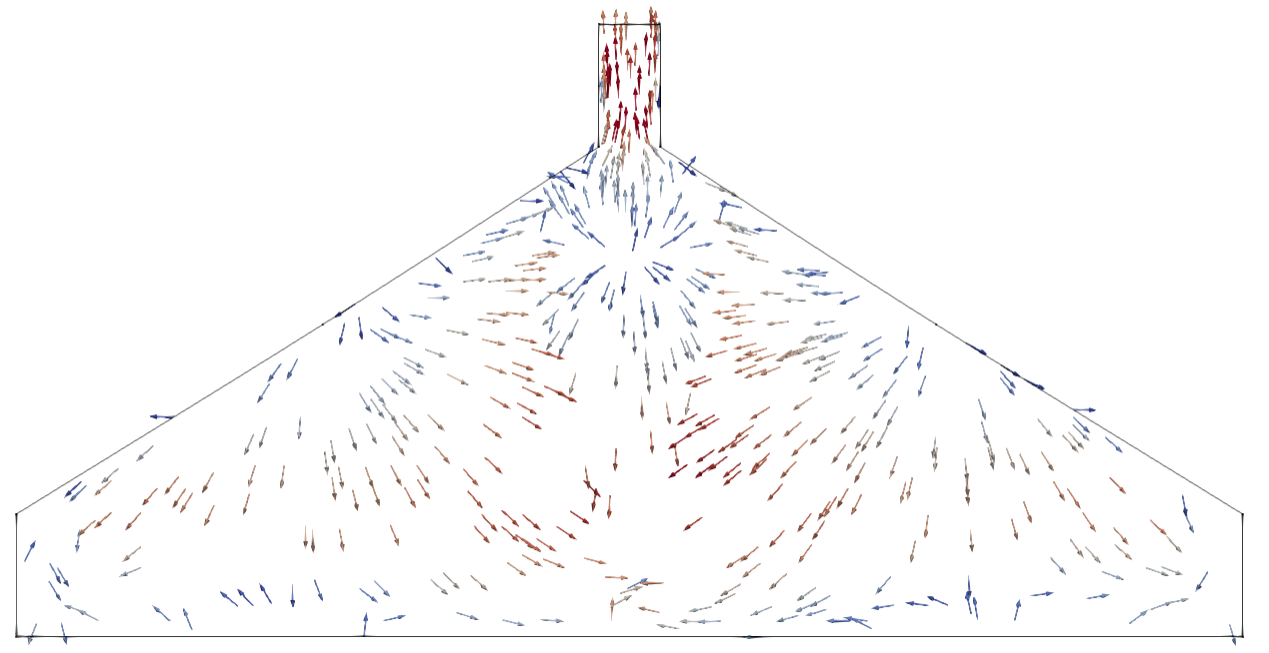
\includegraphics[width=0.96\textwidth]{velocity_field_case_6_trapezoidal_02_10.png}
        \subcaption{}
    \end{subfigure}
    \begin{subfigure}[b]{0.44\textwidth}
        \centering
        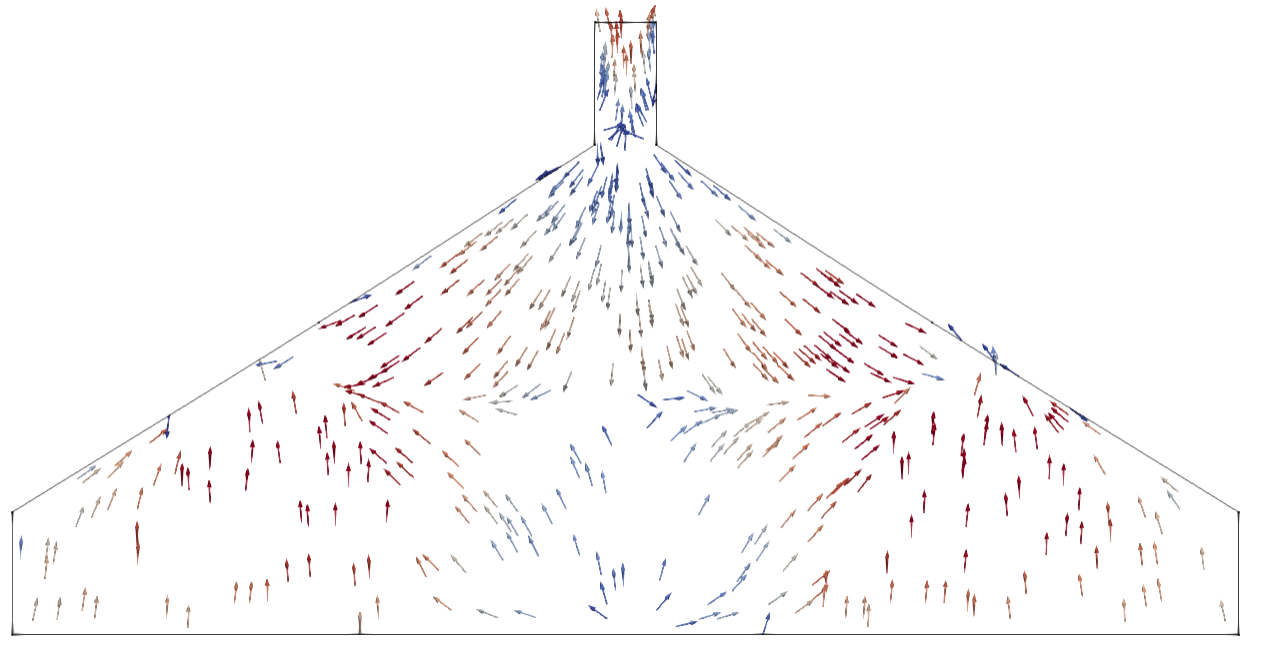
\includegraphics[width=0.96\textwidth]{velocity_field_case_6_trapezoidal_05_10.png}
        \subcaption{}
    \end{subfigure}
    \begin{subfigure}[b]{0.10\textwidth}
        \centering
        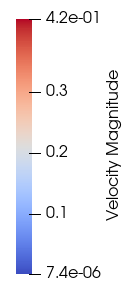
\includegraphics[width=0.96\textwidth]{velocity_field_case_6_trapezoidal_axis.png}
        \vspace{1.0pt}
    \end{subfigure}
    \\
    \begin{subfigure}[b]{0.44\textwidth}
        \centering
        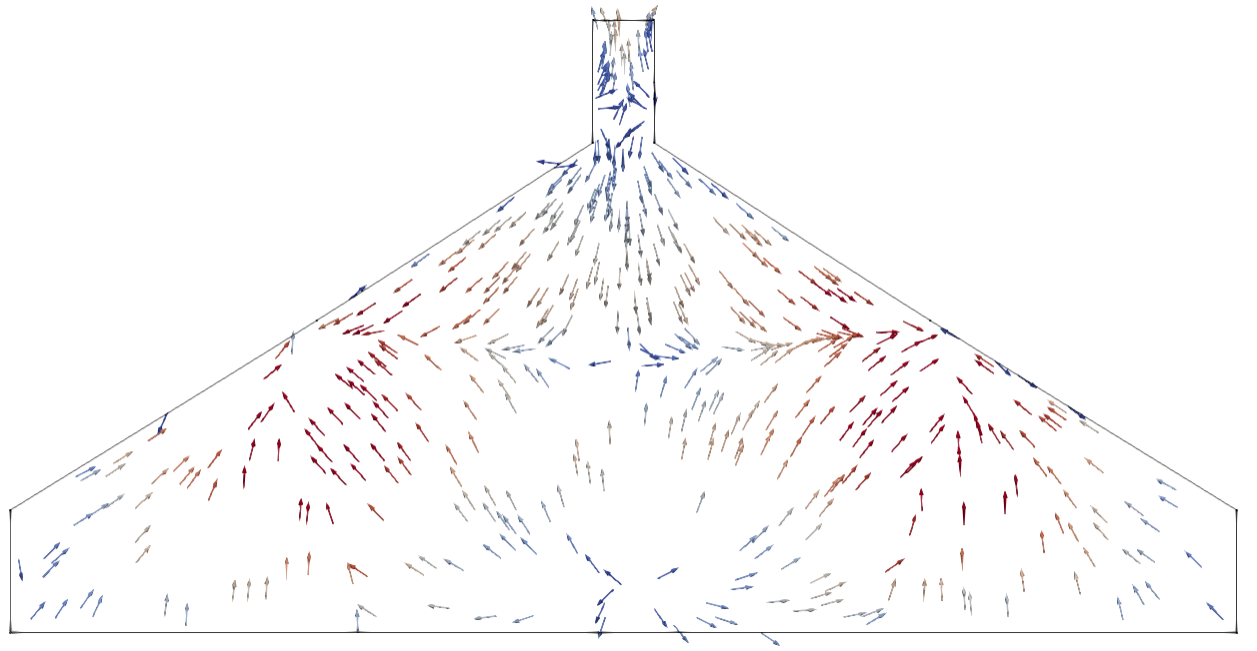
\includegraphics[width=0.96\textwidth]{velocity_field_case_6_trapezoidal_06_10.png}
        \subcaption{}
    \end{subfigure}
    \begin{subfigure}[b]{0.44\textwidth}
        \centering
        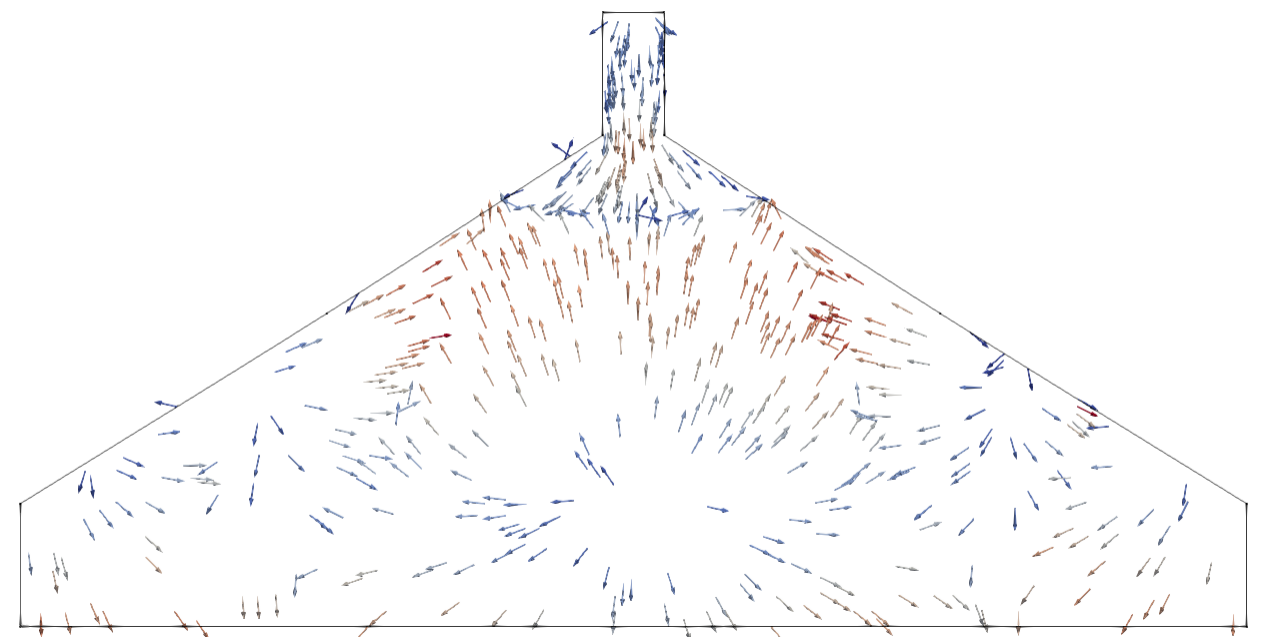
\includegraphics[width=0.96\textwidth]{velocity_field_case_6_trapezoidal_08_10.png}
        \subcaption{}
    \end{subfigure}
    \captionsetup{font=scriptsize}
    \caption{
    Velocity vector diagrams at 4 time points (a:$\frac{2}{10}T$,b:$\frac{5}{10}T$,c:$\frac{6}{10}T$,d:$\frac{8}{10}T$) during the ``upward push half-cycle'' for the trapezoidal shape chamber under Case 6.
    Velocity vectors confirm complex collision and bounce back (a)(c).
    }
    \label{fig:velocity_field_case_6_trapezoidal}
\end{figure}

Observing the four pressure maps (Figure \ref{fig:pressure_field_case_6_trapezoidal}) sequentially:
1. Bounce back from upper center does not dissipate, moves down along wall (Figure \ref{fig:pressure_field_case_6_trapezoidal}(a)(b));
2. Fluid in two bottom corners moves up along wall (Figure \ref{fig:pressure_field_case_6_trapezoidal}(a), caused by previous cycle bounce);
3. These upward/downward motions meet new cycle velocity input in middle, causing violent collision (Figure \ref{fig:pressure_field_case_6_trapezoidal}(c)) and second bounce back (max pressure occurs here).
Second bounce downward meets bottom/next cycle for third bounce upward (corners in (a)).
Velocity vectors (Figure \ref{fig:velocity_field_case_6_trapezoidal}) show these three bounce backs.

Case 6, 1-control-point optimized shape pressure map is shown in Figure \ref{fig:pressure_field_case_6_type_1}, and velocity shown in Figure \ref{fig:velocity_field_case_6_type_1}.

\begin{figure}[htbp]
    %\centering
    \begin{subfigure}[b]{0.44\textwidth}
        \centering
        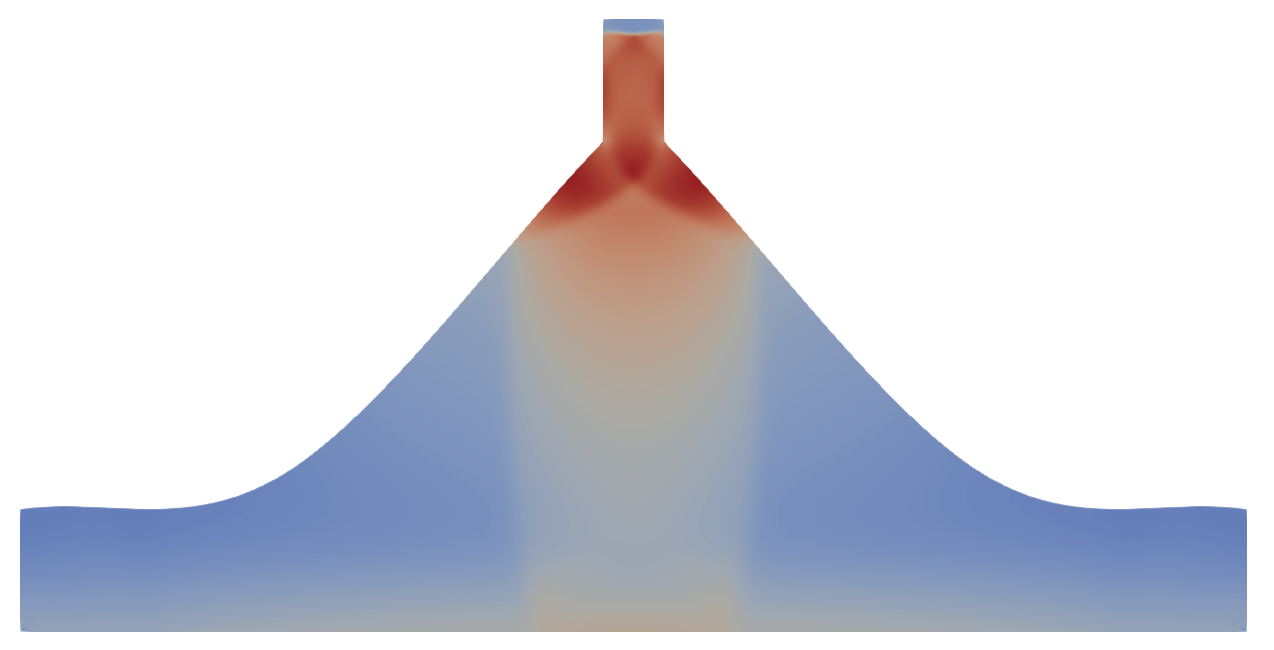
\includegraphics[width=0.96\textwidth]{pressure_field_case_6_type_1_01_10.png}
        \subcaption{}
    \end{subfigure}
    \begin{subfigure}[b]{0.44\textwidth}
        \centering
        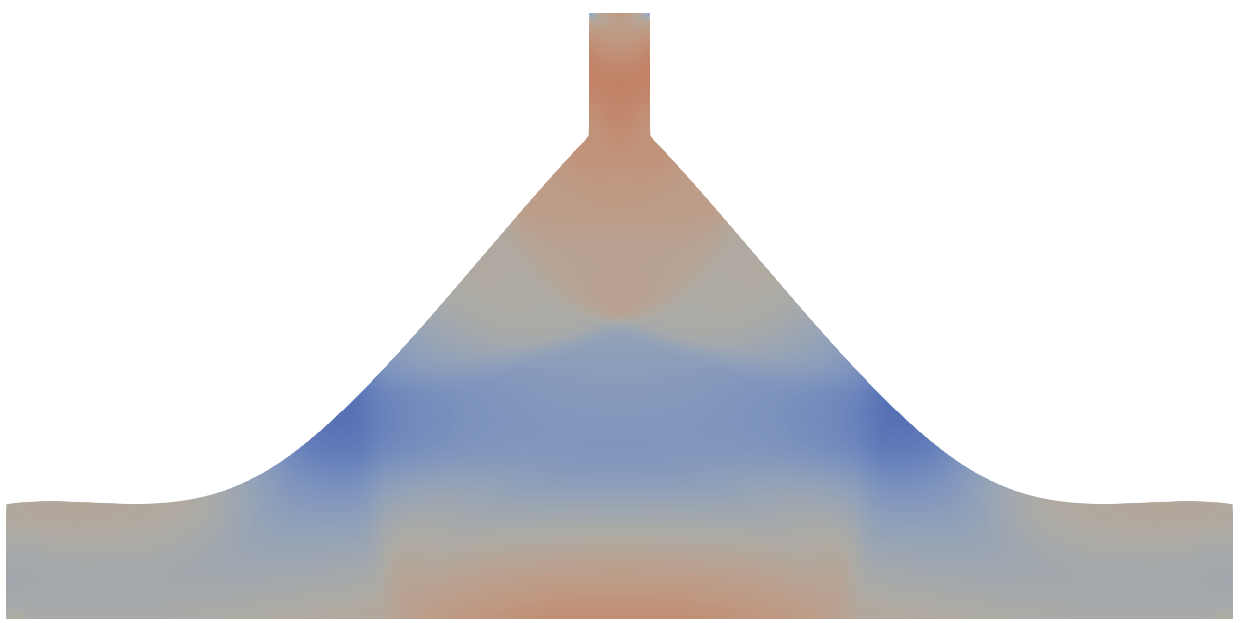
\includegraphics[width=0.96\textwidth]{pressure_field_case_6_type_1_03_10.png}
        \subcaption{}
    \end{subfigure}
    \begin{subfigure}[b]{0.10\textwidth}
        \centering
        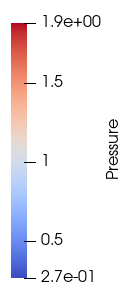
\includegraphics[width=0.96\textwidth]{pressure_field_case_6_type_1_axis.png}
        \vspace{1.0pt}
    \end{subfigure}
    \\
    \begin{subfigure}[b]{0.44\textwidth}
        \centering
        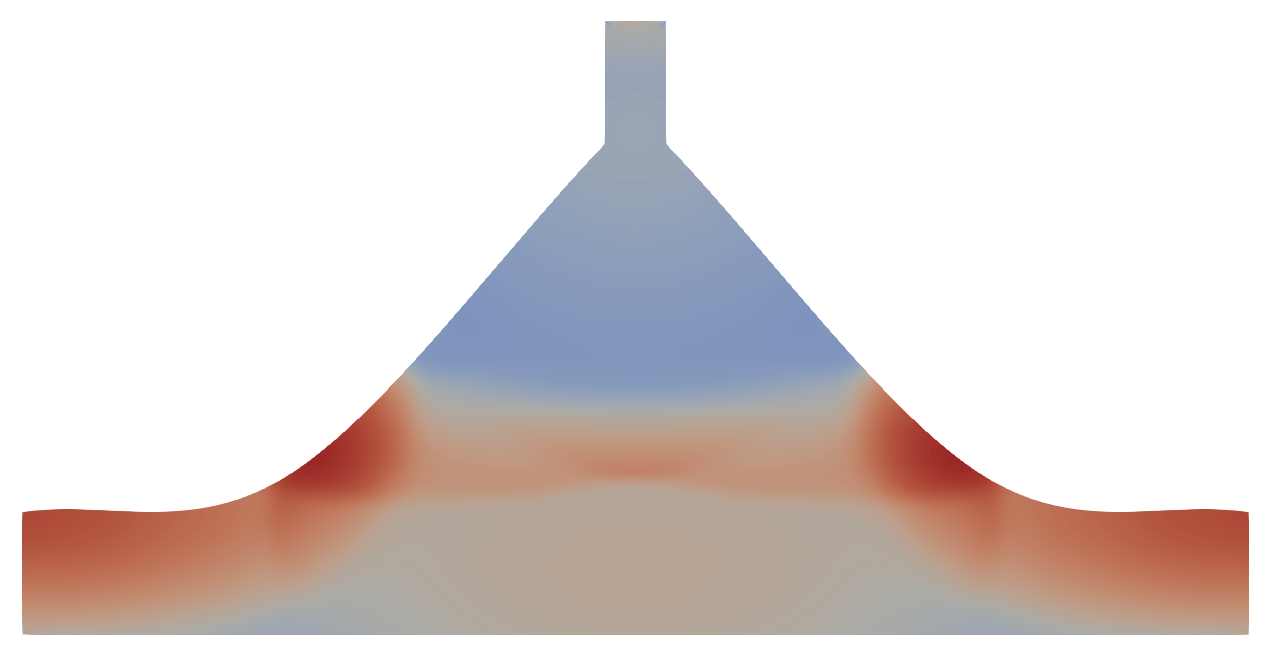
\includegraphics[width=0.96\textwidth]{pressure_field_case_6_type_1_05_10.png}
        \subcaption{}
    \end{subfigure}
    \begin{subfigure}[b]{0.44\textwidth}
        \centering
        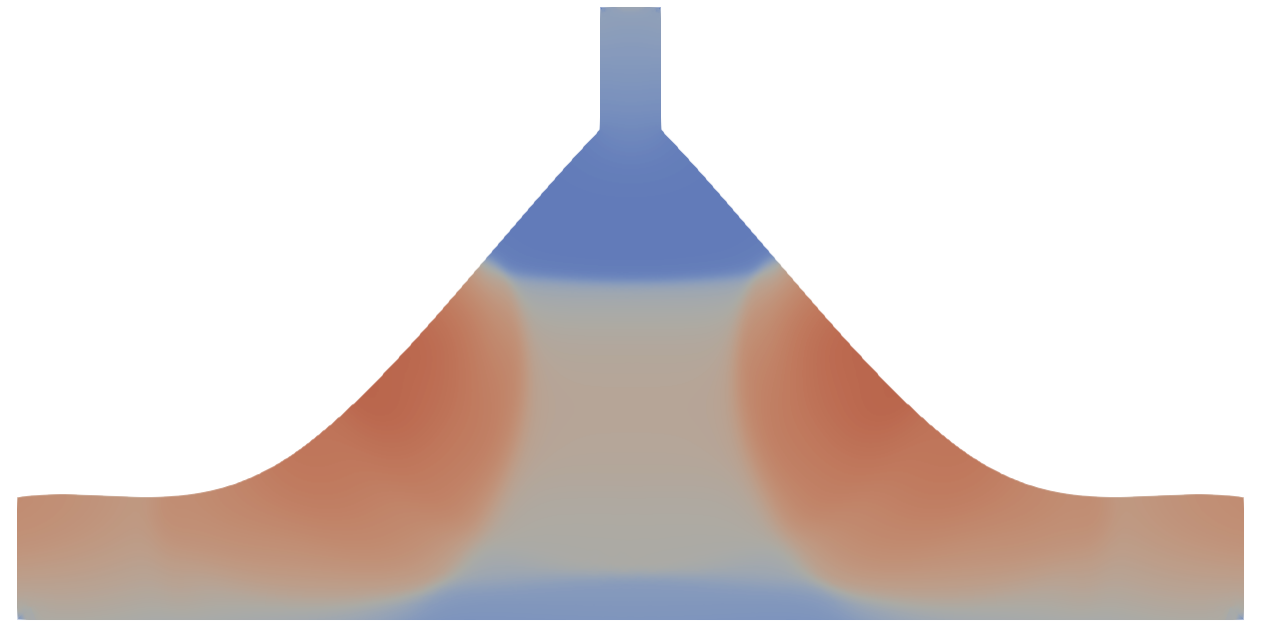
\includegraphics[width=0.96\textwidth]{pressure_field_case_6_type_1_07_10.png}
        \subcaption{}
    \end{subfigure}
    \captionsetup{font=scriptsize}
    \caption{
    Pressure contours at 4 time points (a:$\frac{1}{10}T$,b:$\frac{3}{10}T$,c:$\frac{5}{10}T$,d:$\frac{7}{10}T$) during the ``upward push half-cycle'' for the type 1 chamber under Case 6.
    ``Downward-curving'' shape significantly weakens collision between bounce flow and new incoming flow (c).
    }
    \label{fig:pressure_field_case_6_type_1}
\end{figure}

Compared to trapezoidal, this shape has 3 features:
1. Max pressure also occurs during ejection phase flow toward outlet (Figure \ref{fig:pressure_field_case_6_type_1}(a)) (but lower than trapezoidal),
and it better alleviates collision between downward bounce flow and new incoming flow (Figure \ref{fig:pressure_field_case_6_type_1}(c));
2. Due to ``downward-curving'' wall design, upward corner flows (Figure \ref{fig:pressure_field_case_6_trapezoidal}a) aren't prominent;
only two collisions per cycle: ejection phase (Figure \ref{fig:pressure_field_case_6_type_1}a) and bounce-flow vs new-flow (Figure \ref{fig:pressure_field_case_6_type_1}c);
3. collision between downward bounce flow and new incoming flow occurs exactly at the downward curve (Figure \ref{fig:pressure_field_case_6_type_1}c),
The process changes from ``center-on'' (trapezoidal) to ``eccentric'' collision, significantly reducing intensity.

Thus, the 1-control-point shape reduces bounce backs and lowers intensity of the bounce at the curve.

\begin{figure}[htbp]
    %\centering
    \begin{subfigure}[b]{0.44\textwidth}
        \centering
        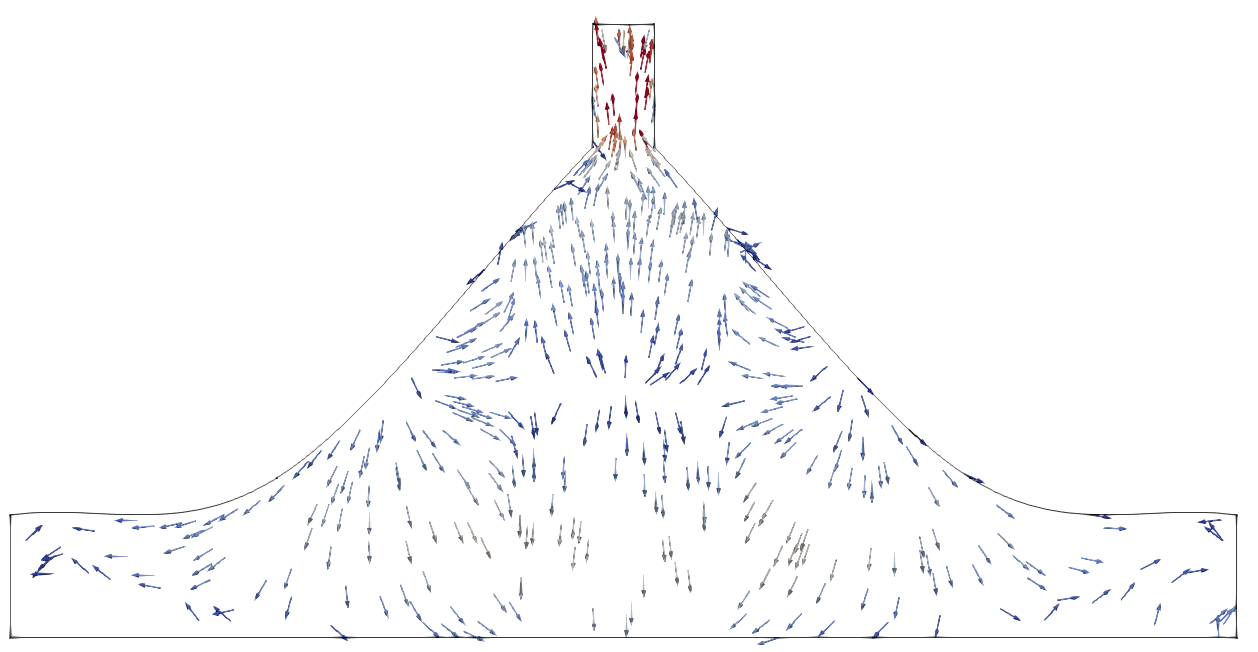
\includegraphics[width=0.96\textwidth]{velocity_field_case_6_type_1_01_10.png}
        \subcaption{}
    \end{subfigure}
    \begin{subfigure}[b]{0.44\textwidth}
        \centering
        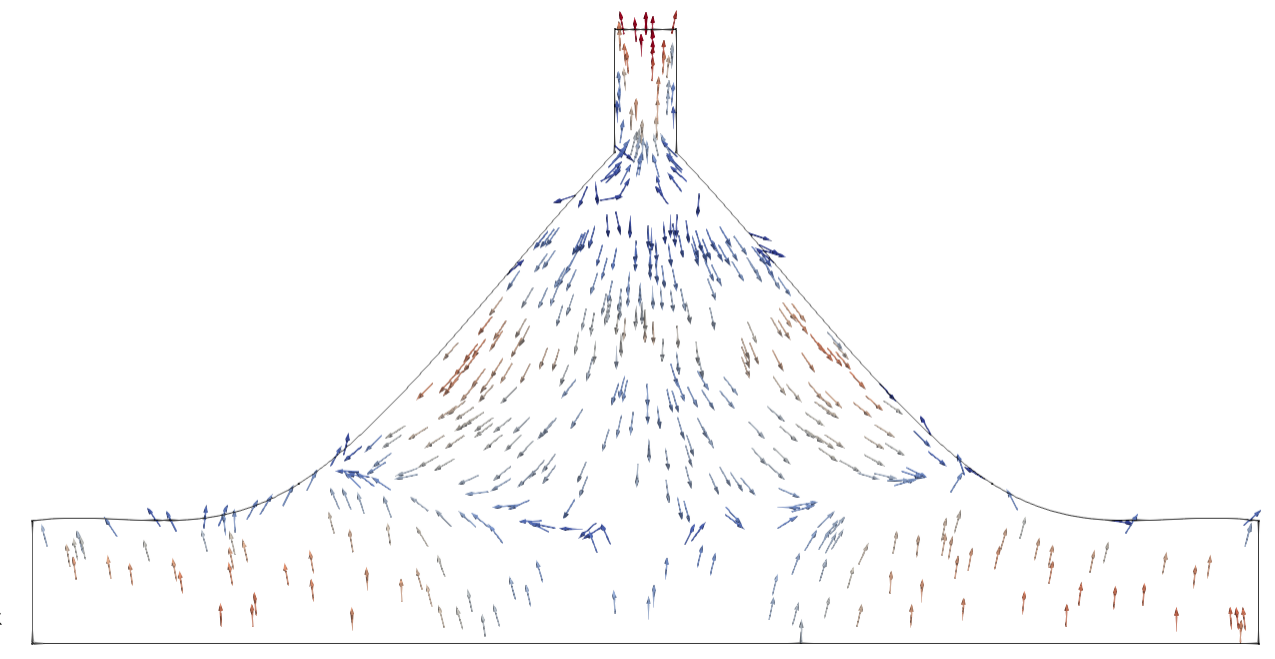
\includegraphics[width=0.96\textwidth]{velocity_field_case_6_type_1_03_10.png}
        \subcaption{}
    \end{subfigure}
    \begin{subfigure}[b]{0.10\textwidth}
        \centering
        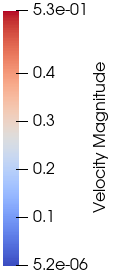
\includegraphics[width=0.96\textwidth]{velocity_field_case_6_type_1_axis.png}
        \vspace{1.0pt}
    \end{subfigure}
    \\
    \begin{subfigure}[b]{0.44\textwidth}
        \centering
        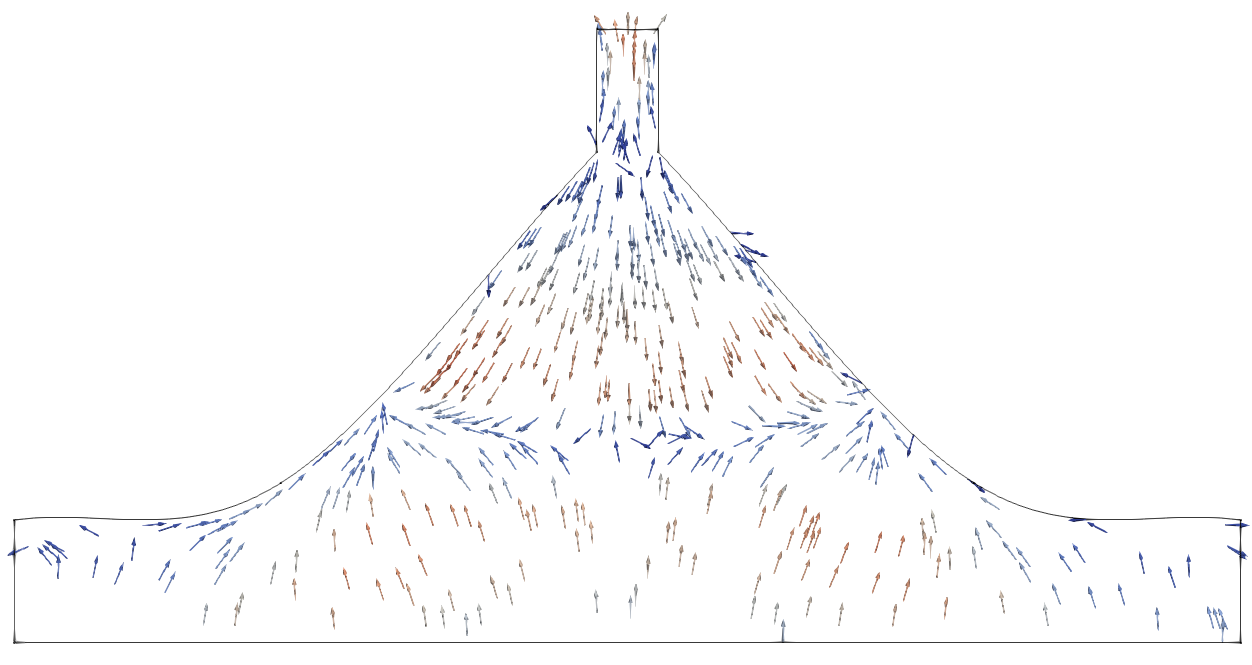
\includegraphics[width=0.96\textwidth]{velocity_field_case_6_type_1_05_10.png}
        \subcaption{}
    \end{subfigure}
    \begin{subfigure}[b]{0.44\textwidth}
        \centering
        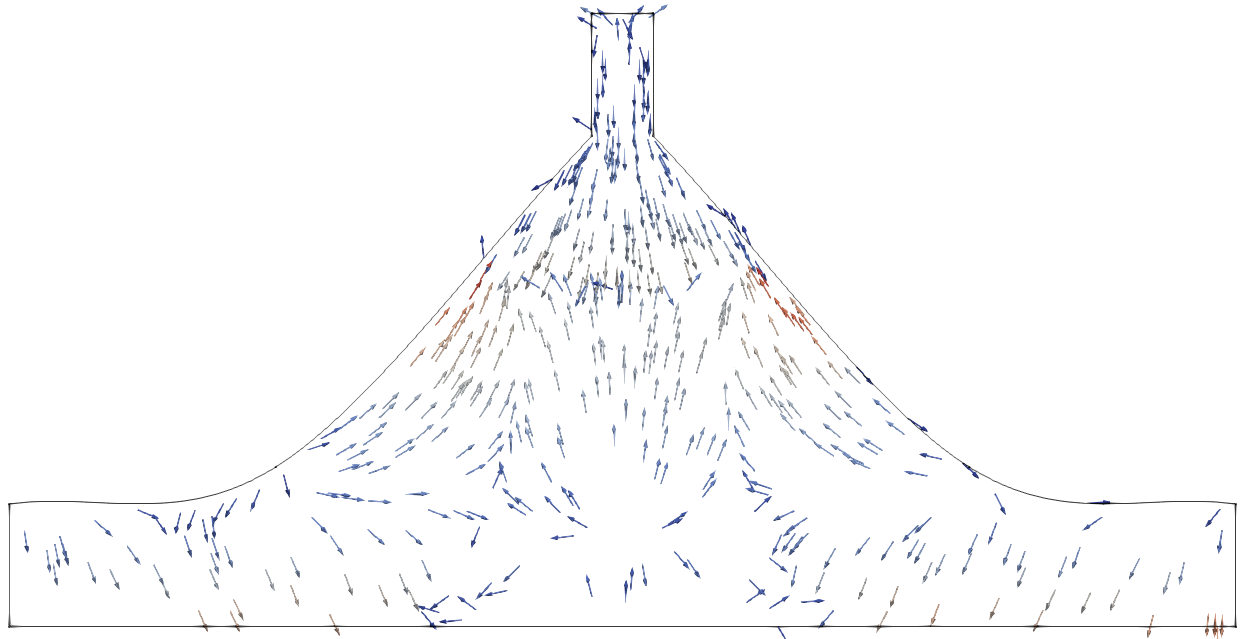
\includegraphics[width=0.96\textwidth]{velocity_field_case_6_type_1_07_10.png}
        \subcaption{}
    \end{subfigure}
    \captionsetup{font=scriptsize}
    \caption{
    Velocity vector diagrams at 4 time points (a:$\frac{1}{10}T$,b:$\frac{3}{10}T$,c:$\frac{5}{10}T$,d:$\frac{7}{10}T$) during the ``upward push half-cycle'' for the type 1 shape chamber under Case 6.
    Shows bounce back (a)(d) and helps explain collision alleviation by ``downward-curving'' shape.
    }
    \label{fig:velocity_field_case_6_type_1}
\end{figure}

Case 6, 2-control-point optimized shape pressure map is shown in Figure \ref{fig:pressure_field_case_6_type_2}, and velocity shown in Figure \ref{fig:velocity_field_case_6_type_2}.

\begin{figure}[htbp]
    %\centering
    \begin{subfigure}[b]{0.44\textwidth}
        \centering
        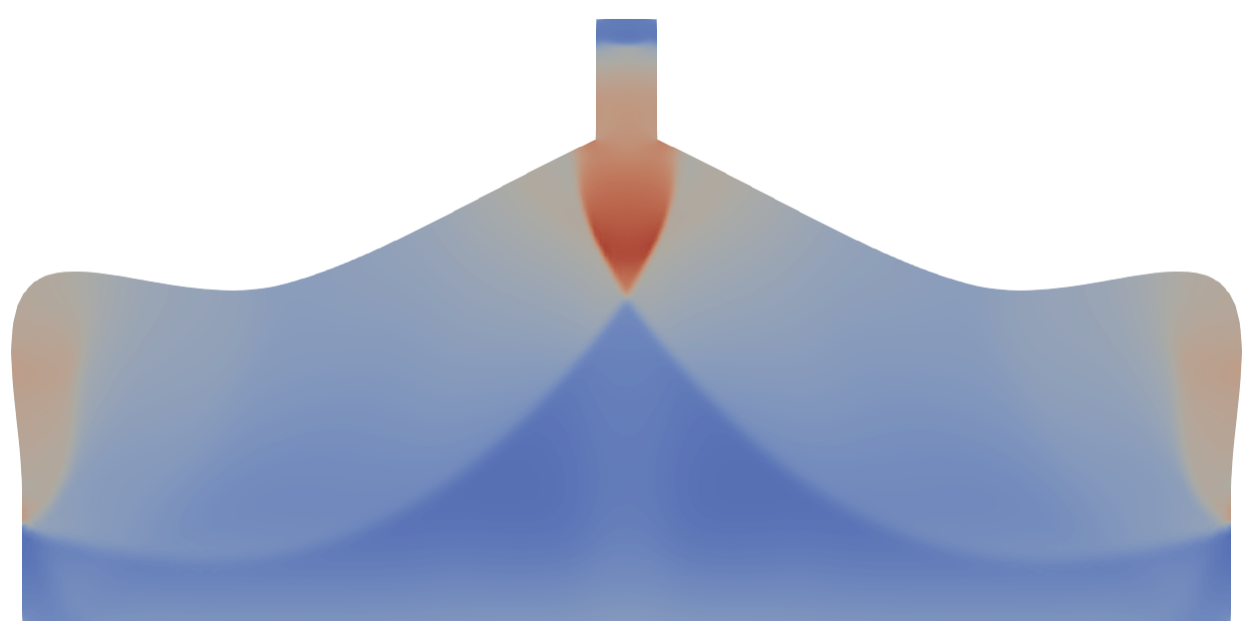
\includegraphics[width=0.96\textwidth]{pressure_field_case_6_type_2_01_10.png}
        \subcaption{}
    \end{subfigure}
    \begin{subfigure}[b]{0.44\textwidth}
        \centering
        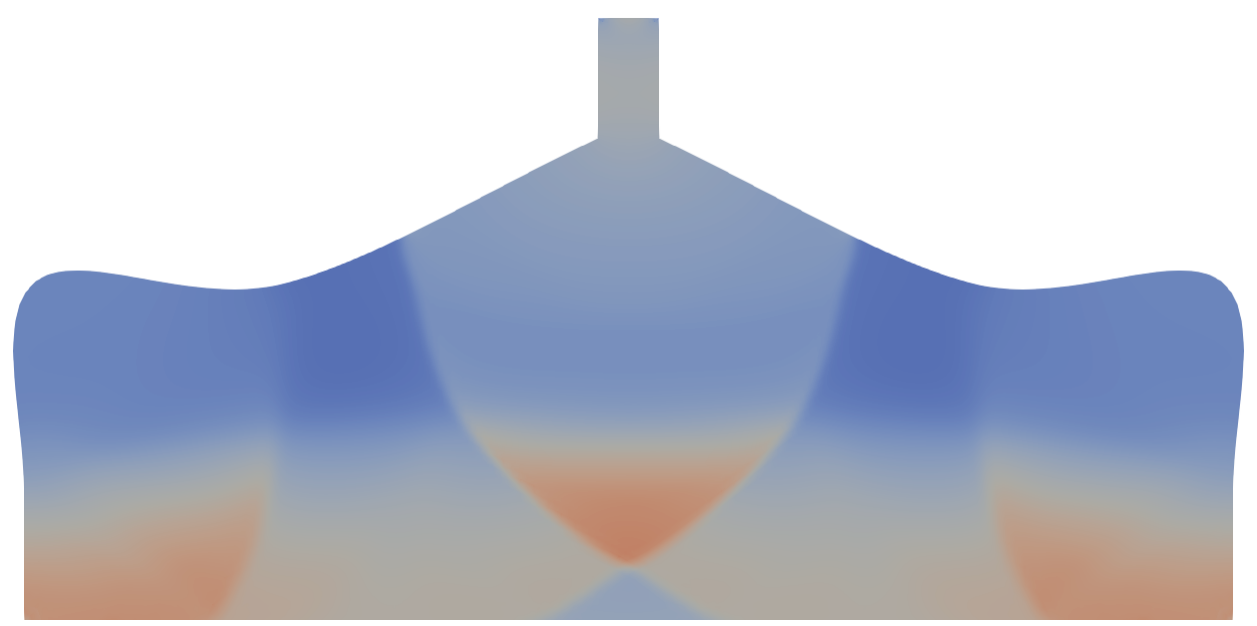
\includegraphics[width=0.96\textwidth]{pressure_field_case_6_type_2_04_10.png}
        \subcaption{}
    \end{subfigure}
    \begin{subfigure}[b]{0.10\textwidth}
        \centering
        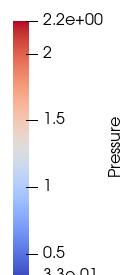
\includegraphics[width=0.96\textwidth]{pressure_field_case_6_type_2_axis.png}
        \vspace{1.0pt}
    \end{subfigure}
    \\
    \begin{subfigure}[b]{0.44\textwidth}
        \centering
        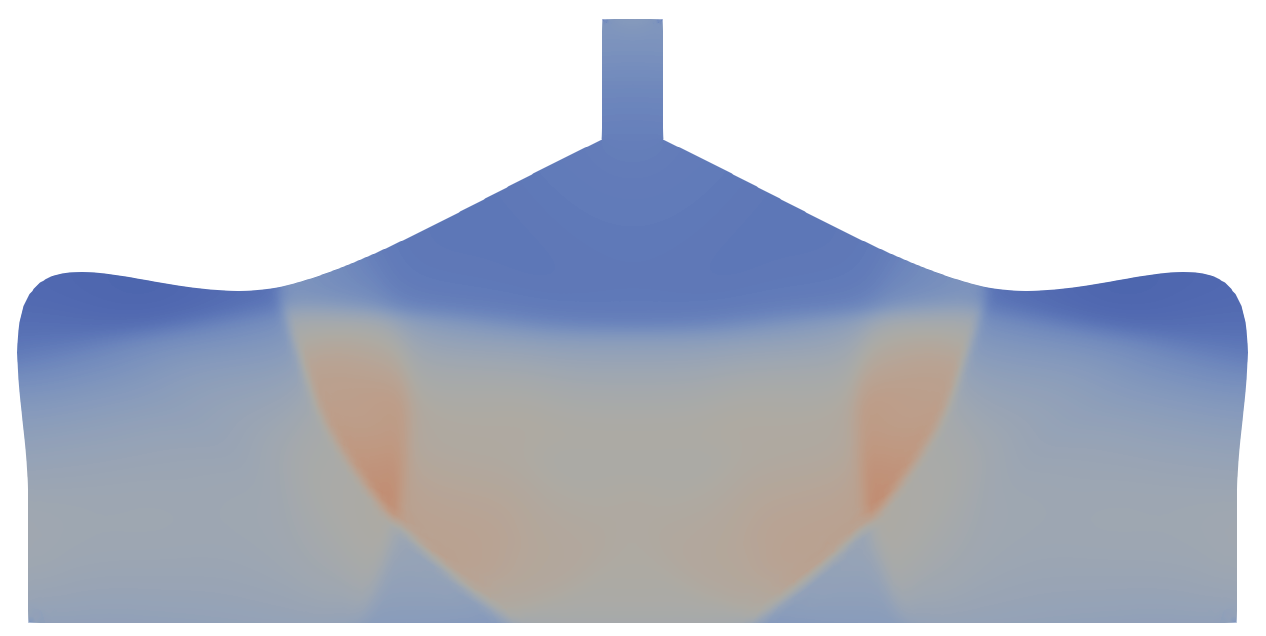
\includegraphics[width=0.96\textwidth]{pressure_field_case_6_type_2_06_10.png}
        \subcaption{}
    \end{subfigure}
    \begin{subfigure}[b]{0.44\textwidth}
        \centering
        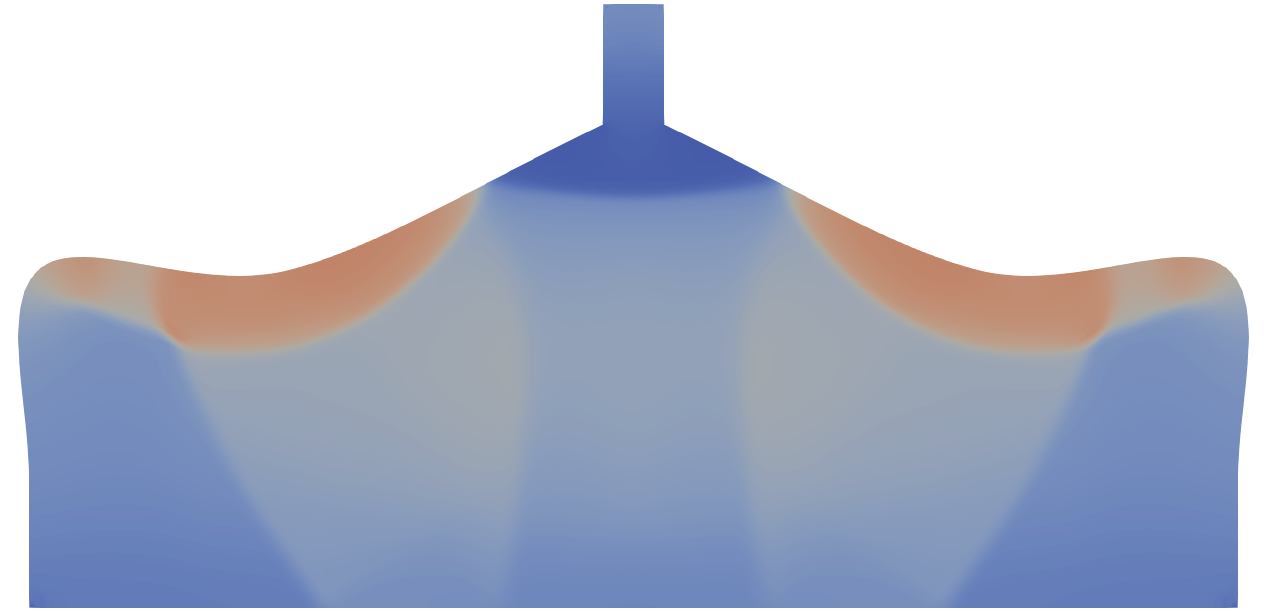
\includegraphics[width=0.96\textwidth]{pressure_field_case_6_type_2_08_10.png}
        \subcaption{}
    \end{subfigure}
    \captionsetup{font=scriptsize}
    \caption{
    Pressure contours at 4 time points (a:$\frac{1}{10}T$,b:$\frac{4}{10}T$,c:$\frac{6}{10}T$,d:$\frac{8}{10}T$) during the ``upward push half-cycle'' for the type 2 chamber under Case 6.
    Smoother upper part better alleviates ejection collision and resulting downward flow (a)(b);
``downward-curving'' further suppresses collision with new flow (d); collisions are more dispersed.
    }
    \label{fig:pressure_field_case_6_type_2}
\end{figure}

Compared to 1-control-point, max pressure is reached during ejection flow (Figure \ref{fig:pressure_field_case_6_type_2}a), pressure map is smoother.
Thus, it is better at suppressing bounce back; max pressure is better than 1-control-point.
Classification of bounce backs: 1. Ejection bounce flow still meets upward flow, but smoother upper wall makes ejection bounce and wave divergence milder (Figure \ref{fig:pressure_field_case_6_type_2}a);
2. Lower corner bounces are nearly horizontal (Figure \ref{fig:pressure_field_case_6_type_2}a,b,c), avoiding direct collision with downward bounce flow;
3. Collision between new flow, downward flow, and corner flows happens in stages and dispersed locations, not concentrated as in trapezoid.

\begin{figure}[htbp]
    %\centering
    \begin{subfigure}[b]{0.44\textwidth}
        \centering
        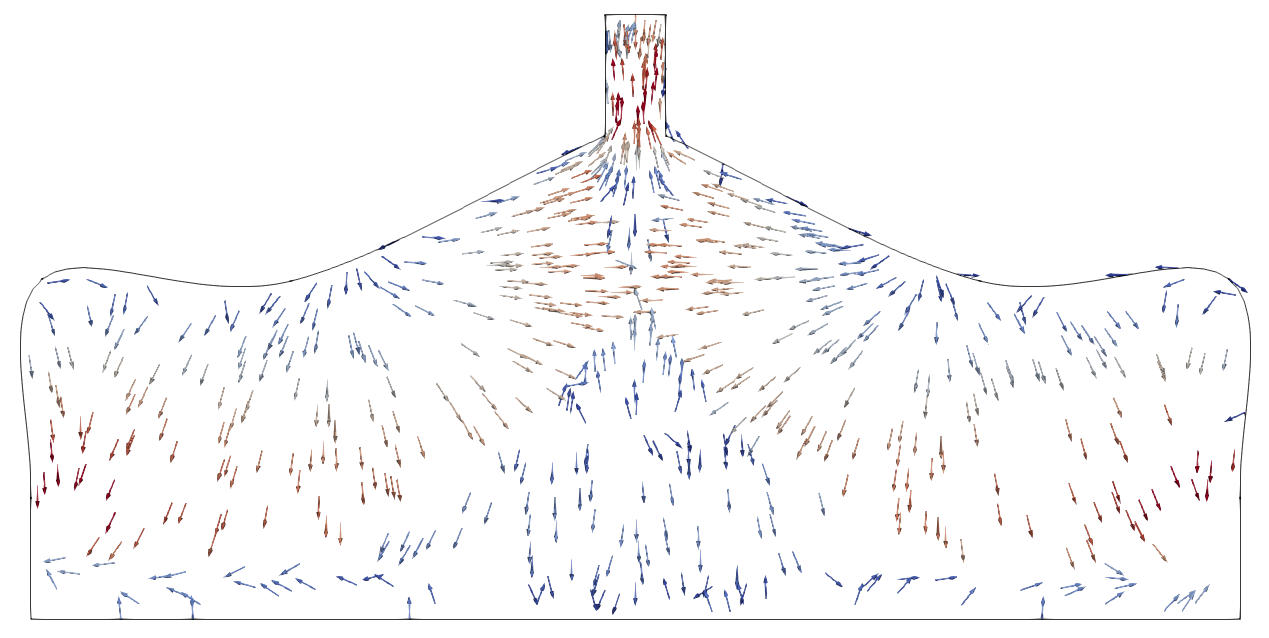
\includegraphics[width=0.96\textwidth]{velocity_field_case_6_type_2_01_10.png}
        \subcaption{}
    \end{subfigure}
    \begin{subfigure}[b]{0.44\textwidth}
        \centering
        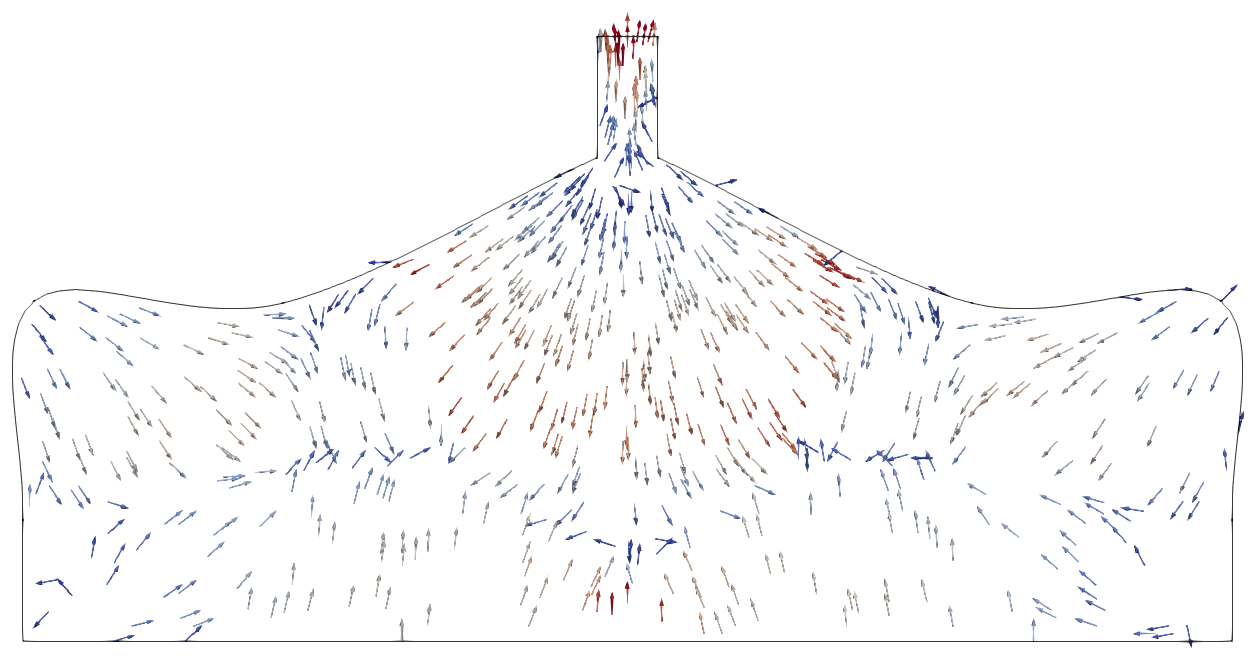
\includegraphics[width=0.96\textwidth]{velocity_field_case_6_type_2_04_10.png}
        \subcaption{}
    \end{subfigure}
    \begin{subfigure}[b]{0.10\textwidth}
        \centering
        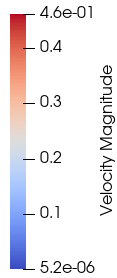
\includegraphics[width=0.96\textwidth]{velocity_field_case_6_type_2_axis.png}
        \vspace{1.0pt}
    \end{subfigure}
    \\
    \begin{subfigure}[b]{0.44\textwidth}
        \centering
        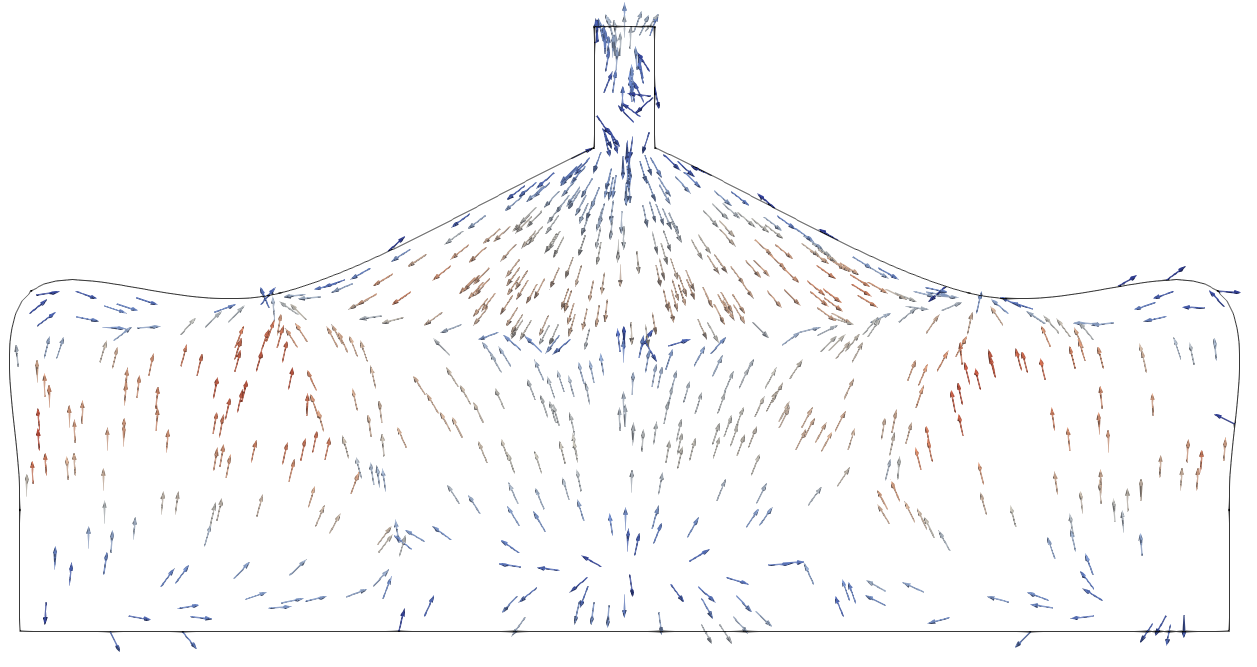
\includegraphics[width=0.96\textwidth]{velocity_field_case_6_type_2_06_10.png}
        \subcaption{}
    \end{subfigure}
    \begin{subfigure}[b]{0.44\textwidth}
        \centering
        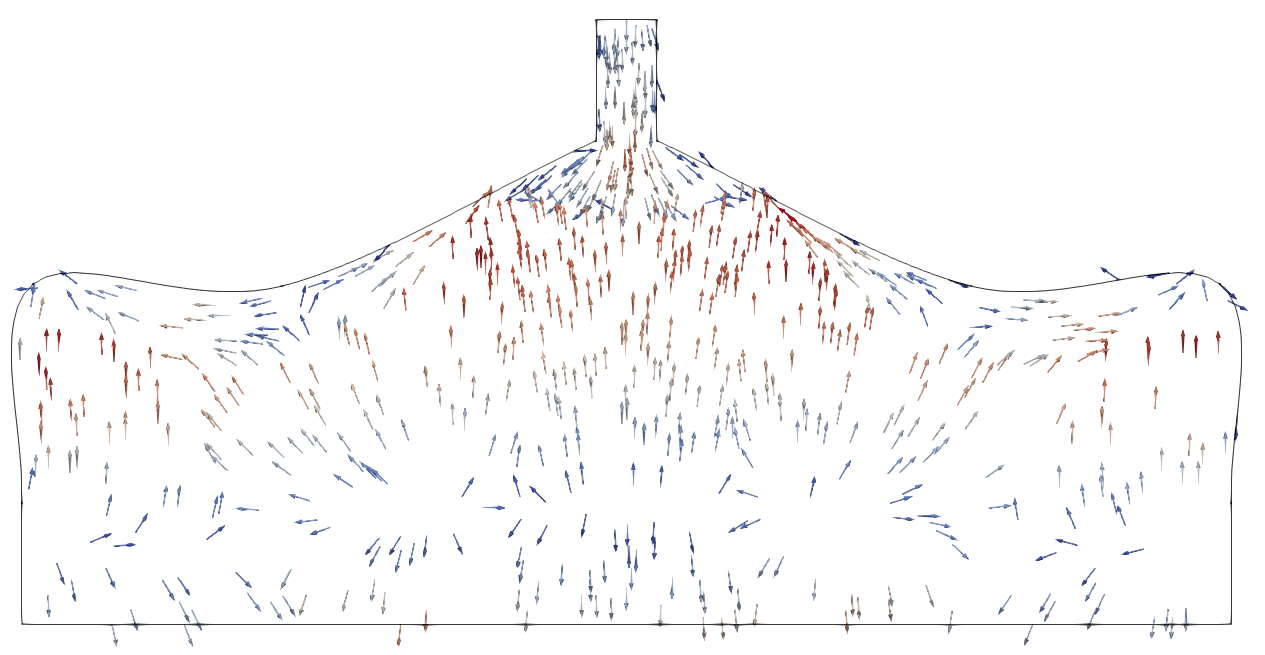
\includegraphics[width=0.96\textwidth]{velocity_field_case_6_type_2_08_10.png}
        \subcaption{}
    \end{subfigure}
    \captionsetup{font=scriptsize}
    \caption{
    Velocity vector diagrams at 4 time points (a:$\frac{1}{10}T$,b:$\frac{4}{10}T$,c:$\frac{6}{10}T$,d:$\frac{8}{10}T$) during the ``upward push half-cycle'' for the type 2 shape chamber under Case 6.
    Confirms multiple bounces, matching pressure contours.
    }
    \label{fig:velocity_field_case_6_type_2}
\end{figure}

Fluid morphology in Case 6 is complex and hard to describe simply.
Detailed discussion on this might deviate from optimization intent but is worth deep study.

Summary: Case 6 fluid has complex internal collisions and high intensity causing large pressure;
fluid even ``bounces'', inducing further collisions. This reminds researchers that simply increasing frequency doesn't necessarily improve outlet velocity.
RL-provided shapes (1 or 2 control points) specifically weaken these internal collisions. The two shapes optimize slightly differently.

This demonstrates the RL algorithm's ability to optimize for specific cases.
This paper found that in double amplitude/frequency cases, RL-given shapes and mechanisms differ from Case 0;
in low amplitude/frequency, ``inverted T'' dominates. Only Case 0 and Case 2 (height change) yielded ``S-shaped'', suggesting ``S-shape'' relates to geometry.
Recap of 9 physical parameters: 1. Synthetic jet internal flow is complex; Case 4/6 show that increasing amplitude/frequency won't necessarily yield better velocity;
2. Case 0 ``inverted T'' and ``S-shaped'' are reasonable but limited to lower frequency/amplitude; ``S-shaped'' may depend on geometry.

\subsection{Results and Analysis of Dynamic Mode Decomposition of Optimization Schemes}\indent

Although qualitative analysis of these optimized shapes has been conducted based on specific flow field pressure contours and velocity vector maps,
this paper still aims to further explore the flow characteristics and optimization mechanisms of these shapes under different physical parameters.
To further explore flow characteristics and optimization mechanisms, DMD is performed on velocity data of different shapes and parameters.
Specifically, Case 0, 4, 6 are analyzed.

Since SVD often yields complex eigenvalues, transformation matrix A contains complex numbers.
In 2D velocity, modal results for each direction have real/imaginary parts (4 components per moment).
Since eigenvalues sometimes only have real parts and real parts are used in cylinder flow DMD, real parts of modes corresponding to 2D velocity are analyzed.
Given flow complexity in vectors, analyzing just horizontal or vertical modes is insufficient; the magnitude (norm) of the two velocity modes is analyzed.
The dominant mode with the largest norm is analyzed.

Overall, first-order mode extrema appear in the intense outlet channel, consistent with synthetic jet principles;
Case 0 modes are smoother than Case 4 (double amplitude) or Case 6 (double frequency), where motion is more intense.

First, illustraing the analysis of Case 0 modes (Figure \ref{fig:dynamic_mode_decomposition_case_0_references}).

\begin{figure}[htbp]
    \centering
    \begin{subfigure}[b]{0.25\textwidth}
        \centering
        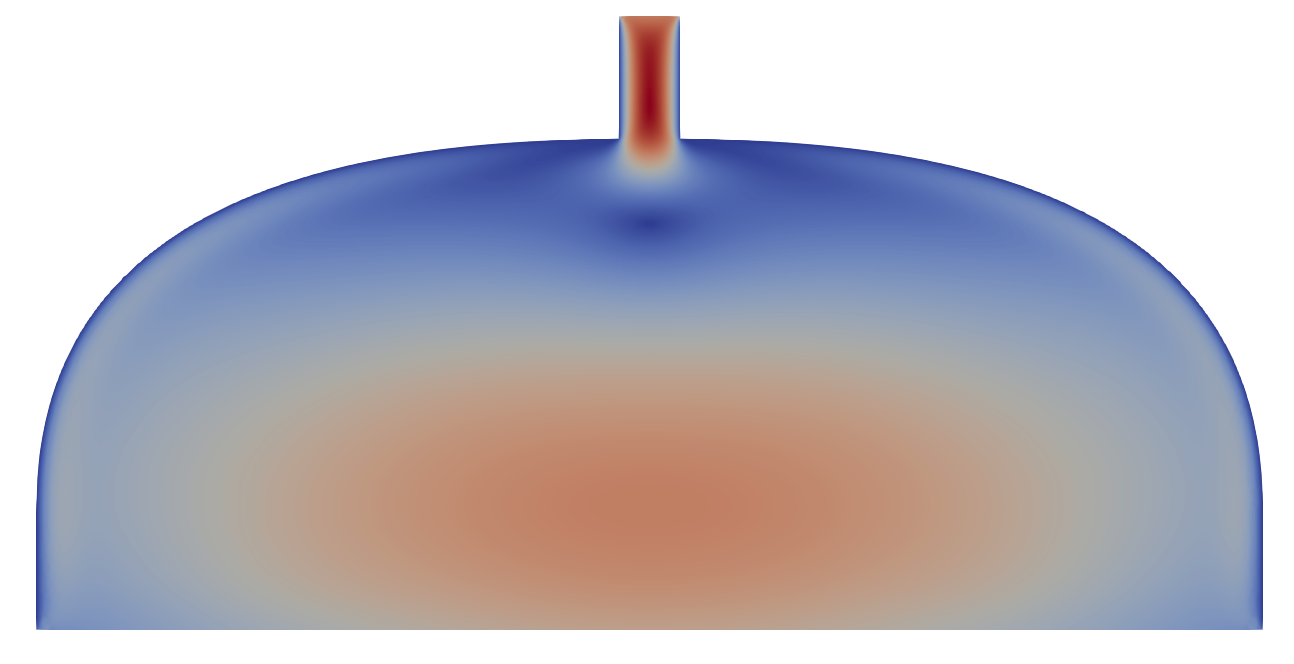
\includegraphics[width=0.96\textwidth]{dynamic_mode_decomposition_case_0_arched.png}
        \subcaption{}
    \end{subfigure}
    \begin{subfigure}[b]{0.06\textwidth}
        \centering
        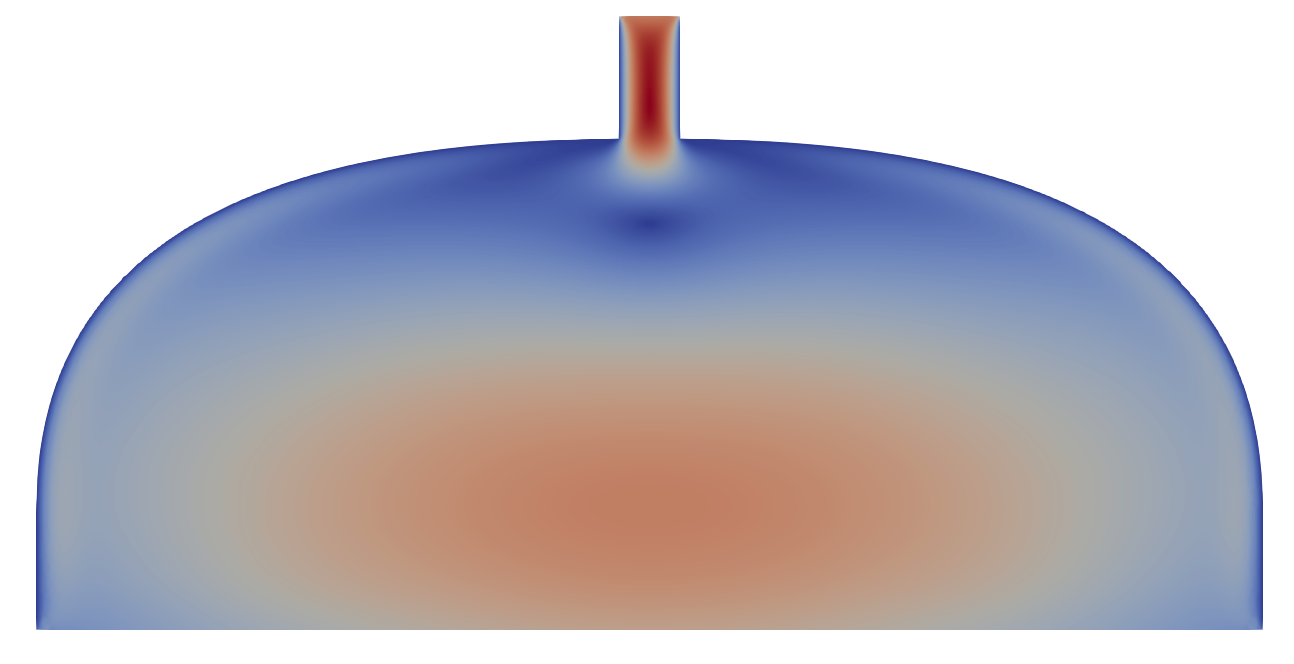
\includegraphics[width=0.96\textwidth]{dynamic_mode_decomposition_case_0_arched.png}
        \vspace{1.0pt}
    \end{subfigure}
    \begin{subfigure}[b]{0.25\textwidth}
        \centering
        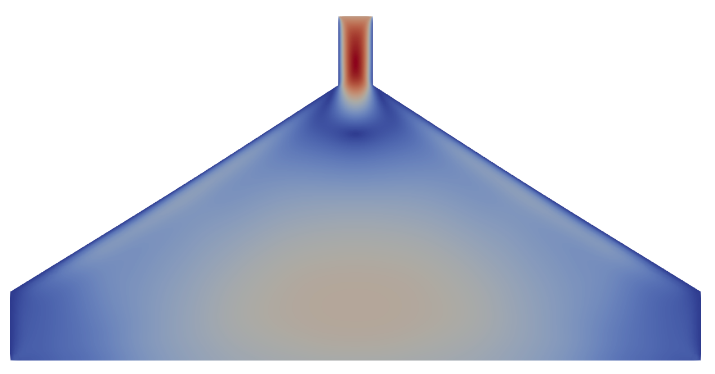
\includegraphics[width=0.96\textwidth]{dynamic_mode_decomposition_case_0_trapezoidal.png}
        \subcaption{}
    \end{subfigure}
    \begin{subfigure}[b]{0.06\textwidth}
        \centering
        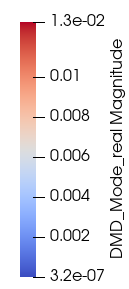
\includegraphics[width=0.96\textwidth]{dynamic_mode_decomposition_case_0_trapezoidal_axis.png}
        \vspace{1.0pt}
    \end{subfigure}
    \begin{subfigure}[b]{0.25\textwidth}
        \centering
        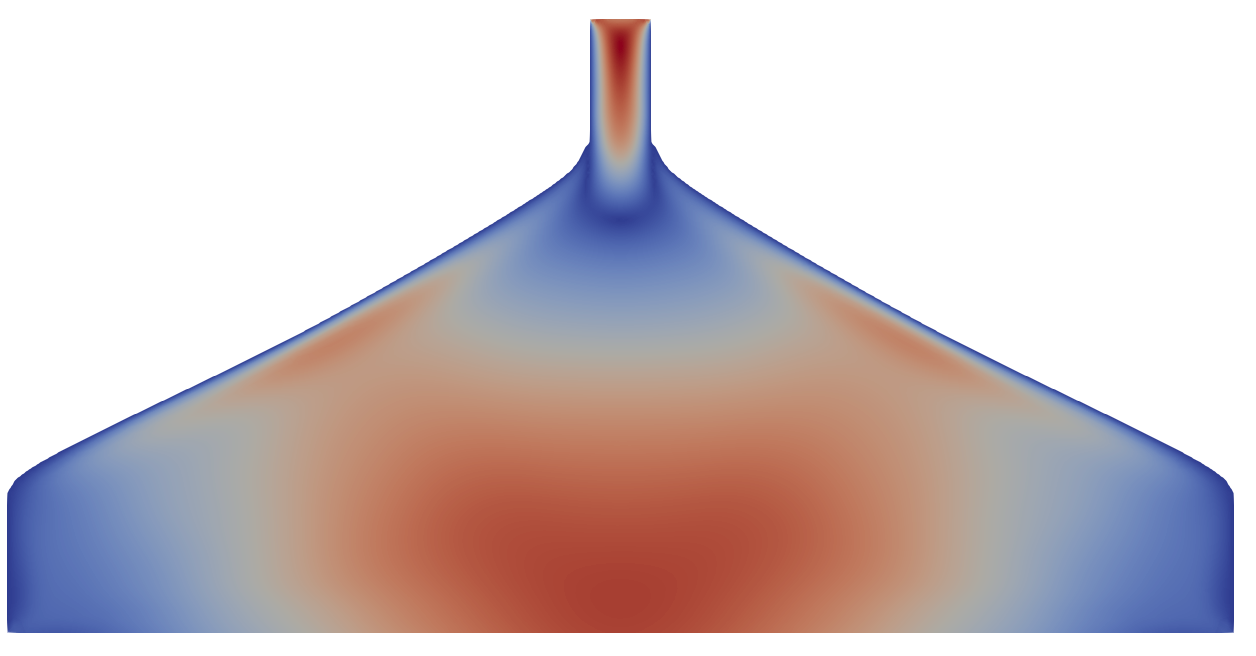
\includegraphics[width=0.96\textwidth]{dynamic_mode_decomposition_case_0_inverted_v.png}
        \subcaption{}
    \end{subfigure}
    \begin{subfigure}[b]{0.06\textwidth}
        \centering
        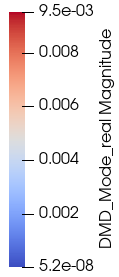
\includegraphics[width=0.96\textwidth]{dynamic_mode_decomposition_case_0_inverted_v_axis.png}
        \vspace{1.0pt}
    \end{subfigure}
    \captionsetup{font=scriptsize}
    \caption{
    DMD results for (a) arched, (b) trapezoidal, (c) ``inverted V''.
    Modes are smooth; trapezoid is larger (less collision, higher velocity);
    ``inverted V'' is lower, smooth transition may have hidden meaning.
    The modes within the three chamber shapes are relatively flat.
    The mode in the trapezoidal chamber is slightly larger; this may be related to the fact that the trapezoidal chamber shape weakens flow collisions during the ejection phase and increases the outlet velocity amplitude.
    The modal values for the ``inverted V-shape'' decrease significantly compared to the trapezoid; its smooth transition may hold some significance that was not reflected in the previous analysis. 
    }
    \label{fig:dynamic_mode_decomposition_case_0_references}
\end{figure}

Considering detailed DMD results, arched, trapezoidal, and ``inverted V'' modes are relatively smooth, with large values only at the outlet.
Trapezoidal modes are slightly larger than arched. Previous analysis suggested trapezoidal/``inverted V'' reduces ejection collisions to gain higher outlet velocity.
This modal result may support that.

On the other hand, ``Inverted V'' transitions at ends don't significantly affect pressure integral or max pressure; actual performance is similar to trapezoid.
However, ``inverted V'' mode distribution is more uniform and magnitude is slightly smaller (Figure \ref{fig:dynamic_mode_decomposition_case_0_references}).
This suggests smooth transitions have significance not captured in previous analysis.

\begin{figure}[htbp]
    \centering
    \begin{subfigure}[b]{0.40\textwidth}
        \centering
        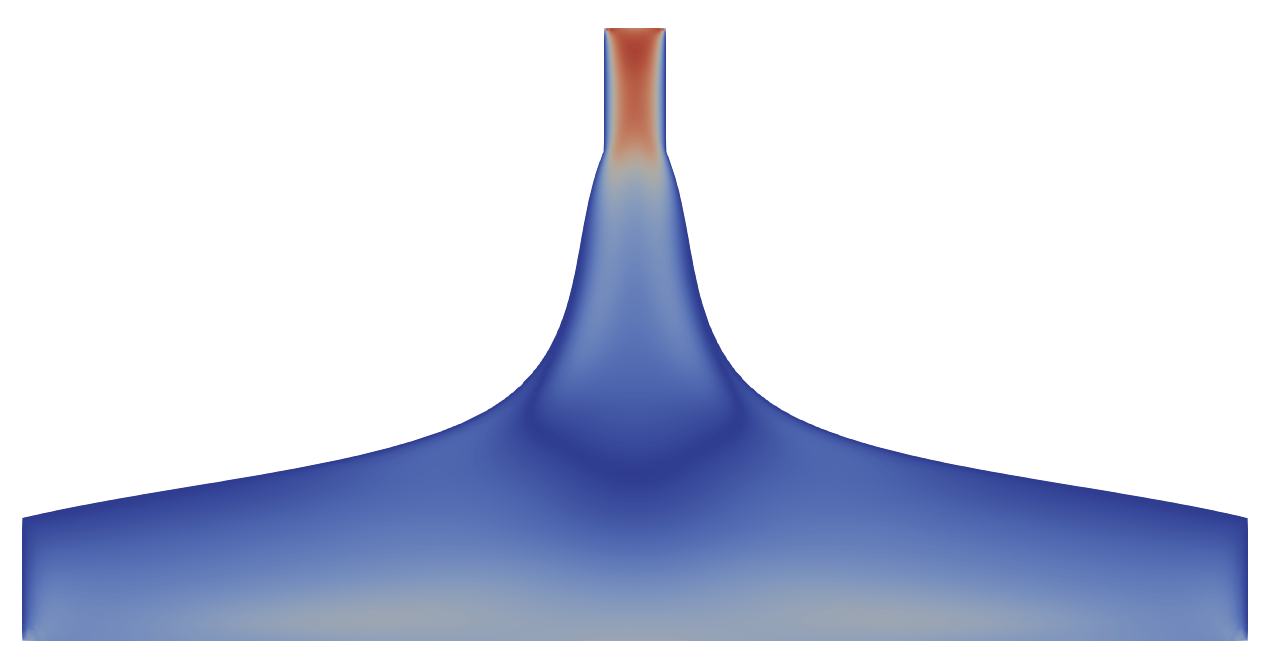
\includegraphics[width=0.96\textwidth]{dynamic_mode_decomposition_case_0_inverted_t.png}
        \subcaption{}
    \end{subfigure}
    \begin{subfigure}[b]{0.08\textwidth}
        \centering
        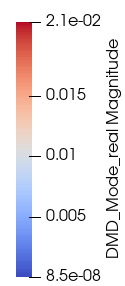
\includegraphics[width=0.96\textwidth]{dynamic_mode_decomposition_case_0_inverted_t_axis.png}
        \vspace{1.0pt}
    \end{subfigure}
    \begin{subfigure}[b]{0.40\textwidth}
        \centering
        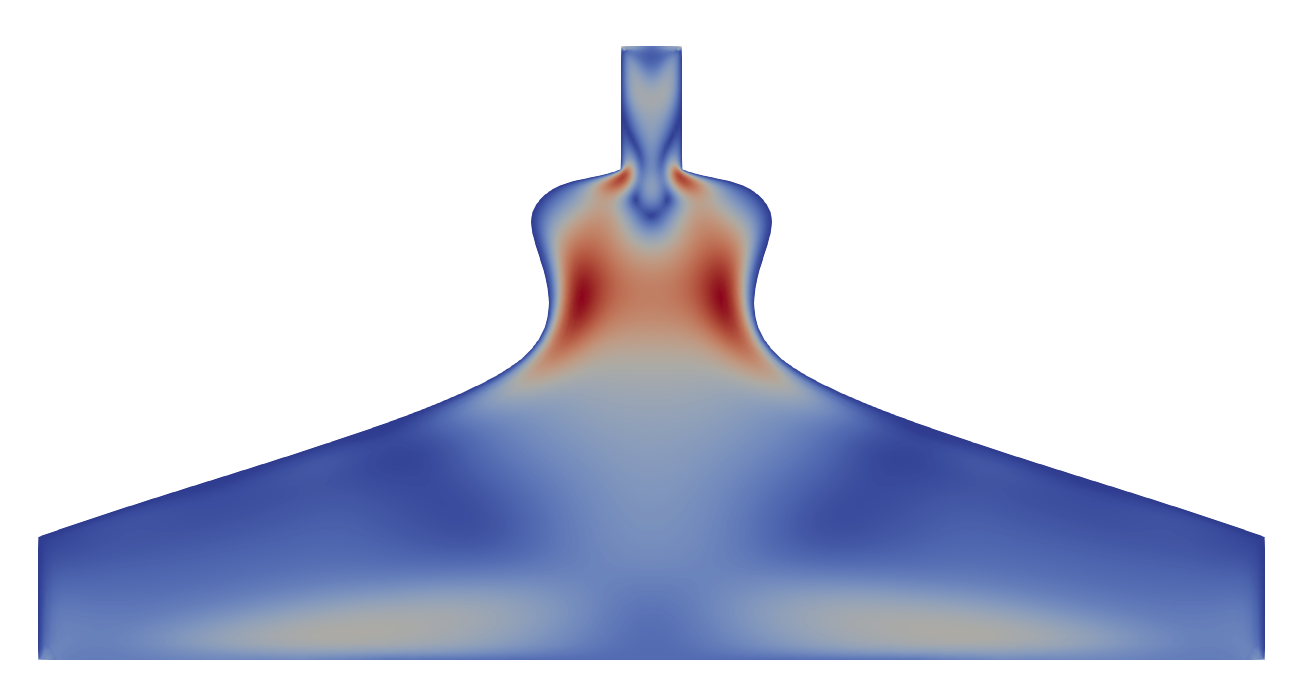
\includegraphics[width=0.96\textwidth]{dynamic_mode_decomposition_case_0_inverted_t_derivative.png}
        \subcaption{}
    \end{subfigure}
    \begin{subfigure}[b]{0.08\textwidth}
        \centering
        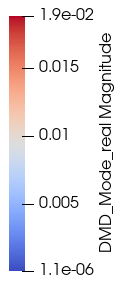
\includegraphics[width=0.96\textwidth]{dynamic_mode_decomposition_case_0_inverted_t_derivative_axis.png}
        \vspace{1.0pt}
    \end{subfigure}
    \captionsetup{font=scriptsize}
    \caption{
    Case 0 DMD results for (a) ``inverted T'' and (b) derivative.
    ``Inverted T'' values are at outlet; derivative's max decreases and moves into chamber with more uniform distribution.
    The ``Inverted T'' and its derivative may lower the tensity of fluid motion to a certain extent.
    }
    \label{fig:dynamic_mode_decomposition_case_0_inverted_t}
\end{figure}

``Inverted T'' and derivative modes are shown in Figure \ref{fig:dynamic_mode_decomposition_case_0_inverted_t}.
``Inverted T'' differs significantly from trapezoid; large values are almost all at the outlet, while the chamber is blue (small).
This may relate to ``inverted T'' features: collisions in lower chamber where velocity is low; fewer ejection collisions.
In the derivative shape, max mode value shifts from outlet into the chamber.
These results suggest ``inverted T'' and derivatives reduce flow intensity in the chamber to some extent.

``S-shaped'' and derivative modes (Figure \ref{fig:dynamic_mode_decomposition_case_0_s}) are more uniform, not limited to outlet.
Max positions vary, possibly due to ``curved pockets''. Previous analysis called them ``fluid buffer zones'' with low velocity.
Low modal values in pockets support this.

\begin{figure}[htbp]
    \centering
    \begin{subfigure}[b]{0.40\textwidth}
        \centering
        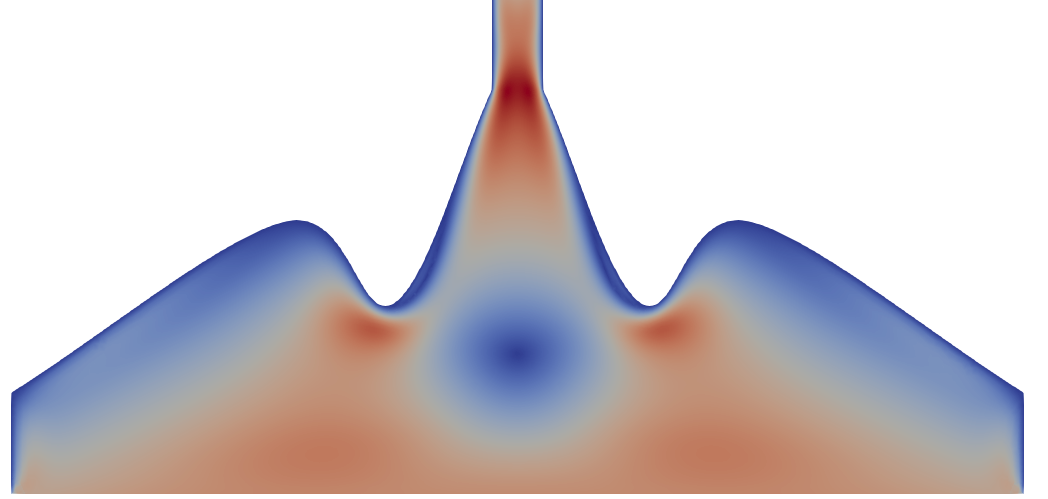
\includegraphics[width=0.96\textwidth]{dynamic_mode_decomposition_case_0_s.png}
        \subcaption{}
    \end{subfigure}
    \begin{subfigure}[b]{0.08\textwidth}
        \centering
        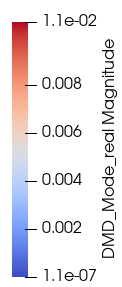
\includegraphics[width=0.96\textwidth]{dynamic_mode_decomposition_case_0_s_axis.png}
        \vspace{1.0pt}
    \end{subfigure}
    \begin{subfigure}[b]{0.40\textwidth}
        \centering
        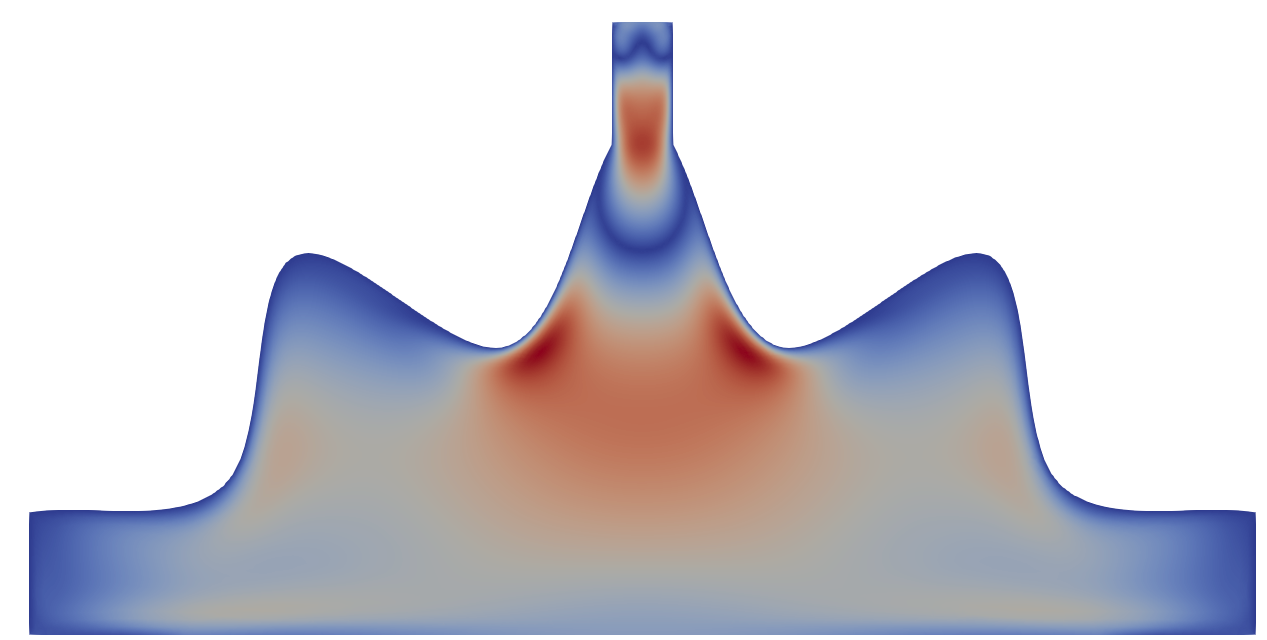
\includegraphics[width=0.96\textwidth]{dynamic_mode_decomposition_case_0_s_derivative.png}
        \subcaption{}
    \end{subfigure}
    \begin{subfigure}[b]{0.08\textwidth}
        \centering
        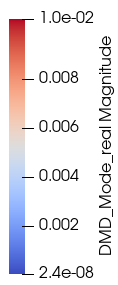
\includegraphics[width=0.96\textwidth]{dynamic_mode_decomposition_case_0_s_derivative_axis.png}
        \vspace{1.0pt}
    \end{subfigure}
    \captionsetup{font=scriptsize}
    \caption{
    Case 0 DMD results for (a) ``S'' and (b) derivative.
    More uniform distribution.
    Low pocket values match ``buffer zone'' view.
    Max value shifts downward.
    The modal distribution under the ``S-shape'' and its derivative shapes is more uniform.
    The modal values within the ``arc-shaped pocket'' are smaller, which may correspond to the previous viewpoint that the fluid within the ``arc-shaped'' pocket acts as a ``fluid buffer zone."
    From the modal results, the presence of the ``arc-shaped pocket'' also seems to cause a downward shift in the position where the maximum modal values occur.
    The ``S-shape'' and its derivative shapes may, to some extent, reduce the intensity of fluid motion within the chamber.
    }
    \label{fig:dynamic_mode_decomposition_case_0_s}
\end{figure}

``Inverted T'' results in smaller chamber modes; derivative and ``S-shaped'' make modes more uniform and shift max positions downward.
Speculation: they reduce flow intensity in the chamber.

Modes there chamber shapes under Case 4 modes are shown in Figure \ref{fig:dynamic_mode_decomposition_case_4}.
Case 4 only doubled amplitude.

\begin{figure}[htbp]
    \centering
    \begin{subfigure}[b]{0.25\textwidth}
        \centering
        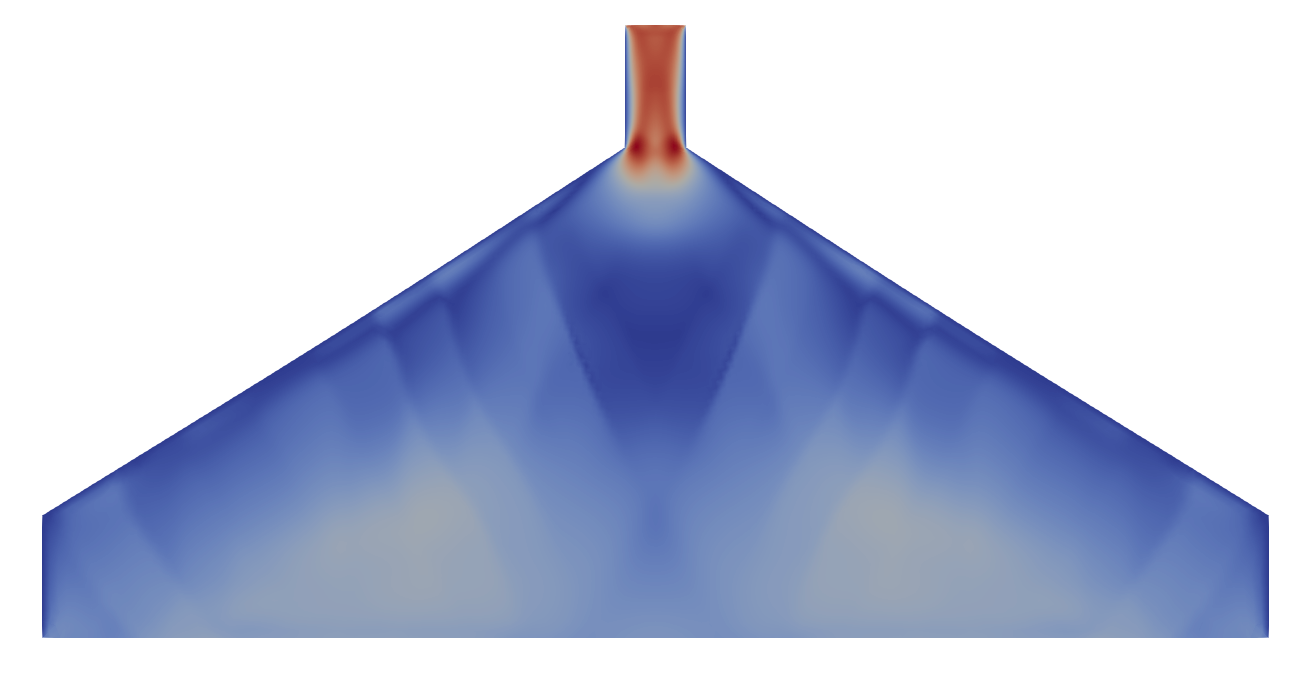
\includegraphics[width=0.96\textwidth]{dynamic_mode_decomposition_case_4_trapezoidal.png}
        \subcaption{}
    \end{subfigure}
    \begin{subfigure}[b]{0.06\textwidth}
        \centering
        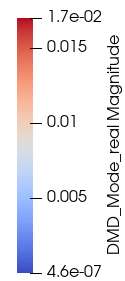
\includegraphics[width=0.96\textwidth]{dynamic_mode_decomposition_case_4_trapezoidal_axis.png}
        \vspace{1.0pt}
    \end{subfigure}
    \begin{subfigure}[b]{0.25\textwidth}
        \centering
        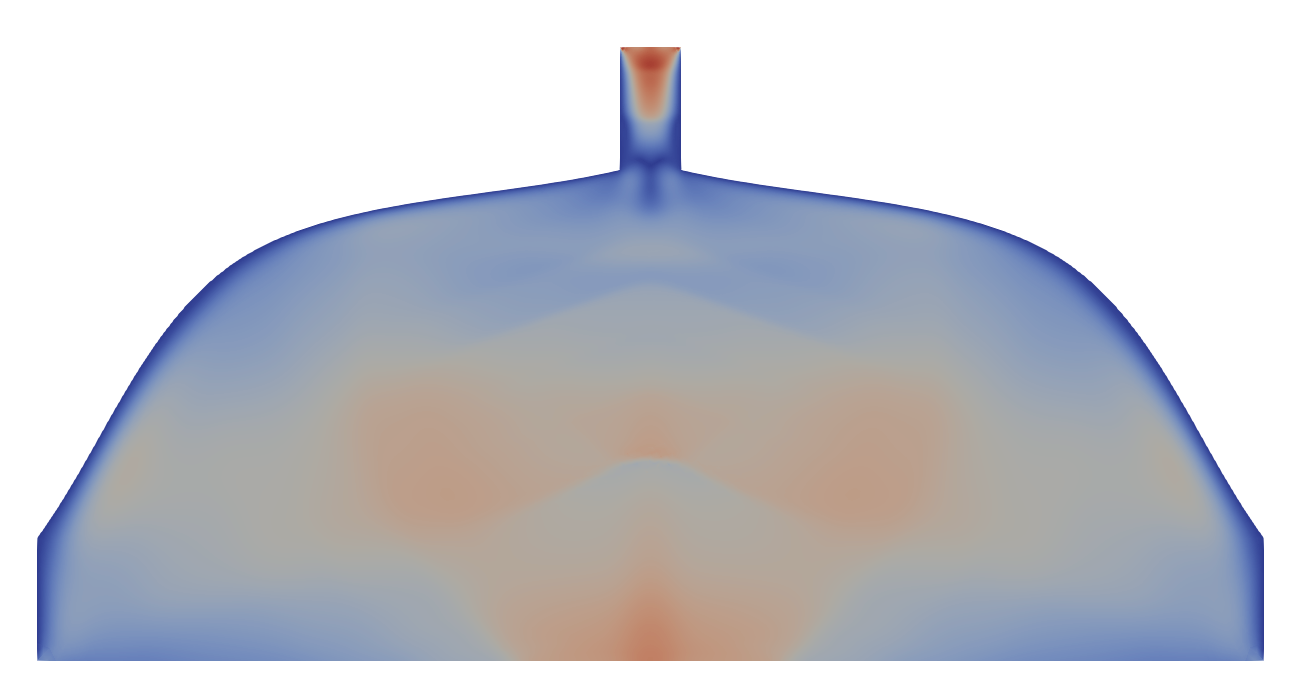
\includegraphics[width=0.96\textwidth]{dynamic_mode_decomposition_case_4_arched_1.png}
        \subcaption{}
    \end{subfigure}
    \begin{subfigure}[b]{0.06\textwidth}
        \centering
        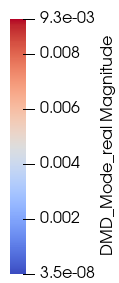
\includegraphics[width=0.96\textwidth]{dynamic_mode_decomposition_case_4_arched_1_axis.png}
        \vspace{1.0pt}
    \end{subfigure}
    \begin{subfigure}[b]{0.25\textwidth}
        \centering
        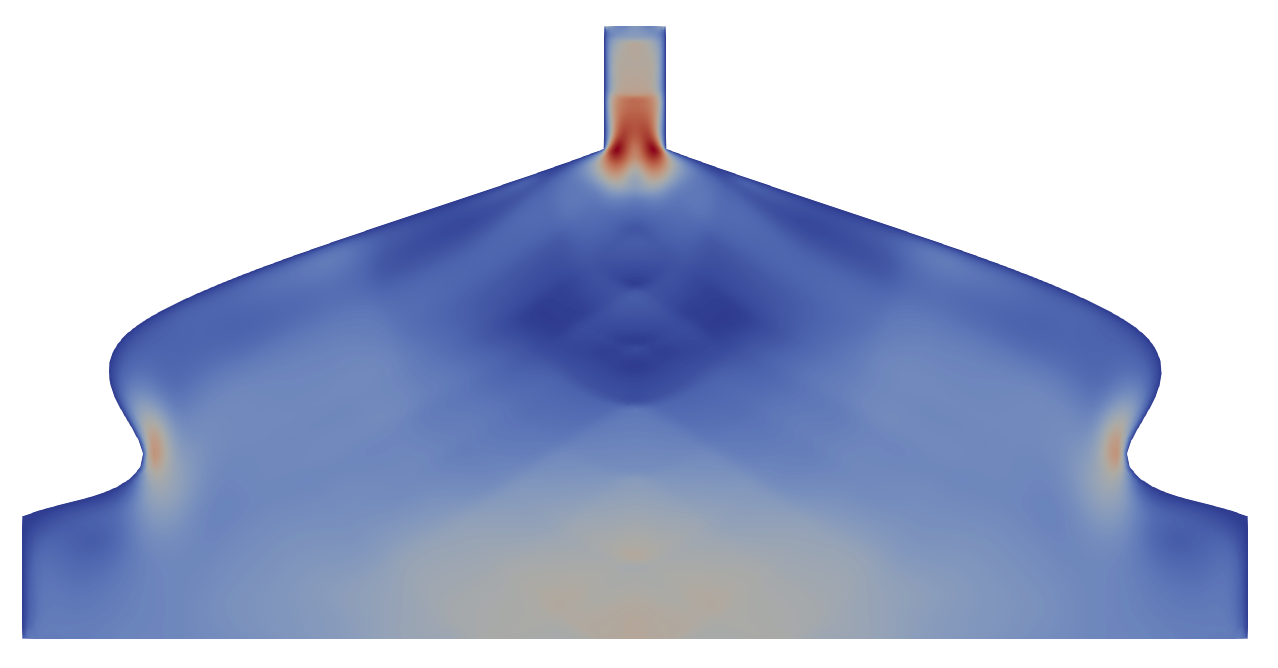
\includegraphics[width=0.96\textwidth]{dynamic_mode_decomposition_case_4_arched_2.png}
        \subcaption{}
    \end{subfigure}
    \begin{subfigure}[b]{0.06\textwidth}
        \centering
        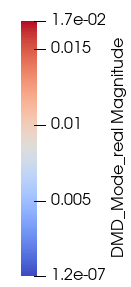
\includegraphics[width=0.96\textwidth]{dynamic_mode_decomposition_case_4_arched_2_axis.png}
        \vspace{1.0pt}
    \end{subfigure}
    \captionsetup{font=scriptsize}
    \caption{
    Case 4 DMD results for (a) trapezoidal and (b) arched shape using 1 and (c) 2 control points.
    Modes show ``textures'', likely related to intense flow and pressure wave divergence.
    Optimization changes textures from longitudinal to transverse, likely related to alleviating divergence effects on walls.
    1-control-point is more uniform than 2. DMD gives information not seen in direct flow observation. 
    }
    \label{fig:dynamic_mode_decomposition_case_4}
\end{figure}

Previous analysis saw more intense flow in Case 4, especially pressure wave divergence during ejection.
Case 4 modes for all three shapes contain textures, reflecting complex flow features.
In trapezoidal, textures are longitudinal; in optimized shapes, they are transverse.
This change probably relates to alleviating ejection pressure wave divergence.
Analysis considered 1 vs 2 control point shapes similar, but modal results differ significantly (Figure \ref{fig:dynamic_mode_decomposition_case_4}b,c).
DMD shows previous analysis missed some factors.

Modes there chamber shapes under Case 6 modes are shown in Figure \ref{fig:dynamic_mode_decomposition_case_6}.
Case 6 only doubled frequency.

\begin{figure}[htbp]
    \centering
    \begin{subfigure}[b]{0.25\textwidth}
        \centering
        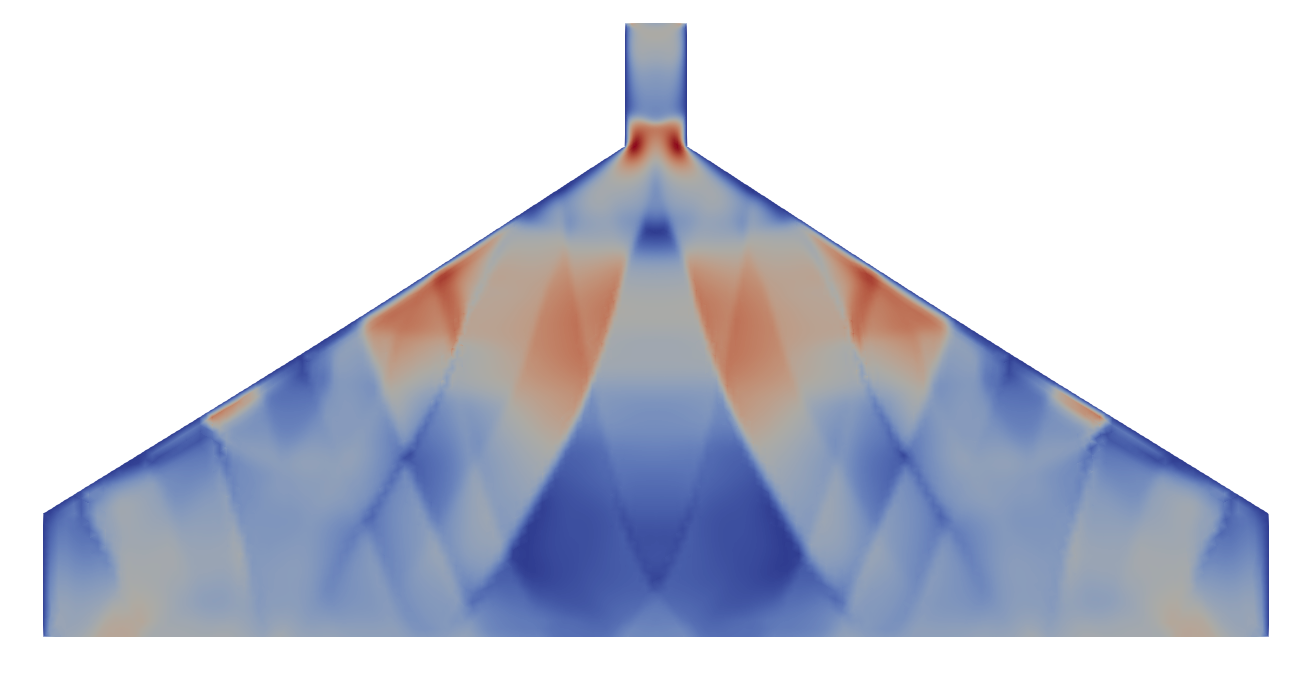
\includegraphics[width=0.96\textwidth]{dynamic_mode_decomposition_case_6_trapezoidal.png}
        \subcaption{}
    \end{subfigure}
    \begin{subfigure}[b]{0.06\textwidth}
        \centering
        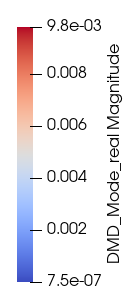
\includegraphics[width=0.96\textwidth]{dynamic_mode_decomposition_case_6_trapezoidal_axis.png}
        \vspace{1.0pt}
    \end{subfigure}
    \begin{subfigure}[b]{0.25\textwidth}
        \centering
        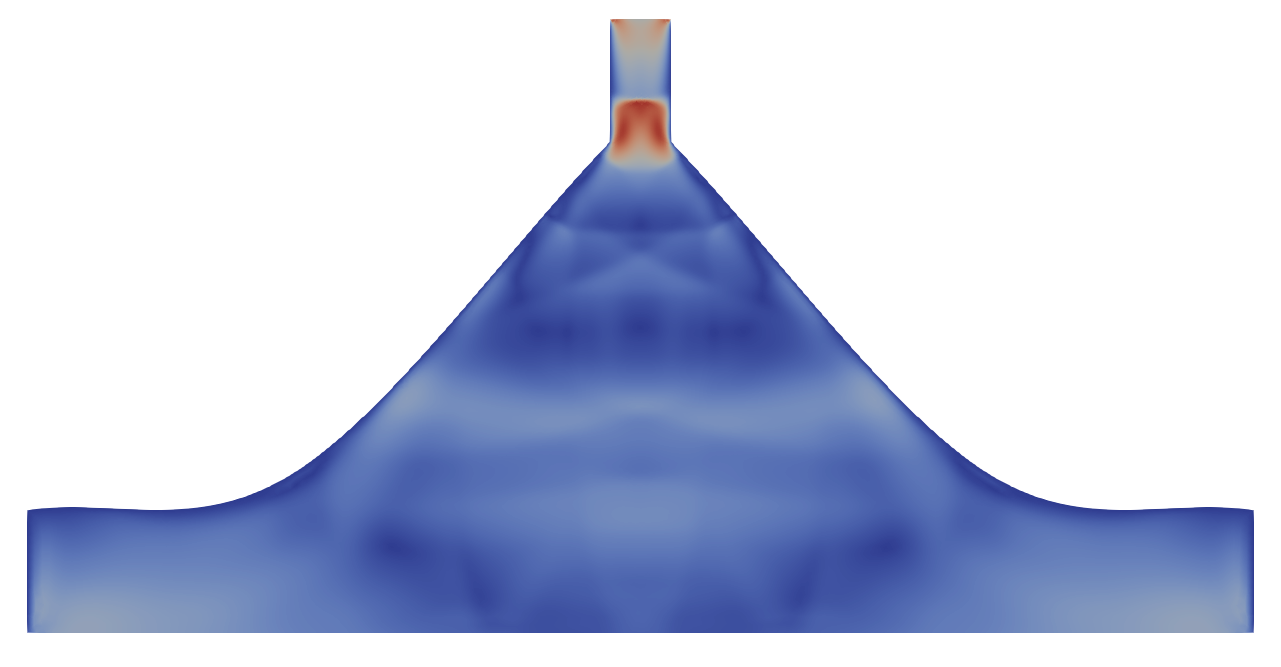
\includegraphics[width=0.96\textwidth]{dynamic_mode_decomposition_case_6_type_1.png}
        \subcaption{}
    \end{subfigure}
    \begin{subfigure}[b]{0.06\textwidth}
        \centering
        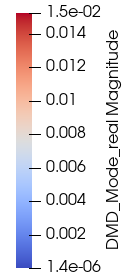
\includegraphics[width=0.96\textwidth]{dynamic_mode_decomposition_case_6_type_1_axis.png}
        \vspace{1.0pt}
    \end{subfigure}
    \begin{subfigure}[b]{0.25\textwidth}
        \centering
        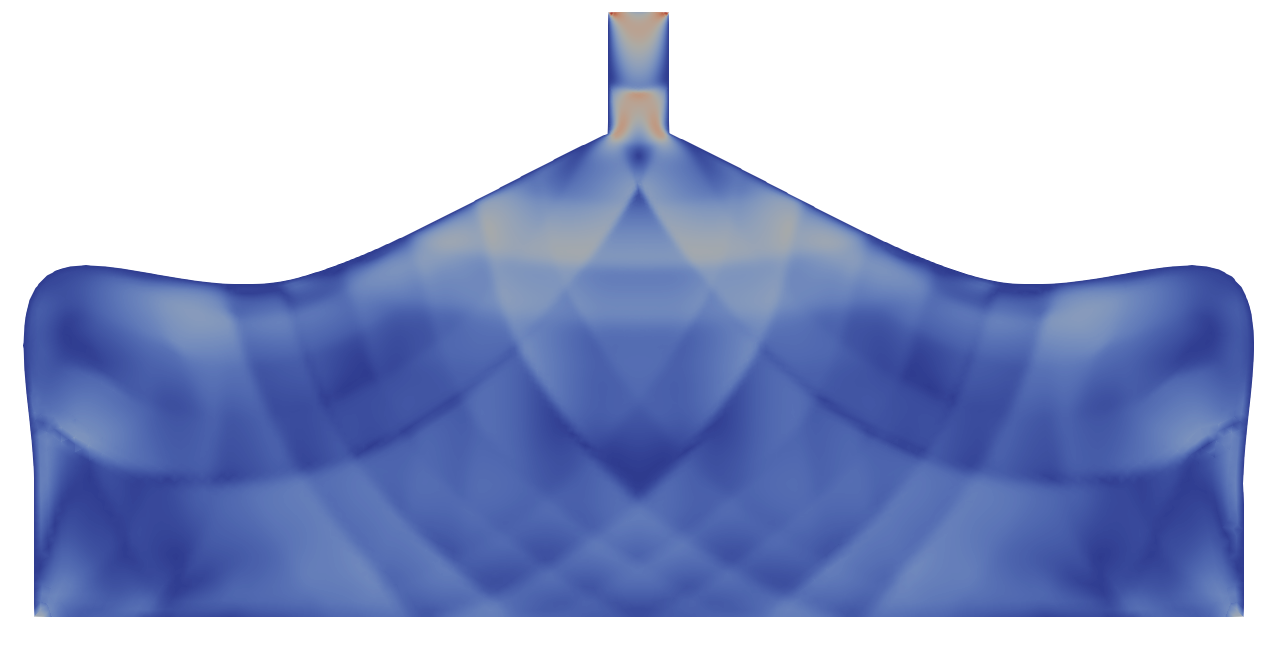
\includegraphics[width=0.96\textwidth]{dynamic_mode_decomposition_case_6_type_2.png}
        \subcaption{}
    \end{subfigure}
    \begin{subfigure}[b]{0.06\textwidth}
        \centering
        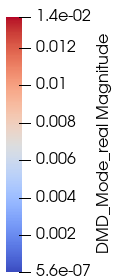
\includegraphics[width=0.96\textwidth]{dynamic_mode_decomposition_case_6_type_2_axis.png}
        \vspace{1.0pt}
    \end{subfigure}
    \captionsetup{font=scriptsize}
    \caption{
    Case 6 DMD results for (a) trapezoidal, (b) type 1 using 1-control-point, (c) type 2 using 2-control-point.
    Complex textures match bounce back. Optimized chamber values are small.
    Max pressure at outlet for 1-control-point matches analysis of its upper chamber smoothness.
    The modal results of Case 6 exhibit more complex textures than those in Case 4, perhaps corresponding to the previously observed complex collision and rebound phenomena.
    Compared to the trapezoid, the modal values for both optimized shapes within the chamber are very small.
    Previous analysis suggested that both optimized shapes mitigate the collision between the downward flow caused by ejection-phase rebound and the incoming flow of the new cycle.
    However, due to the difference in the smoothness of the upper chamber between the two, the maximum wall pressure of the optimized shape with one control point still reaches a relatively large value at the outlet during the ejection phase.
    The modal results seem to support this analysis.
    }
    \label{fig:dynamic_mode_decomposition_case_6}
\end{figure}

Previous analysis saw more intense flow and bounce back in Case 6.
Case 6 modes show more complex textures than Case 4, likely due to bounce back.
Analysis suggested optimized shapes alleviate collision between bounce flow and new incoming flow;
chamber modal values are very small (Figure \ref{fig:dynamic_mode_decomposition_case_6}b,c), supporting this.
Previously, 2-control-point was seen as smoother and better at alleviating ejection bounce (Figure \ref{fig:dynamic_mode_decomposition_case_6}c).
1-control-point max is at outlet, while 2-control-point is overall smaller, supporting this.

Summary: DMD results generally correspond to flow information analysis and provide additional insights.

\section*{Conclusions}
\addtocounter{section}{1}
\setcounter{subsection}{0}
\addcontentsline{toc}{section}{\protect\numberline{}Conclusions}\indent

Synthetic jets possess unique zero-mass characteristics; they do not require additional fluid injection during operation, offering distinct advantages over traditional flow control methods.
However, the fluid motion within synthetic jet devices is often highly intense, and the chamber walls are frequently subjected to significant pressure, which places high demands on the structural strength of the device.
Unlike traditional flow device geometry optimization that relies on experience, this thesis employs machine learning methods combined with Computational Fluid Dynamics (CFD).
Various reinforcement learning algorithms and different numbers of control points are used to perform chamber shape optimization for synthetic jet devices under multiple sets of physical parameters.
The goal is to reduce the pressure borne by the chamber walls while ensuring outlet velocity performance.
Specifically, the wall pressure integral, maximum wall pressure, and outlet velocity amplitude were taken as optimization targets.
Among these, the wall pressure integral is related to the curve length of the wall and serves as a secondary optimization target.
Traditionally, geometric shape optimization of flow devices is a difficult task.
Determining which parameters might influence the optimization target and establishing the extent of that influence relies heavily on experience.
This thesis limits the ``behavior'' of the reinforcement learning algorithm as little as possible.
To support this, a comprehensive program robustness setting was established to give the reinforcement learning algorithm room for exploration and trial-and-error.
This achieved chamber shape optimization independent of manual experience, yielding unexpected but high-performance optimized shapes.
The flow mechanisms of these optimized shapes were then analyzed based on CFD numerical simulations.
In the first set of physical parameters attempted, reinforcement learning produced various optimized shapes such as the ``Inverted T-shape'', ``S-shape'', and their derivatives, rather than the expected ``Inverted V-shape''.
An analysis was conducted on the rationality of the ``Inverted T-shape'' and S-shape'', and why the reinforcement learning algorithm preferred these two over the ``Inverted V-shape'', which had very similar performance and was more in line with expectations.
As more physical parameter conditions were tested, the researcher realized that the ``Inverted T-shape'' and ``S-shape'' might be more suitable for lower amplitudes and lower frequencies, and the ``S-shape'' might even have certain geometric dependencies.
At higher amplitudes and frequencies, the flow field patterns within the chamber changed significantly, and the reinforcement learning algorithm provided targeted optimization shapes different from the ``Inverted T-shape'' and ``S-shape'' for these patterns.
This thesis also analyzed the optimization mechanisms of these shapes.
These attempts revealed the complexity of the synthetic jet device itself.
In the design of synthetic jet devices, a comprehensive optimization result often cannot be achieved by changing a single parameter in isolation.
This, in turn, confirms the effectiveness, or rather the learning capability, of reinforcement learning algorithms.

\section*{Outlook}
\addtocounter{section}{1}
\setcounter{subsection}{0}
\addcontentsline{toc}{section}{\protect\numberline{}Outlook}\indent

From the perspective of synthetic jet device optimization, this thesis explored the flow mechanisms and corresponding chamber design optimization mechanisms under different physical parameters.
The distinct optimized shapes obtained through reinforcement learning algorithms and the flow mechanism analysis of these shapes can provide references and ideas for subsequent theoretical research or practical production and manufacturing.
Regarding the general patterns of applying reinforcement learning methods, this thesis demonstrates that reinforcement learning algorithms can process given problems according to ``their own'' ideas and provide excellent solutions beyond expectations for specific situations, confirming the effectiveness and creativity of reinforcement learning algorithms.
The creativity of reinforcement learning algorithms is likely to provide brand-new ideas for subsequent research.
Of course, this thesis also has many shortcomings and areas yet to be addressed.
1.Even considering all selected physical parameters, the parameters chosen in this thesis still have significant limitations.
The generalizability of the discussions made within this limited range remains to be verified.
Furthermore, this thesis presupposes that the chamber is left-right symmetrical; if the coupling of the synthetic jet device with other flows is considered, an asymmetrical chamber might exhibit better performance and bring more inspiration.
2.Due to limited computational power, this thesis did not fully explore the impact of the number of control points on the optimization scheme, especially noting that better-performing optimized shapes can sometimes be obtained with more control points.
3.Regarding the optimization mechanisms of the designs appearing in this thesis, only some qualitative analyses were performed; there is a lack of detailed analysis of the flow field characteristics at higher frequencies and higher amplitudes.
Additionally, there are some technical shortcomings in this thesis.
For instance, the specific hyperparameters of the reinforcement learning algorithms used were not modified;
the ``control points + connecting curves'' scheme used for chamber shape generation might not be the most appropriate (which may have affected optimization results);
reward calculation relied on manual tuning (perhaps inverted reinforcement learning could be introduced);
parallelism (computational demand) or imitation learning (preset ``behavioral tendencies'') were not used to improve model training under multiple control points;
and separate models were trained for different physical parameters rather than training a composite model.
These deficiencies remain to be further refined in future research.

\end{document}

